\documentclass[a4paper]{article}   	% use "amsart" instead of "article" for AMSLaTeX format
\usepackage{geometry}                		% See geometry.pdf to learn the layout options. There are lots.
\geometry{left=1.5cm,right=1.5cm,top=1.5cm,bottom=1.5cm}                   		
\usepackage{graphicx,subcaption}					
\usepackage{amssymb}
\usepackage{indentfirst}
\usepackage{amsmath}
\usepackage{amsthm}
\usepackage{bm}
\usepackage{lineno}
\usepackage{setspace}
\usepackage{booktabs,multirow}
\usepackage{authblk}

\RequirePackage[colorlinks,citecolor=blue,urlcolor=blue]{hyperref}

\newtheorem{theorem}{Theorem}
\newtheorem{lemma}[theorem]{Lemma}
\newtheorem{corollary}[theorem]{Corollary}
\newcommand{\E}{\mathrm{E}}
\newcommand{\D}{\mathcal{MD}}
\newcommand{\Var}{\mathrm{Var}}
\newcommand{\Cov}{\mathrm{Cov}}
\newcommand{\Corr}{\mathrm{Corr}}
\newcommand{\tr}{\mathrm{tr}}
\newcommand{\R}{\texttt{R}}
\newcommand{\asreml}{\texttt{ASReml-R}}
\newcommand{\brms}{\texttt{brms}}
\newcommand{\rstan}{\texttt{rstan}}
\newcommand{\elpd}{elpd\textsubscript{loo}}
\newcommand{\psis}{elpd\textsubscript{psis-loo}}
\newcommand{\ploo}{p\textsubscript{loo}}

\newcommand{\BigO}[1]{{\rm O}\left(#1\right)}
\newcommand{\eg}{e.g.\ }
\newcommand{\ie}{i.e.\ }
\newcommand{\iid}{\textrm{i.i.d.\ }}
\newcommand{\N}{\mathcal{N}}
\newcommand{\AR}{\mathrm{AR}1}
\newcommand{\Matern}{Mat\'ern }

\usepackage[url=false, isbn=false, eprint=false, backref=true, style= authoryear, backend=bibtex, maxcitenames=2, giveninits=true, maxbibnames=100]{biblatex}
\addbibresource{BayesOFE.bib}

\title{Bayesian Inference of Spatially Correlated Random Parameters for On-farm Experiment}
%\author{Jerome}
\author[1]{Zhanglong Cao}
\author[1]{Katia Stefanova}
\author[1,2]{Mark Gibberd}
\author[1,3]{Suman Rakshit}

\affil[1]{SAGI West, School of Molecular and Life Sciences, Curtin University, Perth, Australia}
\affil[2]{Centre for Crop and Disease Management, School of Molecular and Life Sciences, Curtin University, Perth, Australia}
\affil[3]{School of Electrical Engineering, Computing, and Mathematical Sciences, Curtin University, Perth, Australia}

\date{}							% Activate to display a given date or no date

\linenumbers
\doublespacing
% \onehalfspacing

\begin{document}
	
	\maketitle
	
	\begin{abstract}
		Accounting for spatial variability is crucial while estimating treatment effects in large on-farm trials. It allows to determine the optimal treatment for every part of a paddock, resulting in a management strategy that improves sustainability and profitability of the farm. We specify a model with spatially correlated random parameters to account for the spatial variability in large on-farm trials. A Bayesian framework has been adopted to estimate the posterior distribution of these parameters. By accounting for spatial variability, this framework  allows the estimation of spatially-varying treatment effects in large on-farm trials. Several approaches have been proposed in the past for assessing spatial variability. However, these approaches lack an adequate discussion of the potential problem of model misspecification. Often the Gaussian distribution is assumed for the response variable, and this assumption is rarely investigated. Using Bayesian post sampling tools, we show how to diagnose the problem of model misspecification. To illustrate the applicability of our proposed method, we analysed a real on-farm strip trial from Las Rosas, Argentina, with the main aim of obtaining a spatial map of optimal nitrogen rates for the entire paddock. The analysis of these data revealed that the assumption of Gaussian distribution for the response variable is unsatisfactory; the Student-$t$ distribution provides a more robust inference. We finish the paper by discussing the difference between the proposed Bayesian approach and geographically weighted regression, and comparing the results of these two approaches. 
	\end{abstract}
	
	{\bf Keywords:} Geographically weighted regression, Geostatistics, Large strip trials, No-U-turn sampler, Precision agriculture, Site-specific management.	
	
	
	\section{Introduction}
	
	Traditional agricultural experiments are often conducted on small plots, and more often than not, these experiments do not address the main concerns of an individual farmer. For a farmer, one of the main motivations of conducting an experiment is to identify a management strategy that could improve the profitability of a farm. This closely aligns with the objective of \emph{site-specific farming}, typically enabled by \emph{precision agriculture} technologies \parencite{Cook1998Precision}. The main aim is to identify the optimal strategy of input utilisation for every part of a large paddock. Because of inherent spatial variation in a large paddock, a uniform management strategy for the entire paddock is sub-optimal. An optimal strategy may require the identification of location-specific optimal treatments that could vary across the paddock. Small plot experiments are inadequate for obtaining a spatially-varying map of optimal treatments for a paddock \parencite{Rakshit2020Novel, Evans2020Assessment}. Consequently, there is an increasing trend to conduct on-farm experiments (OFE) using large strips across farmers' paddocks, utilising their own tools and machinery \parencite{Yan2002Onfarm, Rakshit2020Novel, Evans2020Assessment}. 
	
	
	Spatial variation in OFE may introduce bias while estimating treatment effects and inflate associated standard errors if not accounted for in fitted models. Spatial variation may be caused by environmental factors such as soil fertility, moisture trends, and light exposure \parencite{Selle2019Flexible}, or it could also arise due to management practices with reoccurring patterns \parencite{Gilmour1997Accounting, Hinkelmann2012Design}. Two common approaches of tackling spatial variation are through the modelling of a \emph{nonstationary} mean structure or modelling of a spatially \emph{autocorrelated} error structure \parencite{Fotheringham2009Problem, Harris2019Simulation}. However, these two forms of spatial variation are quite difficult to disentangle from each other. The following statement from \parencite{Cressie1993Statistics} articulates this point: \textit{``What is one person's (spatial) covariance structure may be another person's mean structure."} 
	
	
	Our aim in this paper is to obtain spatially-varying estimates of treatment effects, which in turn enables the creation of spatial maps of optimum treatment levels for large paddocks. This further allows an investigation of the central hypothesis of precision agriculture that the optimum treatment  varies spatially within a paddock \parencite{Paez2002General, Brunsdon1999Notes, Lark2003Methoda, Pringle2010Analysis}. To obtain spatially-varying treatment effects, we incorporate spatial heterogeneity in our modelling framework, which is quite different than the traditional models used for analysing small plot trials \parencite{Rakshit2020Novel, Piepho2011Statistical}. The analysis of a small-plot trial typically assumes a spatially-invariant global treatment effect, as the main objective here is to obtain an unbiased estimate of the treatment effect. The unbiased estimation in small plot trials is ensured through appropriate \emph{randomisation} in experimental designs, and the spatial variation is accounted for by fitting a spatially correlated covariance structure to the error terms \parencite{Gilmour1997Accounting, Stefanova2009Enhanced}. Randomisation does not play the same crucial role in the analysis of large strip experiments --- a systematic design is more suitable for estimating spatially-varying treatment effects \parencite{Rakshit2020Novel, Piepho2011Statistical, Evans2020Assessment}. 
	
	
	We propose a Bayesian framework for modelling the nonstationary first-order effect, characterised by the conditional mean of the response variable, for any location within a paddock. We first specify a regression function with spatially-varying coefficients, representing local departures of treatment effects from their global estimates \parencite{Banerjee2004Hierarchical}. Appropriate \emph{prior} distributions are considered next for the model parameters, and finally, the spatially-varying estimates are computed by sampling from the \emph{posterior} distributions. 
	
	
	There have been efforts in the recent past to estimate spatially-varying treatment effects for large strip experiments \parencite{Lawes2012Simple, Marchant2019Establishinga, Rakshit2020Novel, Evans2020Assessment}. However, some of these approaches can be considered as merely ad hoc solutions to the problem, particularly restricted to comparing adjacent strips in a large strip trial \parencite{Lawes2012Simple}. A more statistically principled approach, called \emph{geographically weighted regression} (GWR), is proposed by \textcite{Rakshit2020Novel} for estimating spatially-varying treatment effects in large strip experiments, based on the general theory of \emph{local likelihood estimation} \parencite{Hastie1993Local}. GWR is fairly easy to implement using open-source software and provides a pragmatic solution to support on-farm decision making \parencite{Evans2020Assessment}. However, a crucial step in GWR is the bandwidth selection for kernel functions. Inaccurate bandwidth may introduce unknown bias in estimated coefficients. Because the optimal bandwidth size would always be unknown for a given dataset, one needs to use some data-based methods to select an appropriate bandwidth. See \textcite{Rakshit2020Novel} for a discussion on the topic of bandwidth selection for on-farm strip experiments. %%Because it is not straightforward to select an optimal bandwidth, many analysts may prefer a modelling technique where they would not have to select any smoothing parameter, such as the kernel bandwidth, for the analysis to work.  
	
	
	The Bayesian framework proposed in this paper simplifies statistical inference by providing straightforward interpretation of the results \parencite{Che2010Bayesian}. Statistical inference using GWR is not straightforward, as it involves adjusting for the problem of multiple testing. In particular, localised $p$-values are required to be adjusted to avoid a large number of false positives in the spatial map of treatment effects; see \textcite{Rakshit2020Novel} for the details of computing adjusted $p$-values in GWR. Due to the availability of adequate computing resources and due to the fact that both model fitting and statistical inference under Bayesian framework are extremely intuitive, Bayesian modelling has become popular for analysing agricultural field trials in the last few years \parencite{Besag1999Bayesian, Theobald2002Bayesian, Che2010Bayesian, Donald2011Bayesian,  Montesinos-Lopez2018Multivariate, Selle2019Flexible, Shirley2020Empirical}. \textcite{Montesinos-Lopez2018Multivariate} proposed a multivariate Bayesian analysis to estimate multiple-trait and multiple-environment on-farm data. \textcite{Selle2019Flexible} compared popular spatial models and proposed a Bayesian modelling framework for variety selection in plant breeding experiments. \textcite{Jiang2009Bayesian} used Bayesian conditional auto-regressive models to account for spatial autocorrelation in OFE data. However, none of these approaches is useful to fit a regression function with spatially-varying coefficients. These methods are also inadequate for developing a management practice that may lead to the optimal use of input resources. 
	
	
	For modelling spatial nonstationarity, we adopted a Bayesian hierarchical model with spatially correlated random parameters. We use the No-U-Turn Sampler (NUTS) \parencite{Hoffman2014NoUturn} for performing Bayesian inference. NUTS is an efficient sampler that allows quick exploration of the posterior distribution in high dimensional space. NUTS was developed by extending the popular Hamiltonian Monte Carlo (HMC) algorithm to address a crucial drawback of HMC --- it is highly sensitive to two user-specified parameters: a step size $\epsilon$ and the desired number of steps $L$. NUTS determines the step size during the warm-up (burn-in) phase while aiming at a target acceptance rate, and then uses the chosen step size for all subsequent sampling iterations \parencite{Monnahan2017Faster}. It also eliminates the need to set the number of steps $L$; see \cite{Hoffman2014NoUturn} for a detailed discussion on this topic. 
	
	
	We investigate the potential problem of model misspecification during the stages of post-sampling posterior diagnoses and model evaluation. To this end, we utilised advanced model diagnostic tools, such as probability integral transformation (PIT) checks \parencite{gabry2019Visualization}, and model evaluation methods, such as Bayesian leave-one-out (LOO) cross validation (CV)  \parencite{Vehtari2017Practical} and Bayesian $R^2$ \parencite{Gelman2019Rsquared}. 
	
	
	The paper is organised as follows. In Section \ref{sec:model}, we specify the regression model for analysing the data from large strip experiments; in Section \ref{sec:bayes} we describe the prior and posterior distribution for the model, and explain the mechanism of NUTS sampler; in Section \ref{sec:mcmcchain} we discuss the post-sampling model checking and diagnostic process; finally, in Section \ref{sec:analysis} and Section \ref{sec:results}, we apply the proposed model to Las Rosas corn yield data set, and compare with the results obtained from GWR.
	
	
	
	
	\section{Statistical models}\label{sec:model}
	
	% We describe and compare the statistical models with relevance to field experimentation: linear mixed model (LMM) used for the analysis of single and multi-environment trials, conducted on small plots and accommodating spatially correlated random parameters, and 
	
%	We describe the Bayesian hierarchical models allowing to model the spatial variability for large strip plots, typical for OFE.   
%	\textcite{Piepho2011Statistical} summarise three general options regarding the range of spatial correlation for modelling geo-referenced measurements: spatial correlation within but not between plots \parencite{Ritter2008Onfarm}, spatial correlation across a whole block but not between blocks \parencite{Piepho2008Nearest} and spatial correlation across the whole field \parencite{Hong2005Spatial, Hurley2004Estimating}. For the OFE model discussed here, we focus on the third option. 
	
	We describe here a Bayesian hierarchical regression model for analysing data from a large strip experiment.
	
	\subsection{Statistical model for field experiments}\label{sec:fieldmodel}
	
	A field experiment can be considered as a rectangular array, consisting of $r$ rows and $c$ columns, where the total number of observed data points is $n= r\times c$. We adopt the notation used by \textcite{Zimmerman1991Randoma}, in which $s_i\in \mathbb{R}^2, i=1,\ldots,n$, is a two-cell vector of the Cartesian coordinates of the plot centroid corresponding to the $i$th plot. Let $y(s_i)$ be the dependent variable corresponding to the $i$th plot. Let $\bm{Y}$ be the vector representing the plot data, ordered as columns within rows. Then a linear mixed effects model for $\bm{Y}$, using the matrix notation, is 
	\begin{equation}\label{eq:modelmatrix}
		\bm{Y} = \bm{X}\bm{b}+\bm{Z}\bm{u}+\bm{e},
	\end{equation}
	where $\bm{b}$ and $\bm{u}$ are vectors of fixed and random effects, respectively, $\bm{X}$ and $\bm{Z}$ are the associated design matrices, and $\bm{e}$ is the residual error vector. It is typically assumed in a linear mixed effects model that the vectors $\bm{u}$ and $\bm{e}$ are distributed independently of each other, and that their joint distribution is \textcolor{red}{a multivariate Gaussian distribution such that}
	\begin{equation}\label{eq:covariance}
		\begin{bmatrix}
			\bm{u} \\ \bm{e}
		\end{bmatrix} \sim \N\left( \begin{bmatrix}
			0\\0 \end{bmatrix}, \begin{bmatrix}
			\Sigma_u & 0 \\ 0 & \Sigma_e
		\end{bmatrix}\right),
	\end{equation}
	and 
	\begin{equation}\label{eq:distributionY}
		\bm{Y} \sim \N(\bm{X}\bm{b},\bm{Z}\Sigma_u\bm{Z}^\top+\Sigma_e),
	\end{equation}
	where $\Sigma_u$ and $\Sigma_e$ are variance-covariance matrices corresponding to the random vectors $\bm{u}$ and $\bm{e}$, respectively. The covariance matrix $\Sigma_e$ can accommodate a separable first or second order autoregressive process to model the variance structure of the plot residuals. \textcite{Gilmour1997Accounting} suggested a separable first-order autoregressive $\AR\times \AR$ process with column and row correlation matrices $\Sigma_c$ and $\Sigma_r$, respectively, to model the residual covariance structure, and this is given by 
	\begin{equation}\label{eq:ar1}
		\Sigma_e =\sigma^2\Sigma_c(\rho_c) \otimes \Sigma_r(\rho_r),
	\end{equation}
	where $\otimes$ denotes the Kronecker product, $\sigma^2$ is the residual variance component, and the parameters $\rho_c$ and $\rho_r$ determine the strengths of spatial correlations in the column and row directions, respectively. In the case where there is no spatial autocorrelation, the residual variance-covariance matrix becomes $\Sigma_e=\sigma^2 I_n$. 
	
	When analysing a small plot experiment using a linear mixed effects model with $k$ random terms, each of dimension $m\times 1$, we would typically assume that the random effects are independently distributed of each other and consider the variance matrix $G=\oplus_{j=1}^h\sigma_{u_j}^2I_m$ for $\bm{u}$ with variance components $\sigma^{2}_{u_j}$, $j=1,\ldots,h$. In contrast, any analysis of a large strip experiment would require to incorporate correlated random effects in the regression model to account for the spatial correlations amongst treatment effects, as discussed below in the next two subsections. 
	
	\subsection{Bayesian hierarchical model}\label{sec:hierarchical}
	
	In the context of large strip experiments, we have $n$ grid points instead of $n$ plots, as defined for small plot experiments in the section above. At each of these $n$ grid points, the response variable is measured, and the values of treatment factor and other spatial covariates are recorded. This is similar to the setup considered by \textcite{Rakshit2020Novel}. These authors proposed a GWR model for analysing data arising from large strip experiments. GWR allows spatial nonstationarity in modelled relationships and estimates spatially-varying parameters governing these relationships by maximising local loglikelihoods. The regression function defined in GWR can also be written in the form of a linear mixed effects model, given in \eqref{eq:modelmatrix}. The main difference between GWR and our Bayesian approach is that, in the Bayesian model, we treat both model components $\bm{b}$ and $\bm{u}$ as random vectors, i.e., some (prior) distributions are specified for both $\bm{b}$ and $\bm{u}$, along with a distribution for the error term \parencite{Burkner2017Brms}. Consequently, the uncertainty associated with the estimates of the model parameters can be derived using posterior distributions. 	
	
	Using the notation introduced in the previous section, the underlying model for analysing a large strip experiment is given by 
	\begin{equation}\label{eq:underlying}
		\begin{split}
			y(s_i)\mid \bm{u}_i,\theta_u,\sigma_e &\sim \mathcal{MD}\left( \sum_{m=1}^{l}b_m x_m(s_i) + \sum_{j=1}^{h}u_j(s_i)z_j(s_i),e(s_i)\right), \\
			\bm{u}_i \mid \theta_u &\sim \N(0,V_u(\theta_u)), \\
			e(s_i) \mid \sigma_e &\sim \N(0,\sigma_e^2), 
		\end{split}
	\end{equation}
	where $\mathcal{MD}(\cdot)$ is a multivariate distribution assumed to be either multivariate Gaussian or Student $t$; $b_1, \ldots, b_l$ are fixed effects corresponding to the $l$ explanatory variables $x_1,\ldots, x_l$; $z_1,\ldots, z_h$ denote $h$ \textcolor{red}{variables whose effects are fitted as random effects}; $u_j(s)$ denotes the \textcolor{red}{random effect corresponding to $z_j$} at grid $s_i\in\mathcal{S}$, $i=1,\ldots,n$; $\bm{u}_i$ is the vector of all random effects at $s_i$; $\theta_u$ is a set of parameters of the covariance matrix $V_u$, and $\sigma_e$ is the error standard deviation, assumed to be distributed as either Gamma, half-Cauchy, or half-normal. 
	
	
	
	\subsection{Model with spatially correlated random parameters}
	
	
	%As a complementary approach to GWR, we use model \eqref{eq:modelmatrix} by splitting all $\beta$s in GWR into $b$s and $u$s and rewrite the model as
	%\begin{equation}\label{eq:fullmodel}
	%y_i = \bm{x}_i^\top\bm{b} + \bm{z}_i^\top\bm{u}_i+e_i,
	%\end{equation}
	%where, at any location $s_i\in\mathcal{S}$, $y_i$ is the observation, $\bm{x}_i$ and $\bm{z}_i$ are vectors of treatment effects with three levels, and $e_i$ is a residual error term that $e_i\sim \N(0,\sigma_e^2)$. 
	To incorporate spatial correlation amongst the model parameters in our Bayesian hierarchical modelling framework, we investigate here how the variance-covariance matrix of $\bm{u}$ can be specified to represent the spatial correlation across all the grid points $s_i, i=1,\ldots,n$. Note that, at location $s_i$, the covariance matrix of $\bm{u}_i$ is $V_u$ \eqref{eq:underlying}. %, which could be a known or unknown parameter in the model. 
	
	
	Without any spatial correlation between grid points, the variance-covariance matrix of the random parameters is
	\begin{equation}\label{eq:uncorU}
		\Sigma_u = I_n \otimes V_u.
	\end{equation}
	If the correlation between grid points is characterised by a spatial variance-covariance matrix $V_s$, the variance-covariance matrix of $\bm{u}$ is given by
	\begin{equation}\label{eq:varu}
		\Sigma_u = V_s \otimes V_u,
	\end{equation}
	where $V_s$ may be considered either \textcolor{red}{a} $\AR\times \AR$ spatial \textcolor{red}{variance-covariance}  matrix or a weighted distance matrix.
	The model \eqref{eq:uncorU} implies correlation within grid points, but not between grid points. This is a simple model to fit, but may be unrealistic for modelling treatment effects of a large strip experiment. The model \eqref{eq:varu} imposes spatial correlation both within and between grid points, and thus, allows us to estimate the spatially-varying treatment effects across the whole field. Despite that only a single treatment is directly observed at each \textcolor{red}{grid point}, the estimation of localised treatment effects $\bm{u}_i$ is possible due to the fact that the spatial model \eqref{eq:varu} allows the use of information from neighbouring plots with other treatments \parencite{Piepho2011Statistical}. In what follows, we incorporate the spatial structure specified in \eqref{eq:varu} into our Bayesian modelling framework \eqref{eq:underlying}. 
	%Furthermore, it should be  pointed out that the above nugget variance $\sigma^2$ could vary in the field. Therefore, and thus for the term $\sigma^2I$ of a hierarchical model, one may assign a distribution to it, such as $\sigma_i\sim \N(\mu_\sigma,sd_\sigma)$, or in an alternative way that it is replaced by a diagonal matrix with $\sigma^2(s_i)$ along the diagonal. Then one may assume that $\bm{\sigma}\sim \N(0,\sigma_sI)$. In most scenarios, the latter option only increases the complexity and is not necessary in our study. 
	
	
	\section{Bayesian process}\label{sec:bayes}
	\textcolor{red}{For a given $f:\Theta \rightarrow \mathbb{R}$, the main focus in the Bayesian approach is to estimate $f(\theta)$, typically by its conditional expectation, which is given by }
	\begin{equation}\label{eq:bayesform}
		\E[f(\theta)\mid \bm{Y}] = \int_{\Theta} f(\theta)p(\theta\mid \bm{Y})d\theta.
	\end{equation}
	 Assuming a prior distribution for $\theta$ and applying the Bayes theorem we obtain the posterior density function $p(\theta\mid \bm{Y})$, which, subsequently, leads to the solution in \eqref{eq:bayesform}. 
	
	In the rest of this section, we discuss the analytical tools that are essential for our Bayesian modelling of the real-life on-farm data from Las Rosas, Argentina, described below in Section~\ref{sec:analysis}.
	
	\subsection{Prior specification}
	
	The main difference between the REML and Bayesian estimation is that, in Bayesian modelling, we assume that the model parameters are random variables and \textcolor{red}{estimate them using their posterior distributions. The estimation starts with the specification of a prior distribution, which} may summarise the previous knowledge about the parameters \parencite{Onofri2019Analysing}. Therefore, the prior distributions can be specified even before conducting the experiment. 
	
	The selection of priors in Bayesian inference has been discussed for a long time. Usually, if nothing is known from earlier studies, we can use a flat non-informative prior $p(\theta) (\propto \mbox{constant})$, also called an ``improper prior'' \parencite{gelman2006Prior}. In many circumstances, a Cauchy or Gamma prior \textcolor{red}{is a reasonable candidate for regression coefficients}. Some researchers prefer inverse Wishart (IW) or inverse Gamma \textcolor{red}{as the prior distribution for the standard deviation parameter} of a hierarchical model, while \textcite{gelman2006Prior,gelman2017Prior} suggested using weakly informative priors \textcolor{red}{for variance parameters for Bayesian analyses of hierarchical linear model}. In the cases when the number of groups is small, a half-$t$ family is also recommended.
	
	To specify a prior distribution for the parameters associated with the variance-covariance matrix $V_u$, note that the matrix can be decomposed as follows:
	\begin{equation}\label{eq:varmat}
		V_u = B(\sigma_u)R_u B(\sigma_u),
	\end{equation}
	where $B(\sigma_u)$ denotes the diagonal matrix with diagonal elements \textcolor{red}{$\sigma_{u_1},\ldots,\sigma_{u_h}$, the standard deviation of $u_1,\ldots,u_h$, and $R_u$ is the matrix whose diagonal elements are equal to unity and off-diagonal elements are the correlation coefficients (details are given in \eqref{eq:RMat}) between the random effects}. The prior distribution of $V_u$ can now be specified by specifying priors separately for $B(\sigma_u)$ and $R_u$ \parencite{ McElreath2015Statistical}. A possible choice of a prior for the standard deviation parameters $\sigma_{u_j}$ in $B(\sigma_u)$ is an inverse Wishart distribution \parencite{Kass2006Default}; \textcolor{red}{another choice is an inverse Gamma distribution}. However, in our setting, a weakly informative prior is preferred. We adopted the \textcolor{red}{half-normal distribution in our work for all $\sigma_{u_j}$}, $j=1,\ldots,h$. For the matrix $R_u$ with correlation coefficients, we specify the Lewandowski-Kurowicka-Joe (LKJ) distribution \parencite{Lewandowski2009Generating} as the prior distribution, and this specification is given by
	\begin{equation}\label{eq:RPrior}
		R_u \sim \text{LKJcorr}(\epsilon),
	\end{equation}
	where $\text{LKJcorr}(\epsilon)$ is a positive definite correlation matrix sampled from the LKJ distribution that depends on the value of a positive parameter $\epsilon$. \textcolor{red}{The parameter $\epsilon$ controls the correlations in a way that, as the value of $\epsilon$ increases, the correlations amongst parameters decrease.} An useful feature of our prior selection process is that the selected priors would adaptively regularise the individual coefficients of random effects and the associated correlation coefficients; see \textcite{gelman2017Prior, gabry2019Visualization} for more details. 
	
	
	\subsection{Posterior distribution}
	
	In precision agriculture, the focus is on, firstly, determining the optimal treatment, such as the most productive nitrogen rate, for every part of the field, and then applying the spatially-varying optimal treatments to the entire field as part of a site-specific management strategy. To this end, an important quantity is 
	\begin{equation}
		p(\bm{X}\mid \bm{Y}) = \int p(\bm{X}\mid \bm{Y},\theta)p(\bm{Y},\theta)d\theta,
	\end{equation}
	the conditional probability of $\bm{X}$ given the response, computed by integrating out the set of unknown parameters $\theta$. 
	
	In order to estimate $\theta$ conditional on $\bm{Y}$, we use the Bayes theorem to obtain the joint posterior density of the parameters in terms of the likelihood $p(\bm{Y}\mid\theta)$ and the prior $\pi(\theta)$ as follows:
	\begin{equation}\label{eq:Bayes}
		p(\theta\mid \bm{Y}) = \frac{p(\bm{Y}\mid\theta)\pi(\theta)}{p(\bm{Y})},
	\end{equation}
	where $p(\bm{Y}) = \int p(\bm{Y}\mid\theta)\pi(\theta) d\theta$ is the normalising constant, which is often difficult to compute. Because this constant does not affect the inference, we can ignore it while computing the posterior distribution. Consequently, the equation \eqref{eq:Bayes} is often written as 
	\begin{equation}\label{eq:posterior}
		p(\theta\mid \bm{Y}) \propto p(\bm{Y}\mid\theta)\pi(\theta).
	\end{equation}
The distribution $p(\theta\mid \bm{Y})$ is the key ingredient for ``Bayesian inference'' of the parameter $\theta$. The posterior distribution $p(\theta\mid \bm{Y})$ provides all information about $\theta$ \textcolor{red}{conditional on the observed data} \parencite{Che2010Bayesian}. We denote \textcolor{red}{$L(\theta)=\ln p(\theta\mid\bm{Y})$,} the natural logarithm of the posterior in \eqref{eq:posterior}, and obtain for multivariate Gaussian distribution 
	\begin{equation}\label{eq:logGpost}
		L(\theta) \propto -\frac{1}{2} (\bm{Y}-\bm{X}\bm{b}-\bm{Z}\bm{u})^\top \Sigma_e^{-1}(\bm{Y}-\bm{X}\bm{b}-\bm{Z}\bm{u}) -\frac{1}{2}\ln\det\Sigma_e + \ln \pi(\theta),
	\end{equation}
	or for multivariate Student-$t$ distribution
	\begin{equation}\label{eq:logTpost}
		\begin{split}
			L(\theta) \propto &-\frac{\nu+n}{2}\ln \left( 
			1+\frac{1}{\nu}(\bm{Y}-\bm{X}\bm{b}-\bm{Z}\bm{u})^\top\Sigma_e^{-1}(\bm{Y}-\bm{X}\bm{b}-\bm{Z}\bm{u})  \right) -\frac{n}{2}\ln\nu \\ &+ \ln \Gamma(\frac{\nu+n}{2}) - \ln\Gamma(\frac{\nu}{2})-\frac{1}{2}\ln\det \Sigma_e + \ln \pi(\theta),
		\end{split}
	\end{equation}
	where $\nu\geq 1$ is the degrees of freedom. 
	
	Assuming $\bm{u}\sim \N(0,\Sigma_u)$, for faster gradient evaluation and sampling we impose Cholesky decomposition, such that 
	\begin{equation}\label{eq:sigmau}
		\Sigma_u = \Sigma_c\otimes \Sigma_r\otimes V_u = (L_c L_c^\top)\otimes  (L_r L_r^\top)\otimes (L_u L_u^\top) = (L_c\otimes L_r\otimes L_u) (L_c\otimes L_r\otimes L_u)^\top, 
	\end{equation}
	\textcolor{red}{where $L_c$, $L_r$, and $L_u$ are the lower triangular Cholesky decomposition factors of the matrices $\Sigma_c$, $\Sigma_r$, and $V_u$, respectively}. 
	Moreover, to improve the efficiency of sampling, we also impose the following formula based on the Kronecker product property, shown in Appendix \ref{sec:kronec}, that 
	\begin{equation}
		\tilde{\bm{u}} = (L_r\otimes L_c\otimes L_u)z_u = (L_c\otimes L_u)\tilde{z}_u L_r^\top,
	\end{equation}
	where $z_u$ is the length $r\times c\times k$ vector of \iid samples from $\N(0,1)$ and  $\tilde{z}_u$ is the transformation of $z_u$ with size $(k\times c)\times r$. The order the matrices $L_c$ and $L_r$ has been swapped as columns are nested within rows. It is because $c\ll r$, and the Kronecker product of small matrices is faster to compute than that of large matrices. 
	
	The predictive distribution for a new query location $s^*$, based on the aforementioned posterior distribution, is obtained by \textcolor{red}{marginalizing} over $\theta$ and is written as 
	\begin{equation}\label{eq:prediction}
		p(y(s^*) \mid x(s^*), z(s^*), \bm{Y},\bm{X},\bm{Z}) = \int p(y(s^*) \mid x(s^*), z(s^*), \theta)) p(\theta\mid \bm{Y},\bm{X},\bm{Z}) d\theta. 
	\end{equation}
	
	
	\subsection{No U-turn sampler}
	
	Hamiltonian Monte Carlo \textcolor{red}{(HMC) \parencite{Brooks2011Handbook,duane1987hybrid}} is an efficient Markov chain Monte Carlo (MCMC) method that overcomes the \textcolor{red}{inefficiency} associated with the random walk and with the sensitivity to correlated parameters. An important step in HMC is the drawing of a set of auxiliary momentum variables \textcolor{red}{$r=\lbrace r_1,\ldots,r_d\rbrace$}, independently from the standard normal distribution for each \textcolor{red}{parameter in the set} \textcolor{red}{$\theta=\lbrace\theta_1,\ldots,\theta_d\rbrace$}.  The joint density function $f(\theta,r)$ of $\theta$ and $r$ is given by
	\begin{equation}
		f(\theta,r) \propto \exp \lbrace L(\theta)-K(r) \rbrace = \exp \lbrace -H(\theta,r) \rbrace,
	\end{equation}
	where $H(\theta,r)$ is the Hamiltonian system dynamics (HSD) equation with potential energy $L(\theta)$ and kinetic energy $K(r)$. An useful property of the dynamics is that it keeps the joint distribution invariant \parencite{Nishio2019Performance}. 
	
	The HSD is numerically approximated in discrete time space with the leapfrog method to maintain the total energy when a new sample $(\theta^*,r^*)$ is drawn. The leapfrog method requires two parameters: (i) a step size $\epsilon$, representing the distance between two consecutive draws, and (ii) a desired number of steps $L$, required to complete the process. A new sample is accepted with the probability 
	\begin{equation}
		\alpha = \min \left\{ 1, \frac{f(\theta^*,r^*)}{ f(\theta,r)} \right\}. 
	\end{equation}
	
	Because \textcolor{red}{HMC} can be highly sensitive to the choice of $\epsilon$ and $L$, and in turn, may affect the results crucially, \textcite{Hoffman2014NoUturn} proposed the No-U-Turn Sampler (NUTS), which determines the step size adaptively during the warm-up (burn-in) phase to a target acceptance rate and uses it then for all sampling iterations \parencite{Monnahan2017Faster}. The NUTS also eliminates the need to specify a value of $L$ by using the criterion 
	\begin{eqnarray}
		\frac{d}{dt}\frac{(\theta^*-\theta)\cdot(\theta^*-\theta)}{2}=(\theta^*-\theta)\cdot\frac{d}{dt}(\theta^*-\theta)=(\theta^*-\theta)\cdot r^* <0,
	\end{eqnarray}
	where $r^*$ is the current momentum and $(\theta^*-\theta)$ is the distance from the initial position to the current position. The idea is that the trajectory will keep exploring the space until $\theta^*$ starts to move back towards $\theta$. 
	
	
	To guarantee time reversibility and convergence to the correct distribution, NUTS uses a recursive algorithm that preserves reversibility by running the Hamiltonian simulation in both forward and backward time directions \parencite{Hoffman2014NoUturn}. This process starts by introducing a slice variable $w$ with conditional distribution $p(w\mid\theta, r) = U(0,f(\theta,r) )$, where $U(0,f(\theta,r))$ is the uniform distribution between the bounds zero and $f(\theta,r)$. The slice sampling generates a finite set of samples of the form $(\theta,r)$ during the doubling procedure and the binary tree building process by randomly taking forward and backward leapfrog steps until 
	\begin{equation}
		\begin{matrix}
			(\theta^+-\theta^-)\cdot r^- <0 & \mbox{or} & (\theta^+-\theta^-)\cdot r^+ <0,
		\end{matrix}
	\end{equation}
	where $(\theta^-, r^-)$ and $(\theta^+, r^+)$ are the leftmost and rightmost leaves, respectively, in the subtree. The best candidate $(\theta^*,r^*)$ is uniformly sampled from the subset of all candidate values of $(\theta,r)$. 
	
	% Precise definition and description of NUTS algorithm can be found at \textcite{Hoffman2014NoUturn}. 
	
	
	
	\section{Post-sampling checking}\label{sec:mcmcchain}
	
	%\subsection{Markov chain diagnoses}
	%
	%Diagnose MCMC chains is essential to monitor whether the chains have converged in the process of posterior sampling. Traditionally, trace plots and auto-correlation functions were applied to diagnose Markov chains. Other than the mentioned methods, \textcite{gabry2019Visualization} suggest to use bi-variate scatter plots that mark the divergent transitions and divergence check plots, particularly, for HMC algorithm. 
	
	
	A few common strategies for Bayesian model checking, as suggested by \textcite{gelman2003Bayesian}, are: (1) ensuring that the posterior inference \textcolor{red}{is} reasonable, given the substantive context of the model; (2) assessing the sensitivity of the inference to reasonable changes in the prior distribution and the likelihood; and (3) examining whether the model is capable of generating data similar in characteristics to the observed data. See \textcite{gelman2004Exploratory, Weiss1994Pediatric, Gelman2013Bayesian, Congdon2019Bayesian} for an overview of the topic. To examine the suitability of our Bayesian model for analysing an on-farm strip experiment, we particularly focused on the third strategy of graphically checking the similarities between the observed and simulated data from the fitted model. 
	
	
	In an ideal situation, researchers would be able to use an independent data set, which is not used in the modelling process, to test the predictive performance of the fitted model. Alternatively, in the absence of such independent data, one may split the observed data into training and testing data sets, and use \textcolor{red}{the training data for model fitting and the test data for evaluating the predictive performance of the fitted model}. However, it may not even be feasible for many experimental data in agricultural applications \textcolor{red}{to reasonably split into training and testing data sets}. We illustrate our Bayesian model checking procedure below in Section~\ref{ss:PostCheck} using a real-life on-farm data from Las Rosas, Argentina. 
	
	
	\subsection{Posterior predictive checking}
	
	
	The posterior predictive (PP) checking uses the posterior \textcolor{red}{distribution} of the \textcolor{red}{model} parameters to regenerate the observations. The idea behind this concept is that, if a model is a good fit, we should be able to use it to generate data that resemble the observed data \parencite{gabry2019Visualization}. Let $\bm{Y}^{rep}$ denote a simulated or replicated data \textcolor{red}{set}, generated using the posterior predictive distribution 
	\begin{equation}\label{eq:PredPost}
		p(\bm{Y}^{rep} \mid \bm{Y}) = \int p(\bm{Y}^{rep} \mid \theta)p(\theta \mid \bm{Y}) d\theta. 
	\end{equation}
	To assess the fitted model, several data sets are simulated from 	$p(\bm{Y}^{rep} \mid \bm{Y})$, and each of them is compared with the observed data $\bm{Y}$ \parencite{dipakdey2005Bayesian, Congdon2019Bayesian}. The application of posterior predictive distributions is robust to prior specification because the details of the prior are washed out by the likelihood \parencite{gelman2017Prior}.
	
	
	
	\subsection{Model diagnosis and evaluation}
	
	The leave-one-out (LOO) cross validation (CV) is widely used for model evaluation. \textcolor{red}{It} is performed by first omitting an observation and fitting the model based on the remaining data, and then by computing the predictive error associated with the omitted observation. The process is repeated for all observations, omitting one observation at a time. The predictive errors from the LOO CV are finally used to compute an estimate of the average out-of-sample predictive error for a given model. In Bayesian statistics, the expected $\log$ LOO predictive density \textcolor{red}{(ELPD)} is used to measure the predictive accuracy : 
	\begin{equation}\label{eq:elpd}
		\mbox{\elpd} = \sum_{i=1}^{n}\log p(y_i\mid y_{-i}),
	\end{equation}
	where $p(y_i \mid y_{-i}) = \int p(y_i \mid \theta)p(\theta \mid y_{-i})d\theta$ is the LOO predictive density with the $i$-th observation omitted from the data set \parencite{Vehtari2017Practical}. One disadvantage of this measure is the high computational cost due to the model being refitted $n$ times. Recently, an approximated LOO CV has been proposed by \textcite{Burkner2021Efficient}, using only a single model fit and calculating the pointwise $\log$ predictive density as a fast approximation to the exact LOO CV. It uses the Pareto-smoothed importance-sampling \textcolor{red}{(PSIS)} algorithm \parencite{Vehtari2017Practical}, which draws $n$ samples, each of size $M$, from the posterior distribution. For each observation, then the pointwise $\log$-likelihood is computed based on the $M$ sampled values, and  the PSIS-LOO-CV estimate is computed taking a weighted sum over all $n$ pointwise $\log$-likelihood as follows:
	\begin{equation}\label{eq:PSIS}
		\widehat{\mbox{\psis}} = \sum_{i=1}^n\log\left(  \frac{ \sum_{m=1}^{M} p(y_i\mid \theta^{(m)})w_i^{(m)} }{ \sum_{m=1}^{M}w_i^{(m)} }\right), 
	\end{equation}
	where $w_i^{(m)}$ are stabilised weights computed during PSIS, $m = 1, \ldots, M$. See \textcite{Vehtari2017Practical} for the details of computing the stabilised weights in PSIS.
	
	
	
	The resulting PSIS-LOO-CV \eqref{eq:PSIS} can be used for model diagnosis and comparison. The advantage of PSIS is that it automatically computes an empirical similarity between the full data predictive distribution \textcolor{red}{and} the LOO predictive distribution for each omitted observation \textcolor{red}{in LOO CV} \parencite{gabry2019Visualization}. Another useful quantity, obtained during PSIS, is the estimated tail shape parameter $\hat{k}$ of the generalised Pareto distribution. This estimate can also be used for assessing the reliability of the model. If $\hat{k}<0.5$ the distribution of raw importance ratios has finite variance and the central limit theorem holds; see \textcite{Vehtari2017Practical} for a detailed discussion on the raw importance ratio. In practice, however, the model may still be robust for $\hat{k}$ values up to 0.7. Otherwise the variance and the mean of the raw ratios distribution do not exist \parencite{Vehtari2017Practical}. 
	
	
	
	%\textcite{Vehtari2017Practical} proposed Pareto-smoothed importance sampling (PSIS), which applies a smoothing procedure to the importance weights by fitting a generalised Pareto distribution to the upper tail, to estimate LOO CV. The PSIS estimate of the LOO expected $\log$ pointwise predictive density is 
	%\begin{equation}
	%\widehat{\mbox{elpd}}_{\mbox{psis-loo}}=\sum_{i=1}^{n}\log  \frac{\sum_{j=1}^{M}\omega_i^j p(y_i\mid \theta^j)}{\sum_{j=1}^{M}\omega_i^j},
	%\end{equation}
	%where $\omega_i^j$ is the truncated weights in the $j$-th posterior for the $i$-th data.
	
	
	
	The Bayesian $R^2$, proposed by \textcite{Gelman2019Rsquared}, is used for model evaluation as well. $R^2$ is presented as the variance of the predicted values divided by the variance of predicted values plus the expected \textcolor{red}{residual} variance 
	\begin{eqnarray}
		\mbox{Bayesian } R^2 = \frac{\Var(\bm{Y}^{pred})}{\Var (\bm{Y}^{pred})+\Var(\bm{\textcolor{red}{res}})}.
	\end{eqnarray}
	However, it should not be interpreted solely if the model has a large amount of bad Pareto $\hat{k}$ values i.e. values greater than 0.7 or, even worse, \textcolor{red}{greater} than 1. 
	
	
	
	\section{Analysis of a real-life large strip experiment}\label{sec:analysis}
	
	A part of Las Rosas data set, which is publicly available by the name of \texttt{lasrosas.corn} in the \R-package \texttt{agridat} \parencite{Edmondson2014Agridat}, was used in our study. In this section, we adopt the proposed Bayesian approach \textcolor{red}{to analyse} the data set. 
	
	
	\subsection{Las Rosas data}
	
	The data were produced by a yield monitor in an Argentinian corn field trial conducted by incorporating six nitrogen rate treatments \textcolor{red}{which are systematically allocated} in three replicated blocks comprising eighteen strips \textcolor{red}{(columns) and 93 rows}. In order to account for some of the spatial variation (Figure \ref{fig:lasrossa}), a four-level topographic factor was defined: W (West slope), HT (Hilltop), E (East slope) and LO (Low East).  
	
	
	\begin{figure}[!htp]
		\centering	
		\begin{subfigure}[t]{0.45\textwidth}
			\centering
			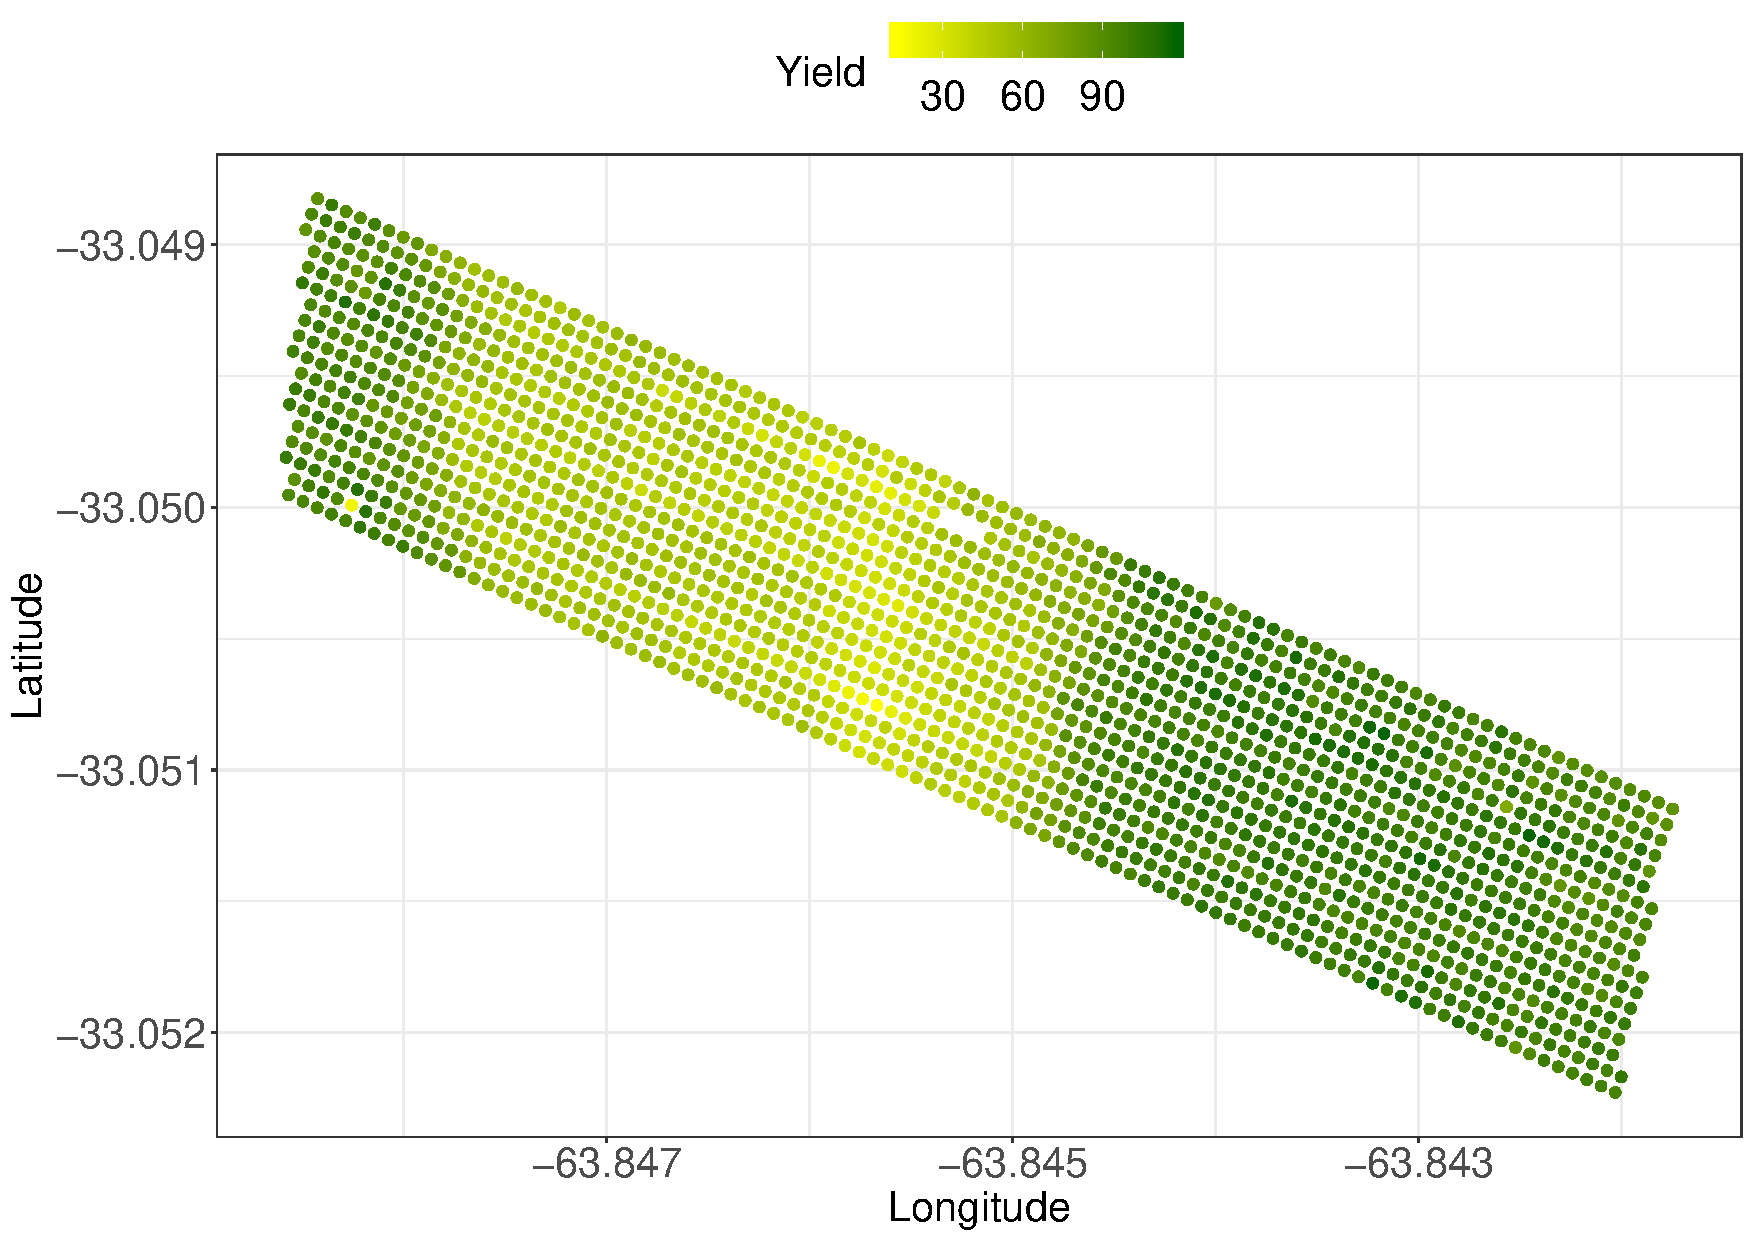
\includegraphics[height=6.3cm,width=\linewidth]{Images/lasrossa_view01}
			\caption{Visualisation of yield. Yellow colour indicates low yield and dark green indicates high yield.}\label{fig:lasrossayield}
		\end{subfigure}
		\space
		\begin{subfigure}[t]{0.45\textwidth}
			\centering
			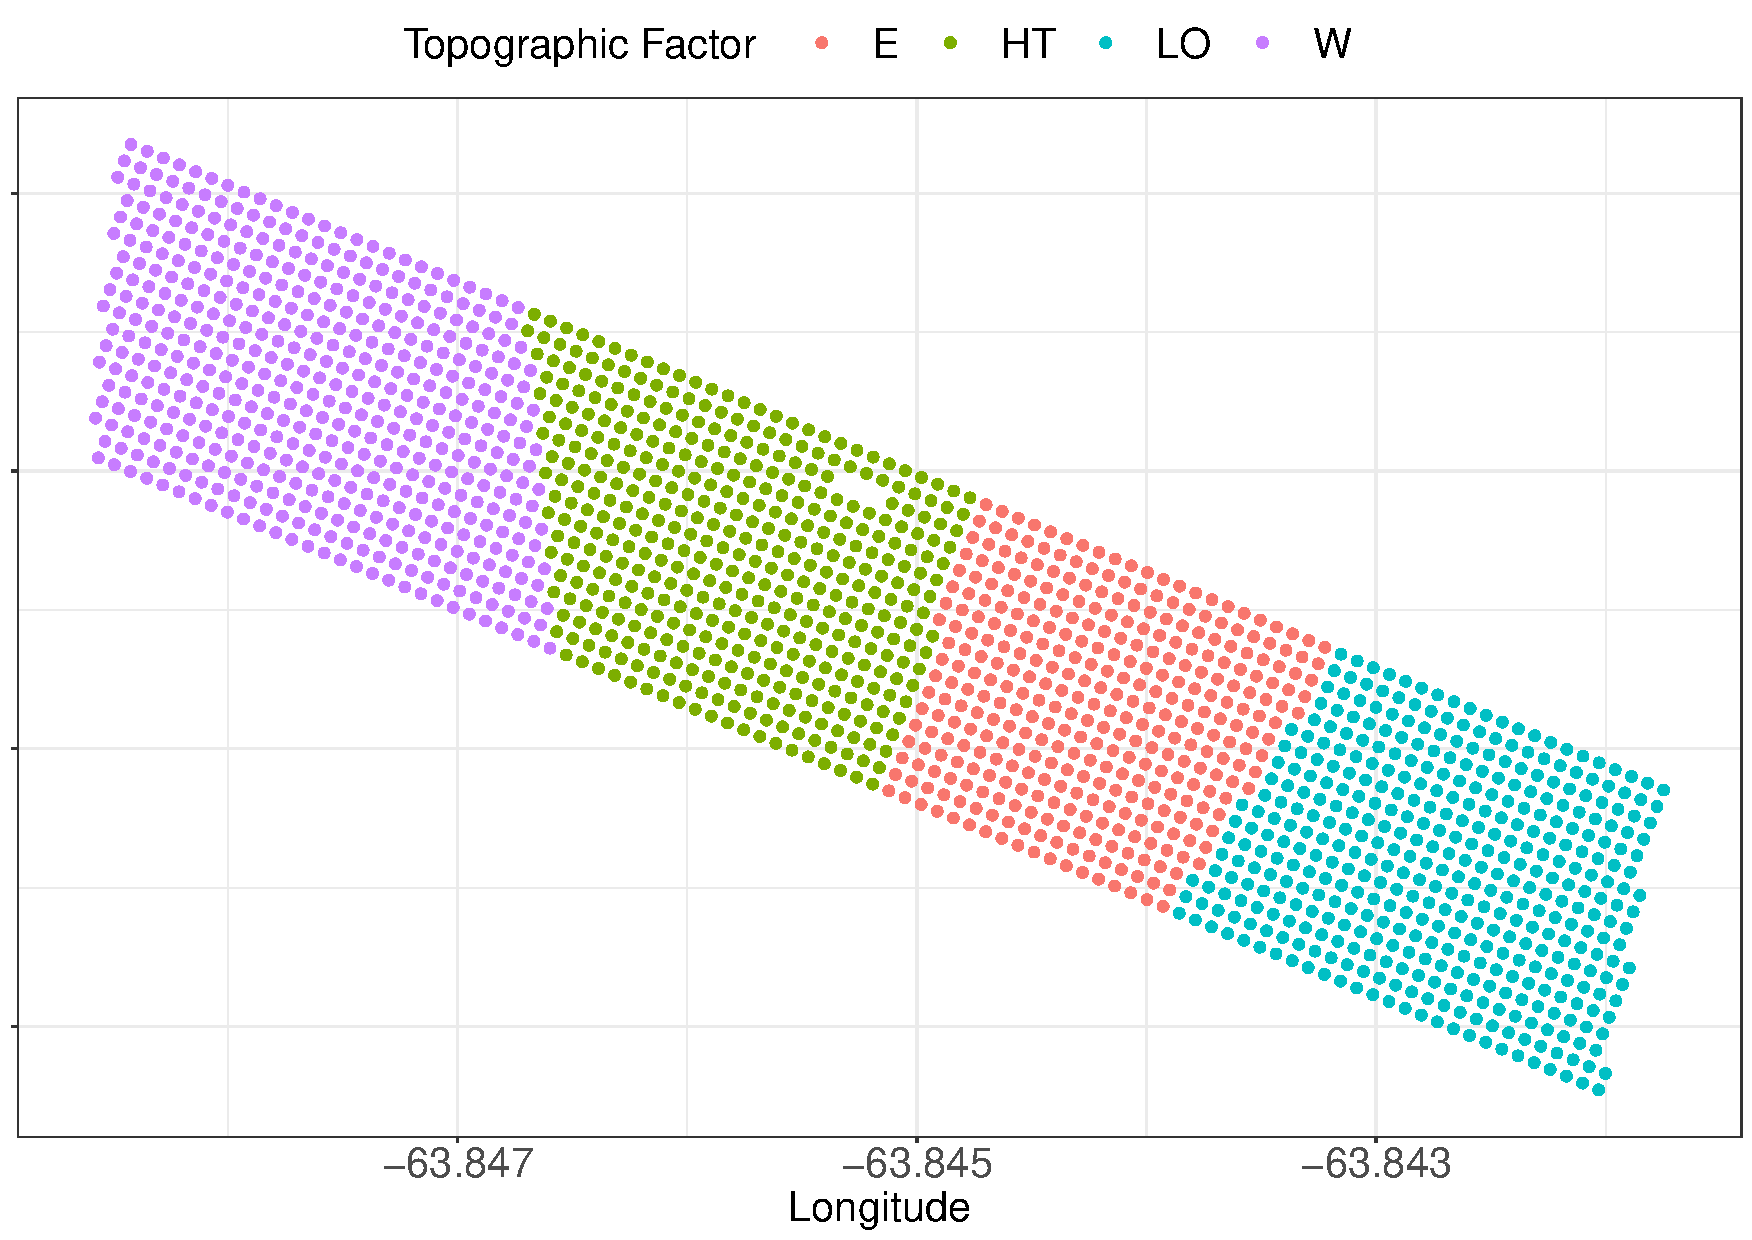
\includegraphics[height=6.0cm,width=0.9\linewidth]{Images/lasrossa_view02}
			\caption{Coloured by different topographic factors: West slope (W), Hilltop (HT), East slope (E) and Low East (LO).}\label{fig:lasrossascatter}
		\end{subfigure}
		\begin{subfigure}[t]{0.45\textwidth}
			\centering
			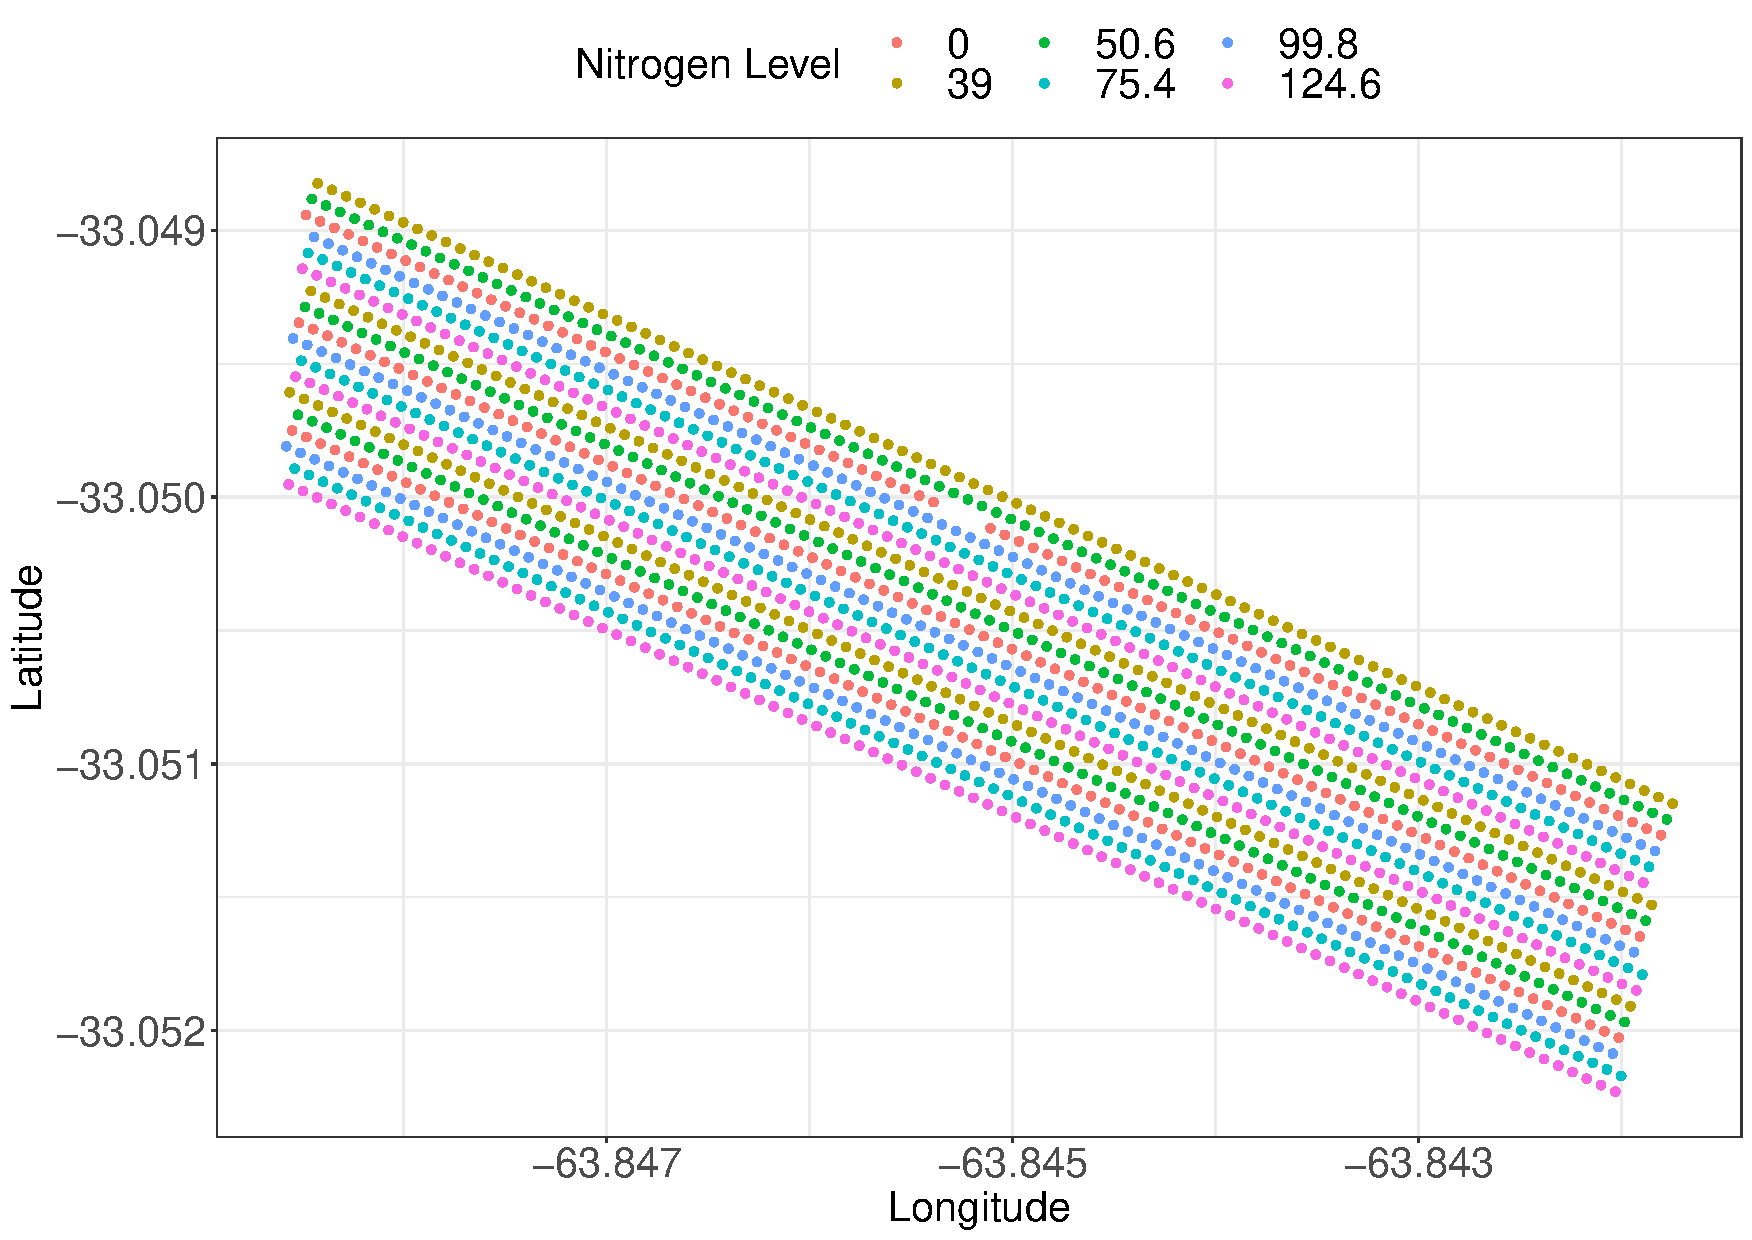
\includegraphics[height=6.3cm,width=\linewidth]{Images/lasrossa_view06}
			\caption{Six nitrogen treatment levels are systematically allocated into three replicates.}\label{fig:lasrossatopo}
		\end{subfigure}
		\space
% 		\begin{subfigure}[t]{0.45\textwidth}
% 			\centering
% 			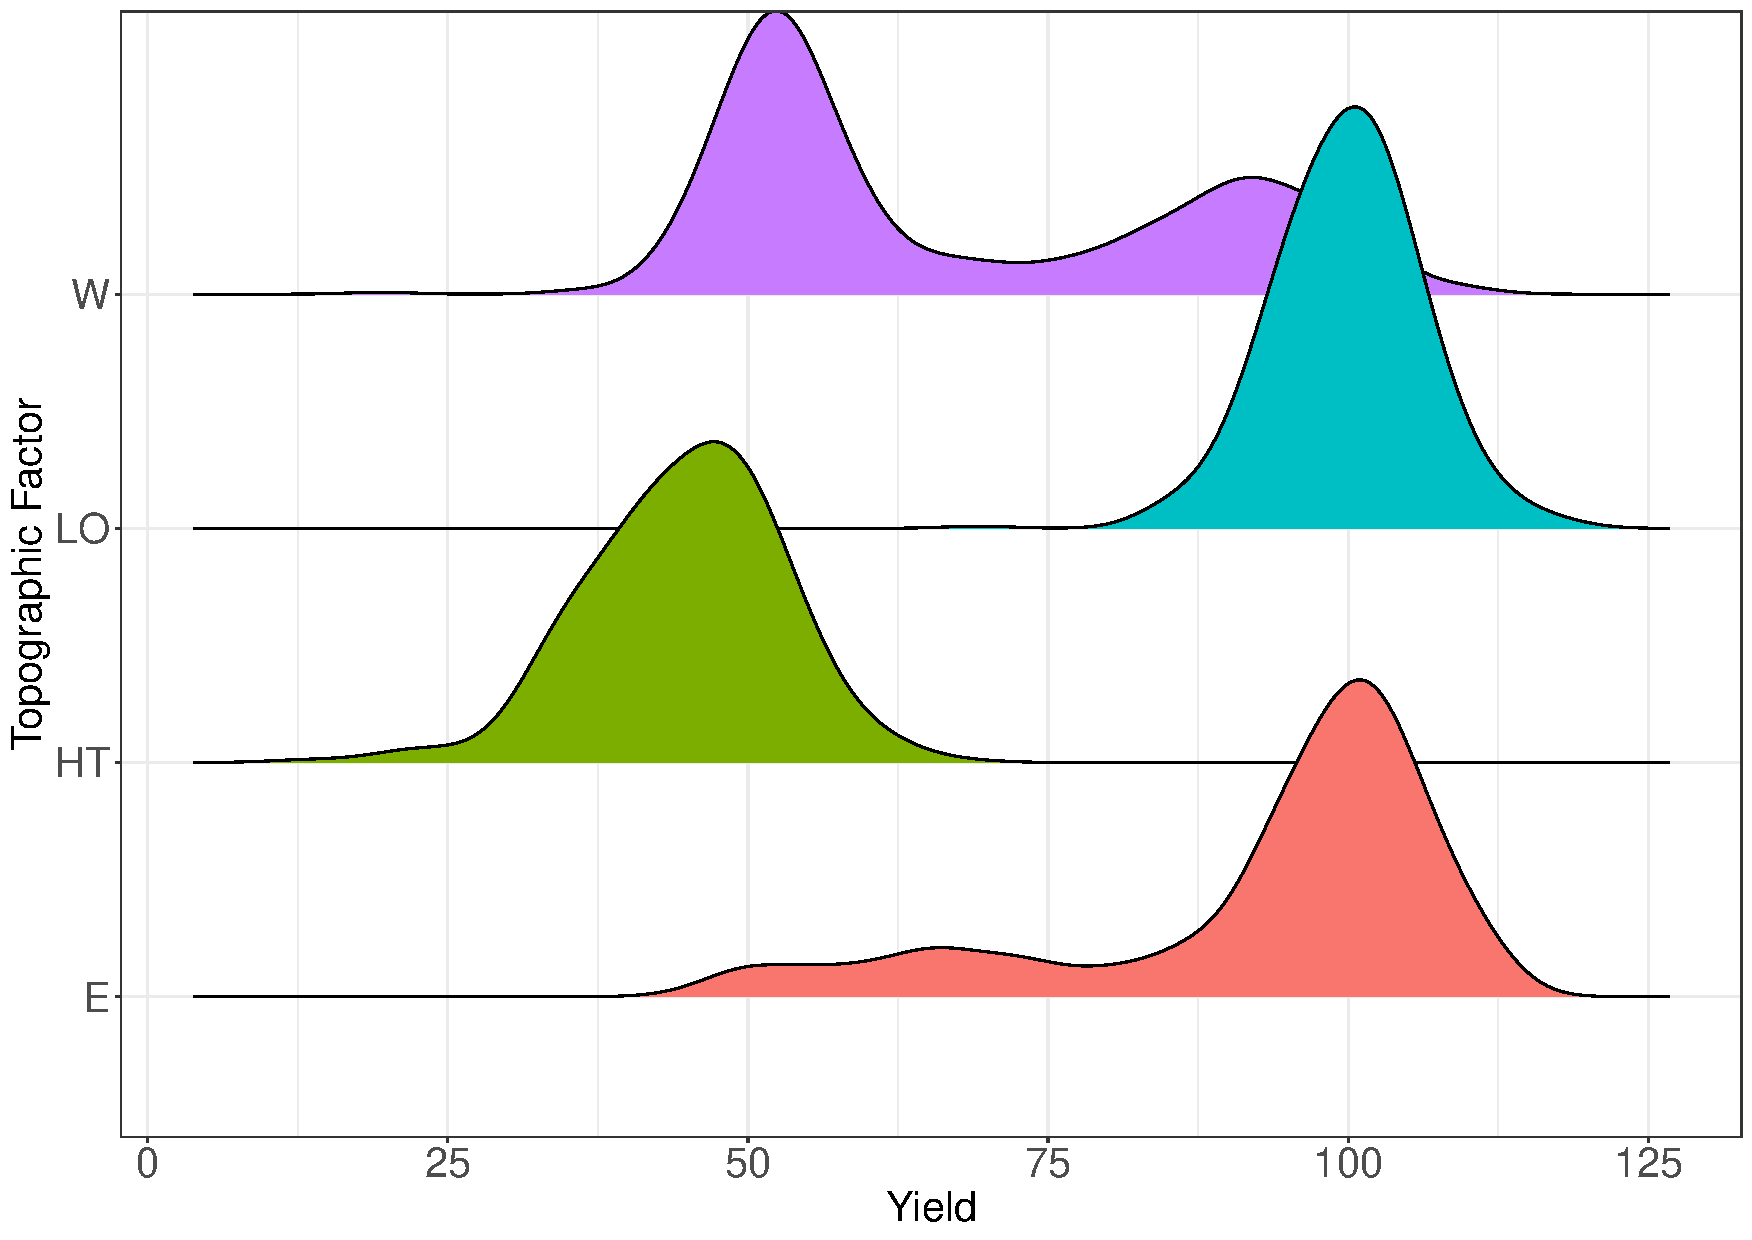
\includegraphics[height=6.3cm]{Images/lasrossa_view03}
% 			\caption{Histogram of yield by different topographic factors: West slope (W), Hilltop (HT), East slope (E) and Low East (LO).}\label{fig:lasrossascatter}
% 		\end{subfigure}
% 		\begin{subfigure}[t]{0.45\textwidth}
% 			\centering
% 			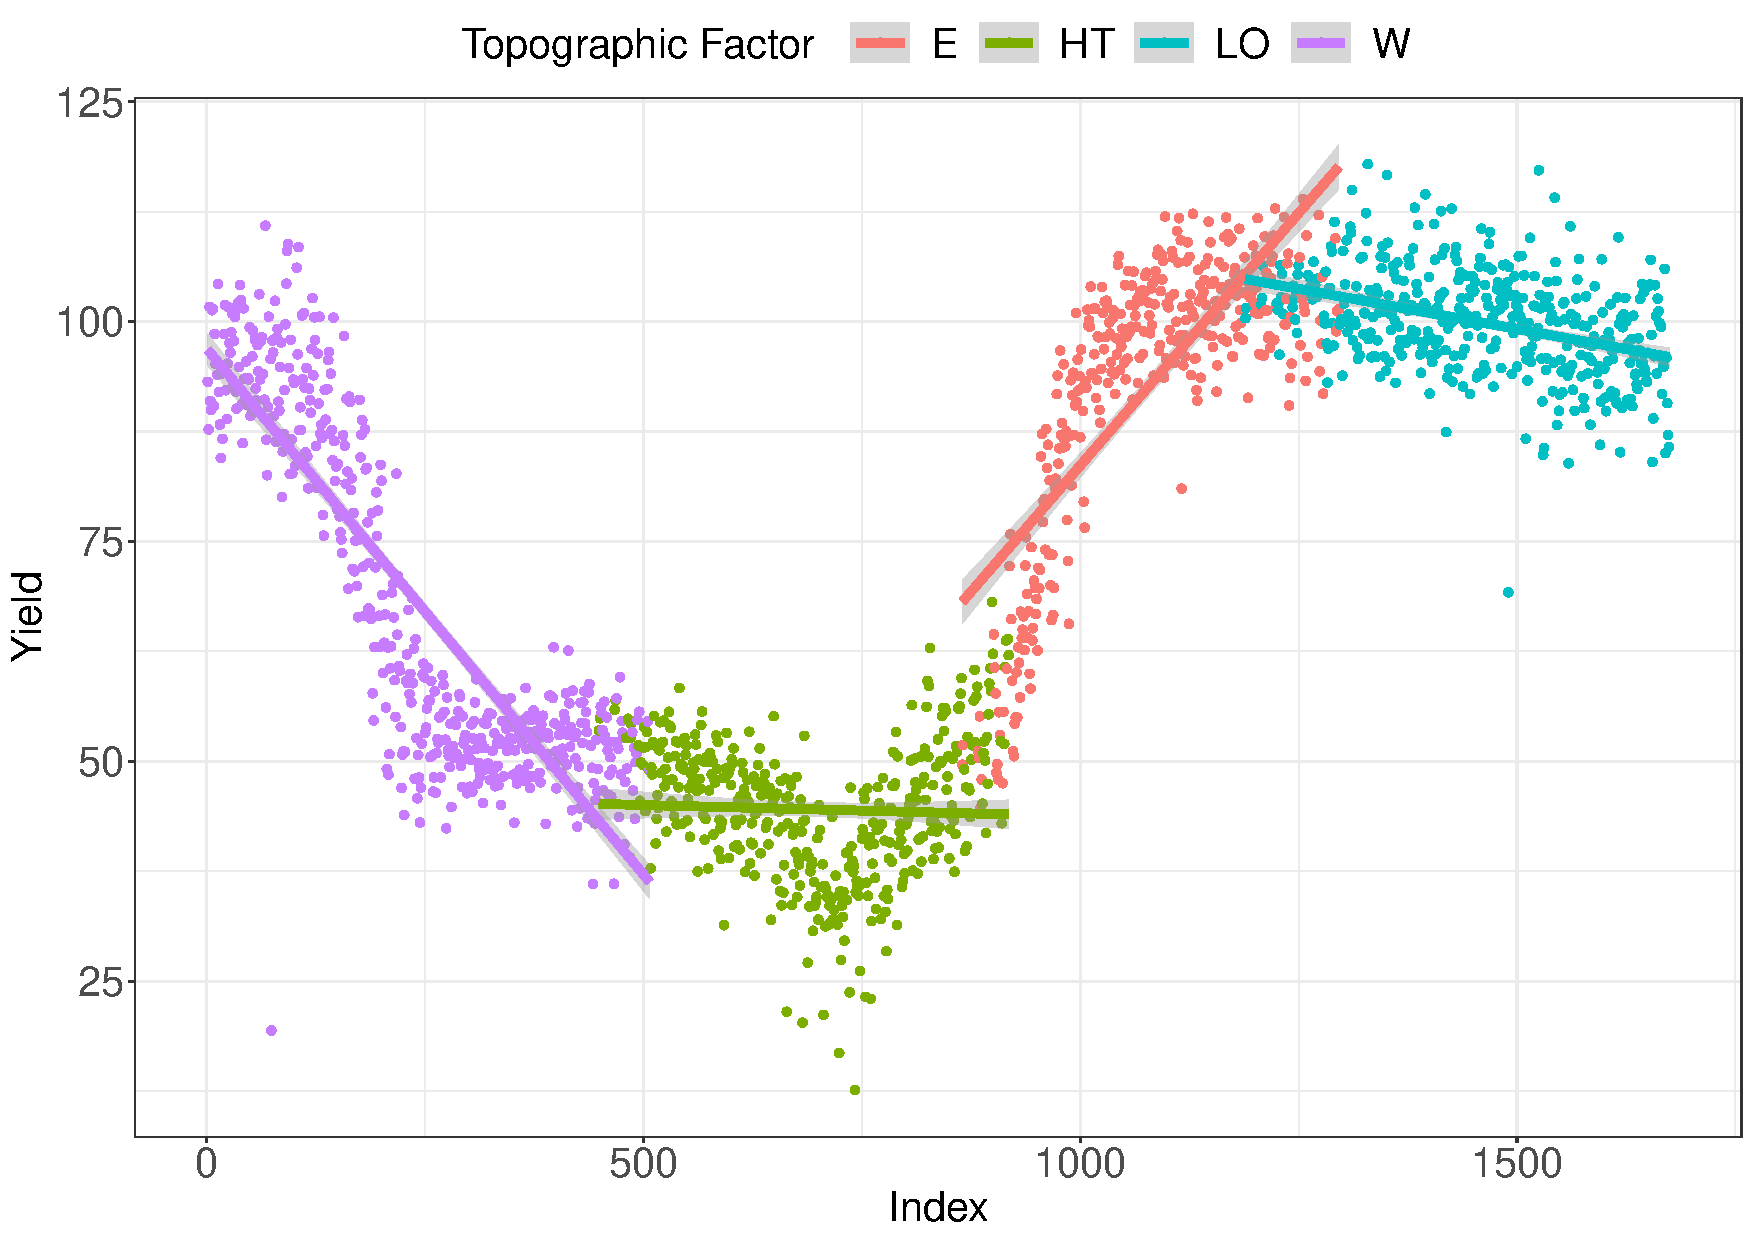
\includegraphics[height=6.3cm,width=\linewidth]{Images/lasrossa_view05}
% 			\caption{Linear models fitted within each topographic factor: West slope (W), Hilltop (HT), East slope (E) and Low East (LO).}\label{fig:lasrossascatter}
% 		\end{subfigure}
		%\space
		\begin{subfigure}[t]{0.45\textwidth}
			\centering
			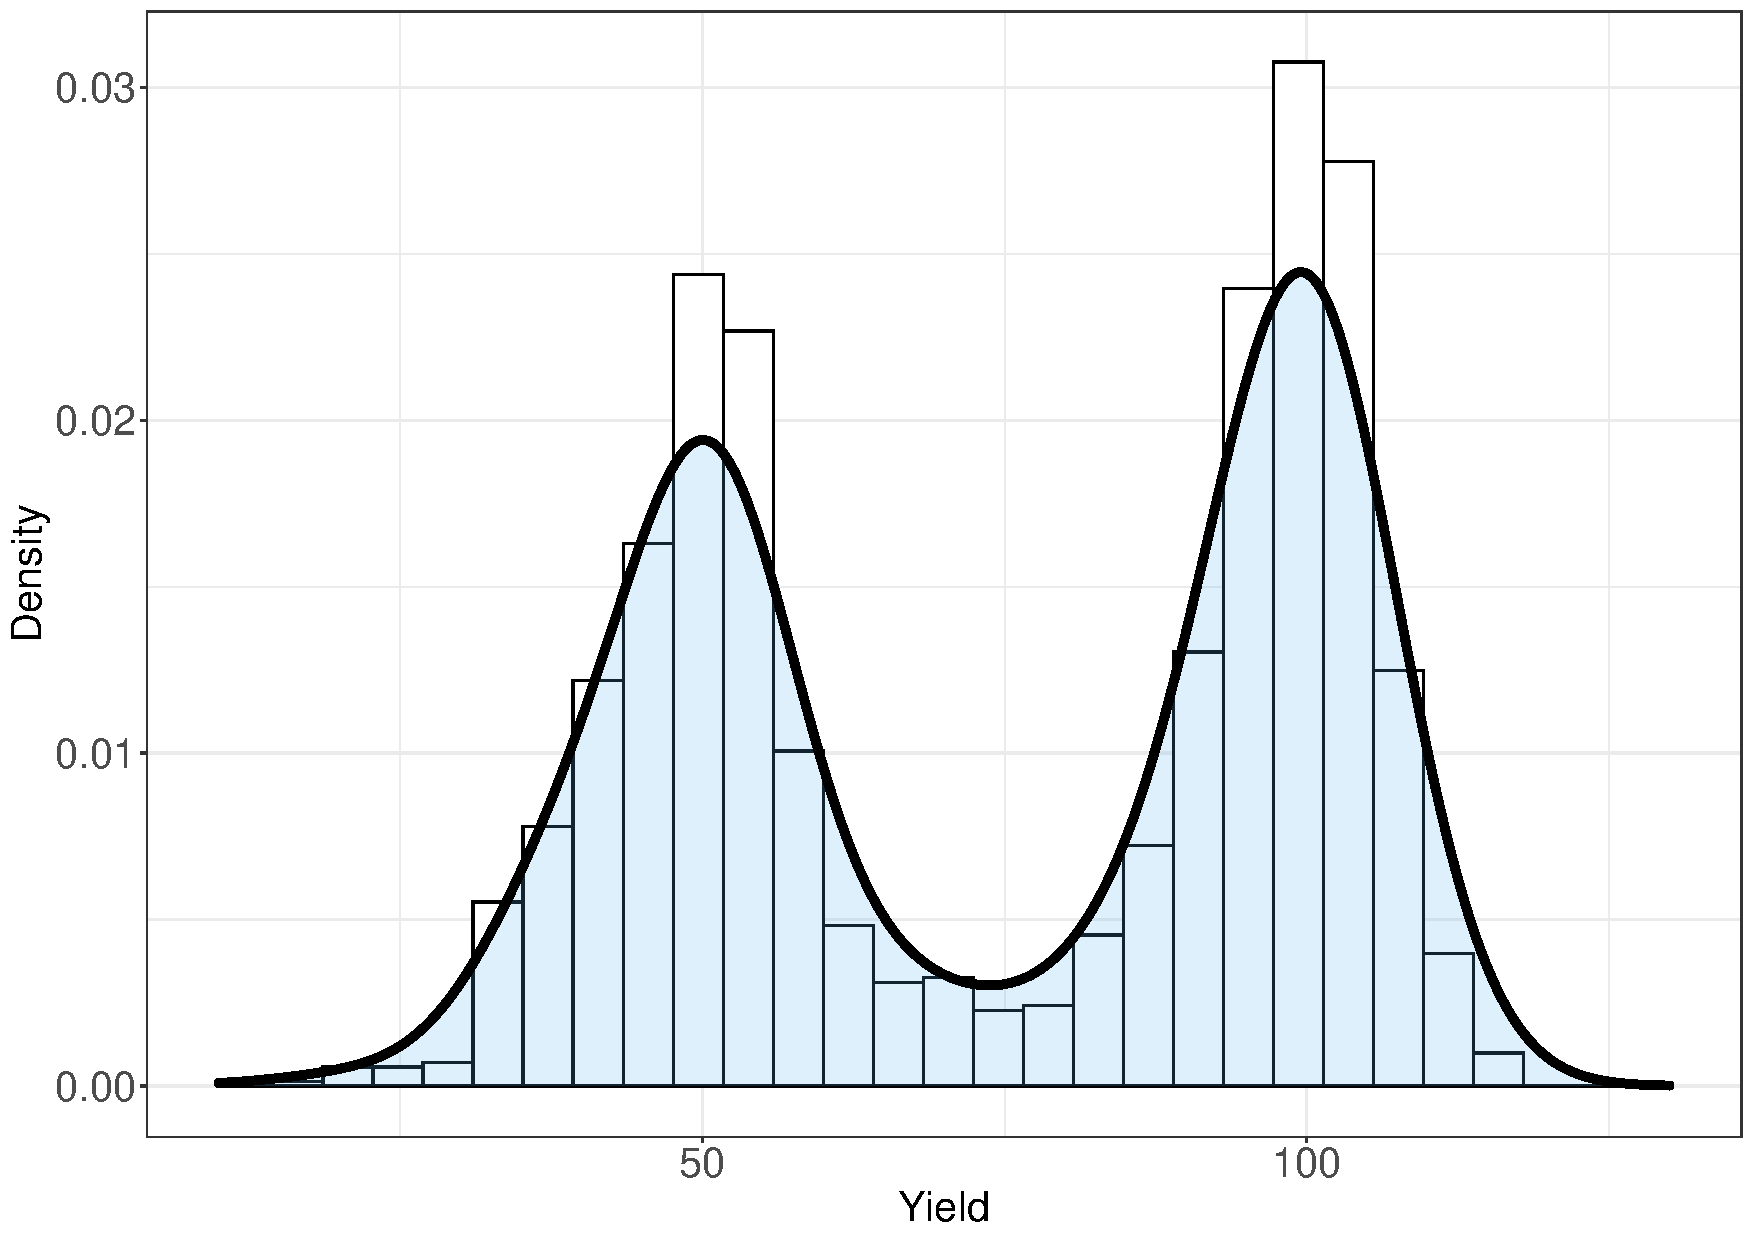
\includegraphics[height=5.7cm,width=\linewidth]{Images/lasrossa_view04}
			\caption{Bimodal histogram and density plot of yield.}\label{fig:lasrossahist}
		\end{subfigure}
		\caption{Visualisation of Las Rosas yield monitor data for harvests in 2001.}\label{fig:lasrossa}
	\end{figure}
	
	
	Additionally, a geographic projection was applied to the data. It transforms the geo-spatial coordinates to planar coordinates expressed in meters and assists with the model fitting \parencite{Rakshit2020Novel}. The field area of the Las Rosas experiment is approximately 810 metres long and 150 metres wide.
	
	
	
	\subsection{Statistical models and prior predictive simulations}
	
	\textcolor{red}{To obtain the map of locally varying optimal input rates, we specified a quadratic regression model, in which the corn yield is modelled as a quadratic function of the nitrogen rate. The optimal treatment can be determined by estimating the coefficients of the quadratic regression model at each grid point.} To demonstrate the flexibility of the proposed model \eqref{eq:underlying}, in which the random parameters $\bm{u}$ are spatially correlated, we compare it with the one without spatial correlation, used as a benchmark model for the rest of the analysis. We also compare two distributional assumptions in the context of specifying the likelihood -- the popular Gaussian likelihood has been compared with the Student-$t$ distribution in order to assess whether the  Gaussian model, often chosen as the default model, is misspecified for our example data set. We define our four models below in Table \ref{tb:models}. 
	
	
	\begin{table}[!htp]
		\centering
		\begin{tabular}{*{5}{l}} \toprule
			& Model 1 & Model 2& Model 3& Model 4  \\ \midrule
			Spatial correlation & No & Yes & No & Yes \\ 
			$\Var(\bm{u})$ &  $I_{n\times n}\otimes V_u$ & $V_s\otimes V_u$ & $I_{n\times n}\otimes V_u$ & $V_s\otimes V_u$ \\ 
			Distribution & Gaussian & Gaussian & Student-$t$ & Student-$t$ \\
			\bottomrule
		\end{tabular}\caption{Four models that are fitted in our study.}\label{tb:models}
	\end{table}
	
	
	The modelling process starts by selecting appropriate priors for the model parameters by comparing the simulated responses and the observed responses graphically, as shown in Figure~\ref{fig:priorcheck}. In the right panel of Figure~\ref{fig:priorcheck}, we have chosen weakly informative priors to simulate responses based on the quadratic regression function. In the left panel, we show the simulated responses obtained using vague priors for the regression coefficients.
	
	The vague priors used in our analysis are $b_0\sim \N(\mu,100)$, $b_1,b_2\sim \N(0,100)$ and $\sigma_e\sim IG(1,100)$, where $\mu$ is the median of the observed responses and $IG$ refers to the inverse Gamma distribution. We assume $u_{i_h}\sim \N(0,\sigma_{h}^2)$ with $\sigma_h^2\sim IG(1,100)$ and $h=0, 1, 2$ at grid $s_i$.  Alternatively, we can choose weakly informative priors $b_0\sim \N(80,10)$, $b_1\sim \N(0,0.01)$, $b_2\sim \N(0,0.001)$, $\sigma_{0}\sim \N_+(0,1)$, $\sigma_{1}\sim \N_+(0,0.01)$, $\sigma_{2}\sim \N_+(0,0.001)$, $R_u\sim \mbox{LKJcorr}(1)$ and $\sigma_e\sim \N_+(0,1)$, where $\N_+(\cdot)$ is the positive half Gaussian distribution. 
	
	The  correlation matrix $R_u$, defined in \eqref{eq:varmat}, is given by
	\begin{equation}\label{eq:RMat}
		R_u = \begin{bmatrix}
			1 & \rho_{12} &\rho_{13}  \\ \rho_{21} & 1 & \rho_{23} \\ \rho_{31} & \rho_{32} & 1 
		\end{bmatrix},
	\end{equation}
	where $\rho$s are the pairwise correlation parameters. For the correlation matrix $R_u$, we select $\mbox{LKJcorr}(\epsilon)$ with $\epsilon = 1$, which represents weak correlation amongst $\bm{u}_i$ values at grid $i$, $i=1,\ldots, n$.  
	
	Figure \ref{fig:LKJdensity} demonstrates how the distribution of $\rho$ is influenced by $\epsilon$. A small $\epsilon$ leads to a wider tail and a big $\epsilon$ typically narrows down the tail. In the case of $\epsilon = 1$, all correlations are equally plausible. As $\epsilon$ increases, the variables are more likely to be independent. 
	
	\begin{figure}[!htp]
		\centering	
		\begin{subfigure}[t]{0.45\textwidth}
			\centering
			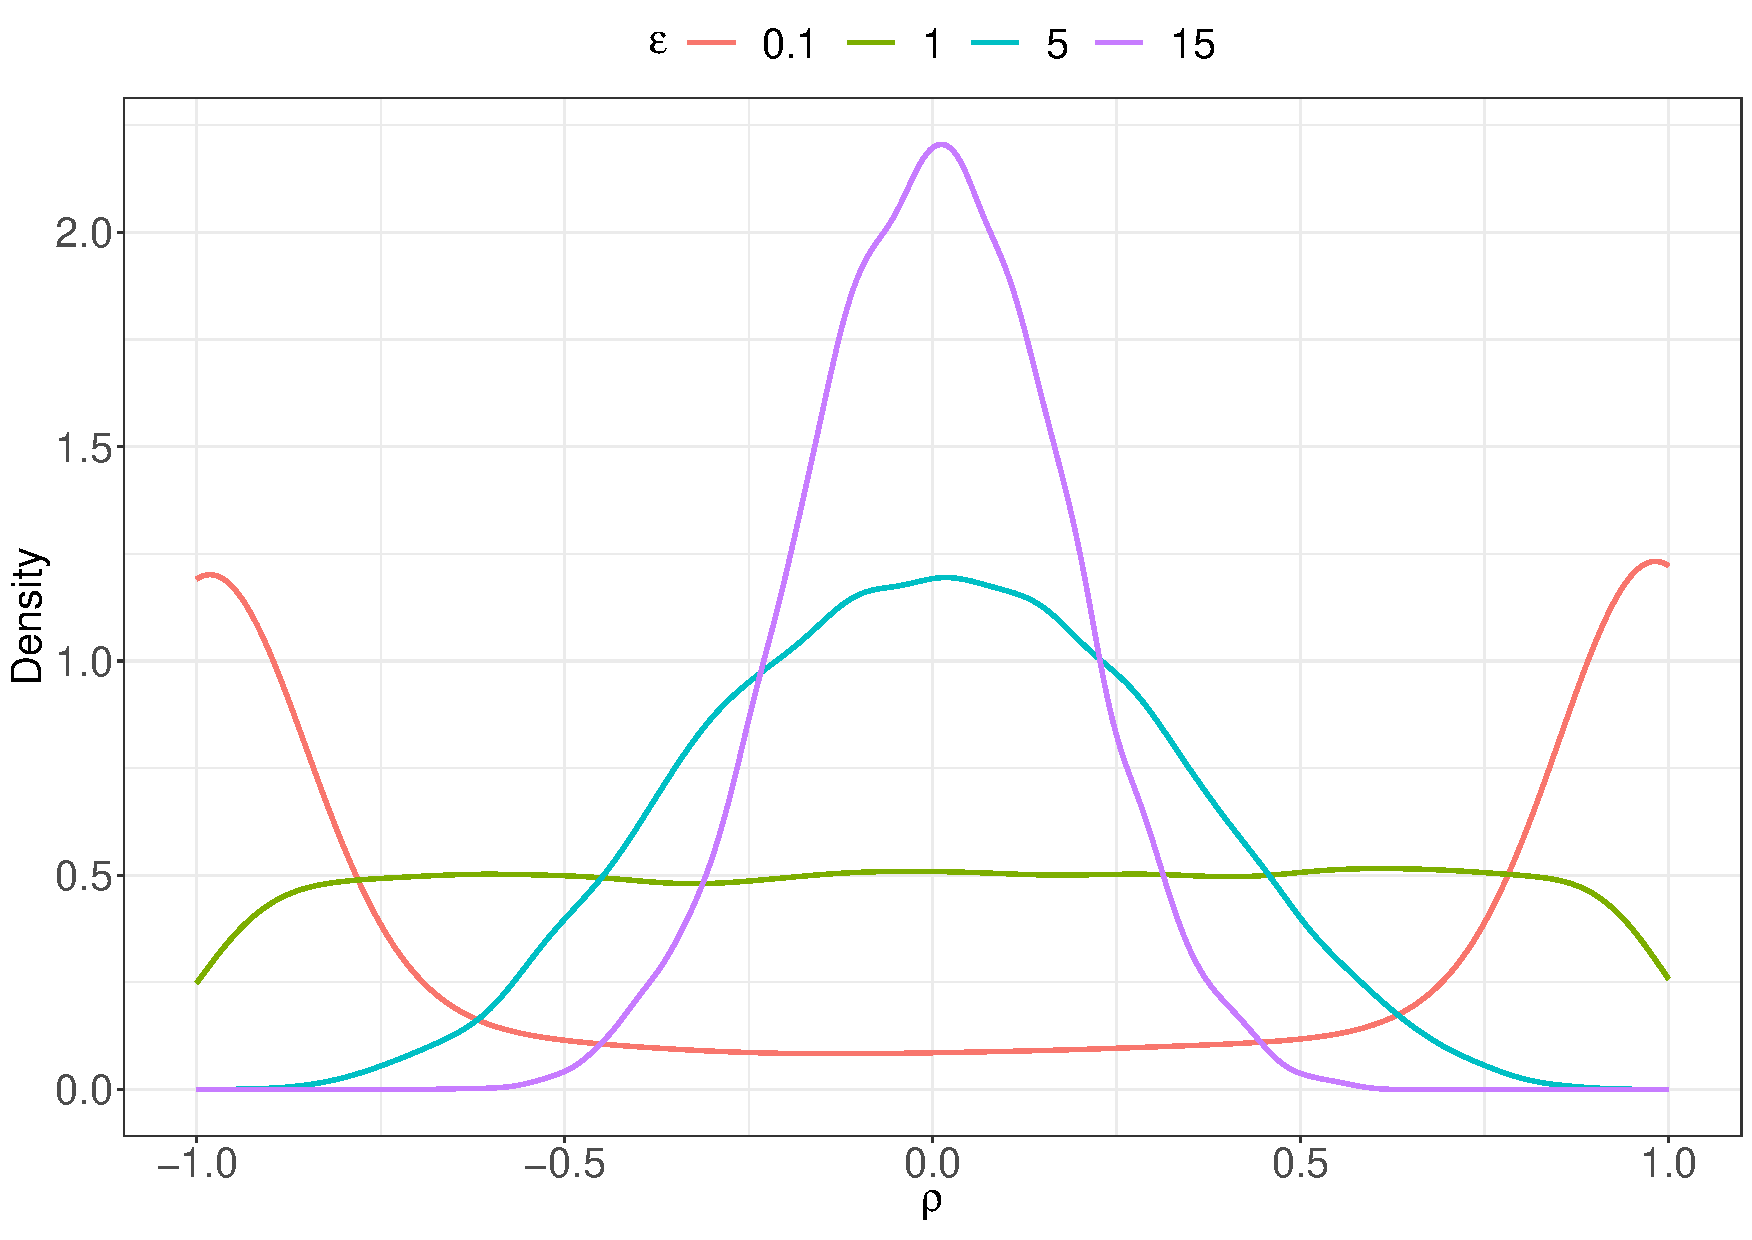
\includegraphics[height=6.3cm,width=\linewidth]{Images/LKJdensity}
			\caption{Distribution of correlation coefficients $\rho$ extracted from random $2\times2$ correlation matrices with different values of $\epsilon$.}
		\end{subfigure} 
		\space
		\begin{subfigure}[t]{0.45\textwidth}
			\centering
			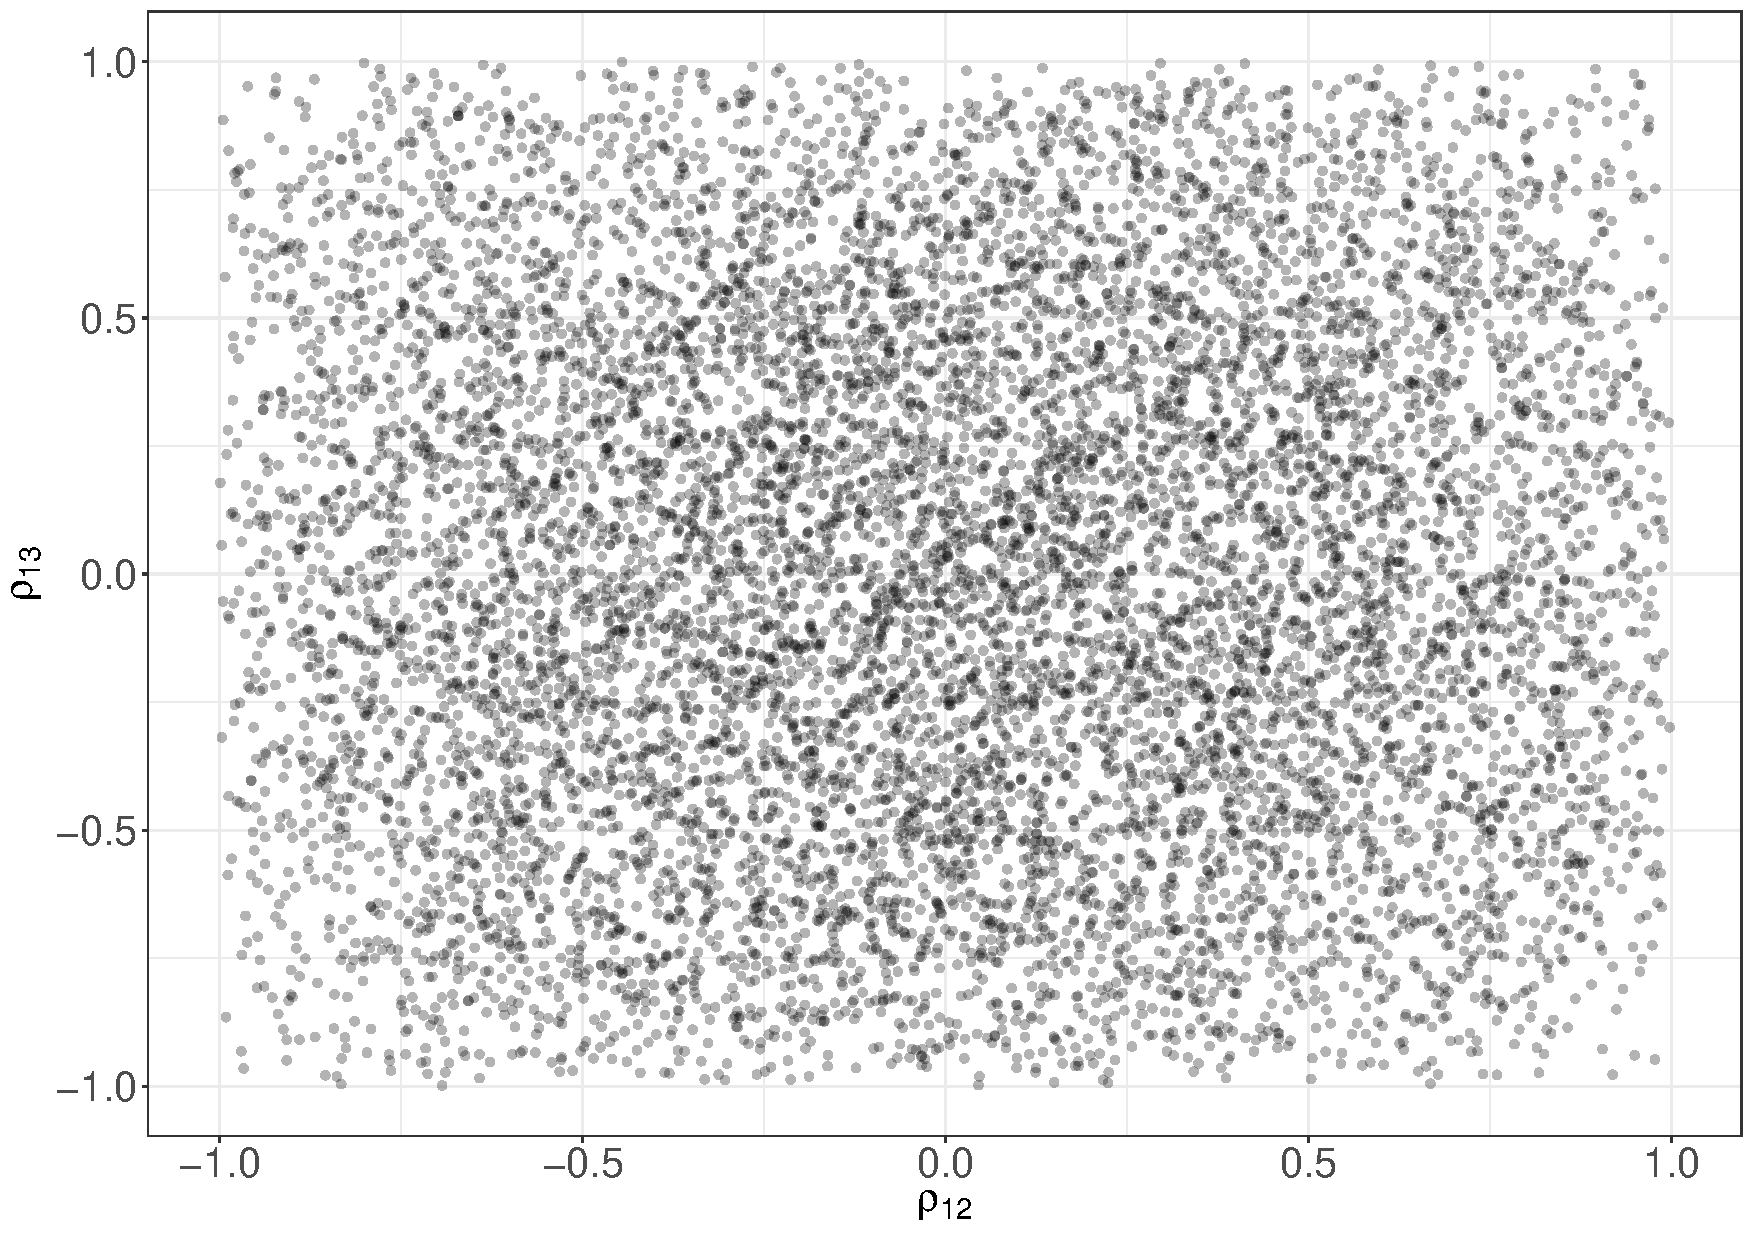
\includegraphics[height=5.9cm,width=\linewidth]{Images/LKJdensity2D}
			\caption{Visualisation of $\rho_{12}$ against $\rho_{13}$ from a $3\times3$ correlation matrix with $\epsilon=1$.}
		\end{subfigure}
		\caption{$\text{LKJcorr}(\epsilon)$ probability density. }\label{fig:LKJdensity}
	\end{figure}
	
	
	
	
	Figure \ref{fig:priorcheck} compares the simulated data with vague and weakly informative priors. When the vague priors are applied, Model 1 generates extremely small and large values, which are highly unlikely for our corn yield data set. This is mostly because the vague priors disregard practical knowledge. The use of weakly informative priors avoids negative values and keeps the simulations within a reasonable interval. Even though some simulations are not perfect, the weakly informative priors overall exhibit good results that reflect commonsense knowledge about the yield response. On the other hand, if the priors are too informative, the posterior distribution maybe badly influenced and result in partial exploration of the posterior space. 
	
	%where $t$ is the Student-$t$ distribution in the form
	%\begin{equation}
	%t(y\mid\nu,\mu,\tau) = \frac{\Gamma((\nu+1)/2)}{\Gamma(\nu/2)}\frac{1}{\sqrt{\nu\pi}\tau} \left(1+\frac{1}{\nu}  \left(\frac{y-\mu}{\tau} \right)^2  \right)^{-(\nu+1)/2}
	%\end{equation}
	%for degrees of freedom $\nu$ and scale parameter $\tau\in\mathbb{R}^+$, mean $\mu$ and $y\in\mathbb{R}$, and $t(\cdot)^+$ indicate a positive half-$t$ distribution with given parameters. 
	
	\begin{figure}[!htp]
		\centering
		\begin{subfigure}[t]{0.45\textwidth}
			\centering
			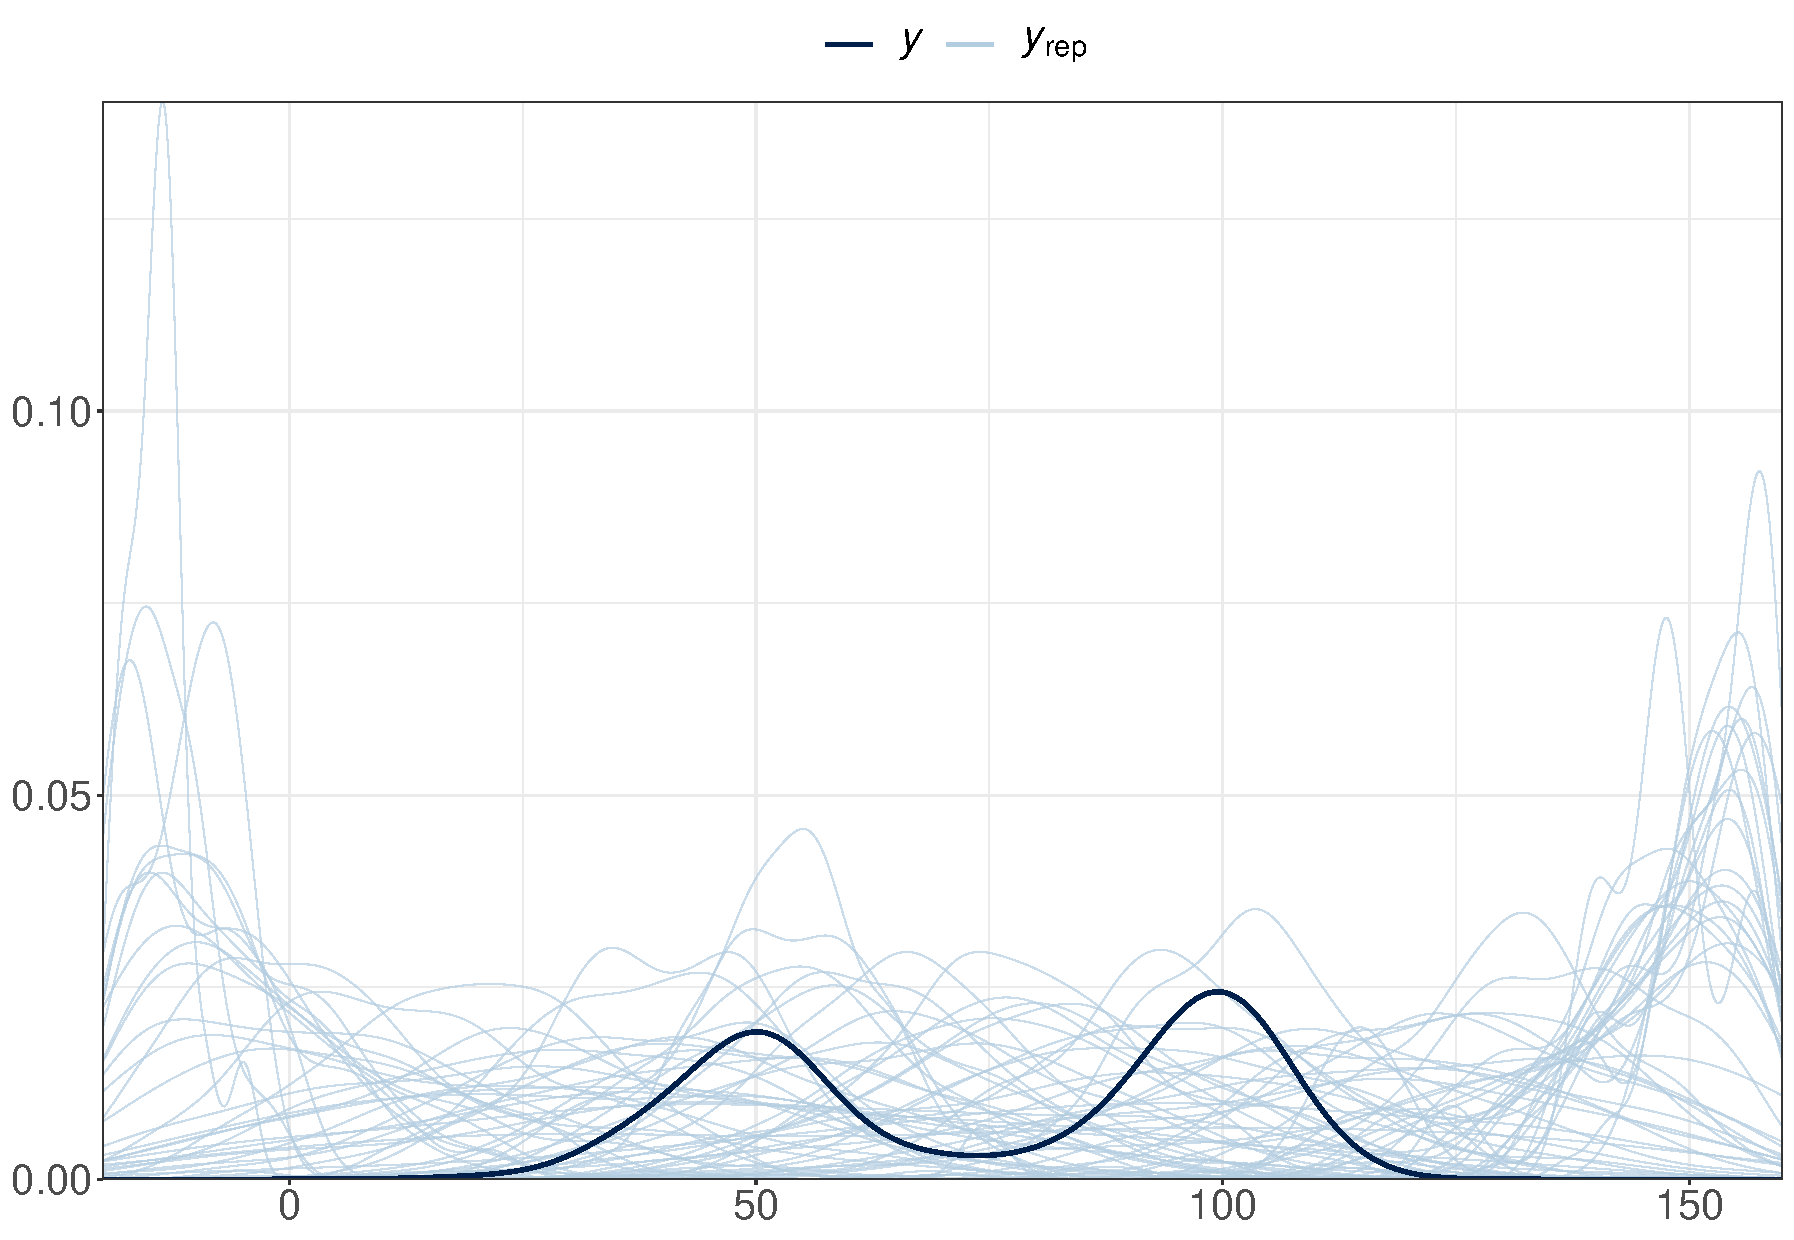
\includegraphics[width=\linewidth]{Images/priorcheck_vague}
			\caption{With vague priors}
		\end{subfigure}
		\space
		\begin{subfigure}[t]{0.45\textwidth}
			\centering
			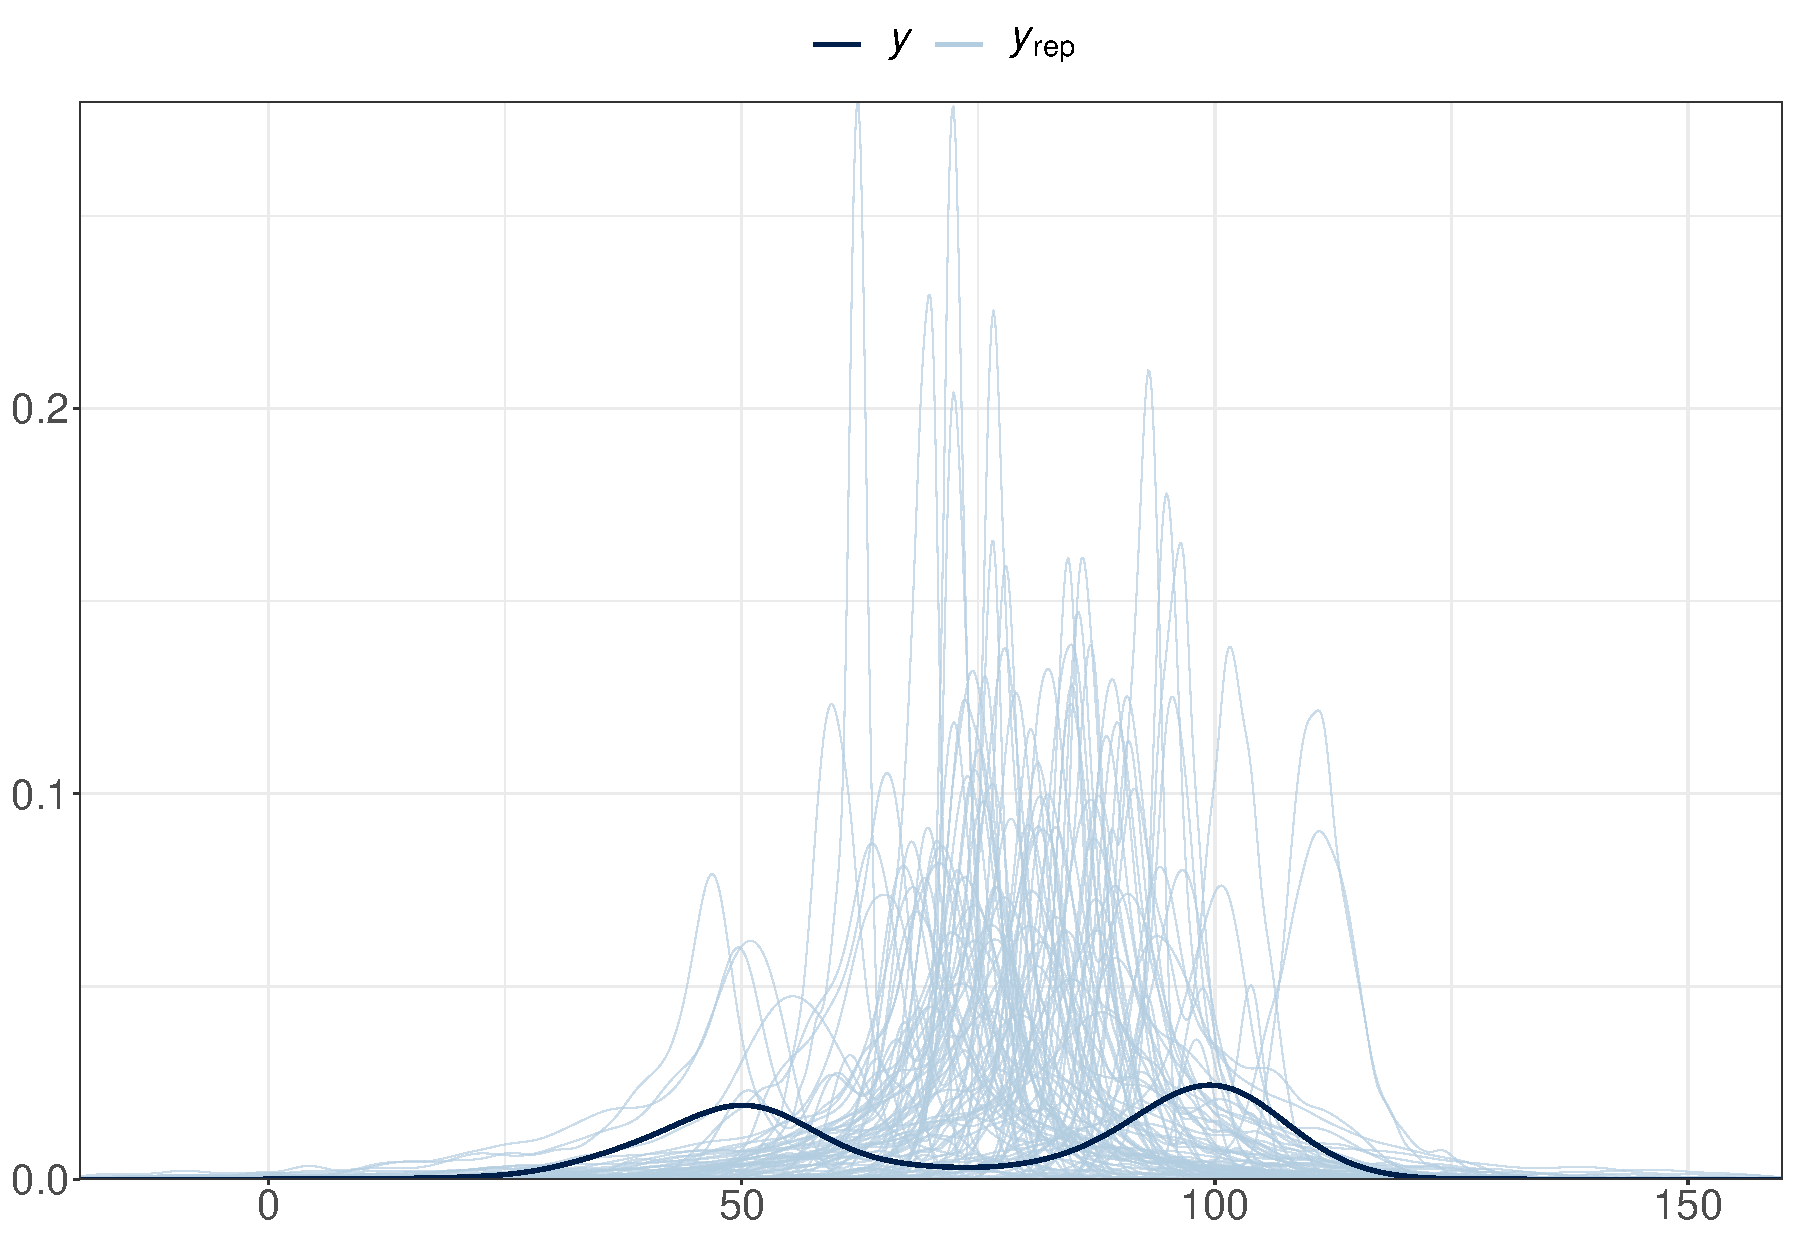
\includegraphics[width=\linewidth]{Images/priorcheck_weak}
			\caption{With weakly informative priors}
		\end{subfigure}
		\caption{Capability of regenerating observed data with different priors by running 100 simulations. Vague priors failed in regenerating and lead to extreme values. Weakly informative priors give plausible regenerated data. }\label{fig:priorcheck}
	\end{figure}
	
	
	
	In Model 2, in addition to the priors used in Model 1, we need priors for the parameters $\rho_c$ and $\rho_r$, and suppose $\rho_c,\rho_r\sim U(0,1)$, where $U(0,1)$ is the uniform distribution between 0 and 1. In Model 3 and 4, we have an extra parameter $\nu(\geq 1)$ for the degrees of freedom, and we specify a Gamma prior $\nu\sim \Gamma(2,0.1)$, as suggested by \textcite{Juarez2010ModelBased}. 
	
	In Table \ref{tb:priors}, we present the complete list of priors selected for our study. In general, it is not recommended to use the same priors across all the different models listed in Table \ref{tb:priors}. Furthermore, if a new prior is proposed for a new parameter, examining the suitability of that prior is recommended for each model. In this study, we have checked the suitability of all the priors for all our four models, and it turns out that the same priors, listed in the top-half of Table~\ref{tb:priors}, work well for all the four models (see Figure~\ref{fig:priorcheck4models} for further details). Consequently, we built the models by using the same weakly informative priors for a number of common parameters, and only adding new priors (listed in the bottom-half of Table~\ref{tb:priors}) for the additional parameters.
	
	
	%Additionally, NUTS does not require conjugate priors, which means the results are still valid if our priors are Gaussian but for the data Student-$t$ distribution is assumed. 
	
	
	\begin{table}[!htp]
		\centering
		\begin{tabular}{l *{4}{c}} \toprule
			& Model 1 & Model 2& Model 3& Model 4  \\ \midrule
			$b_0$ & \multicolumn{4}{c}{$\N(80, 10)$} \\ 
			$b_1$ & \multicolumn{4}{c}{$\N(0, 0.01)$} \\ 
			$b_2$ & \multicolumn{4}{c}{$\N(0, 0.001)$} \\ 
			$\sigma_0$ & \multicolumn{4}{c}{$\N_+(0, 1)$} \\ 
			$\sigma_1$ & \multicolumn{4}{c}{$\N_+(0, 0.01)$} \\
			$\sigma_2$ & \multicolumn{4}{c}{$\N_+(0, 0.001)$} \\ 
			$\sigma_e$ & \multicolumn{4}{c}{$\N_+(0, 1)$} \\ \midrule
			$R_u$ & --- & LKJcorr(1) & --- & LKJcorr(1) \\ 
			$\rho_c$ & --- & $U(0,1)$ & --- & $U(0,1)$ \\ 
			$\rho_r$ & --- & $U(0,1)$ & --- &  $U(0,1)$ \\ 		
			$\nu$ & --- &  --- & $\Gamma(2,0.1)$ & $\Gamma(2,0.1)$ \\ 
			\bottomrule
		\end{tabular}\caption{Priors of four models. Top-half: priors for common parameters of four models; Bottom-half: new priors for additional parameters.}\label{tb:priors}
	\end{table}
	
	Using the above priors, our proposed hierarchical Bayesian models were run on four parallel Markov chains using the \R-package \rstan\ with each chain having a warmup period of 1000 iterations and post-warmup period of another 1000 iterations. Consequently, for each parameter, we generated 4000 samples (1000 samples from each of the four chains) from its posterior distribution. 	
	
	\subsection{Posterior checking}\label{ss:PostCheck}
	
	The prior predictive checking is a powerful tool for understanding the structure of the model. However, it is not possible to extend this technique to choose between competing models for the data and evaluate their predictive performances. To assess the performance of a fitted model and diagnose potential model misspecifications, it is crucial to include posterior checking in the Bayesian modelling workflow. We use MCMC and PP diagnostic tools as part of our posterior checking. 	
	
	We start with the PP checking to visualise the performance of the four models described in Table~\ref{tb:models}. Figure \ref{fig:ppcheck} displays the results of the PP checking. It appears that if we do not take into account the spatial correlation of parameters $\bm{u}$ (e.g., Model 1 and 3), we are incapable of simulating the data that adequately capture the distribution of the observations. On the contrary, because Models 2 and 4 incorporate spatial correlation into modelling, we see simulation results that closely mimic the observed yield from the Las Rosas experiment. 	
	
	\begin{figure}[!htp]
		\centering
		\begin{subfigure}[t]{0.45\textwidth}
			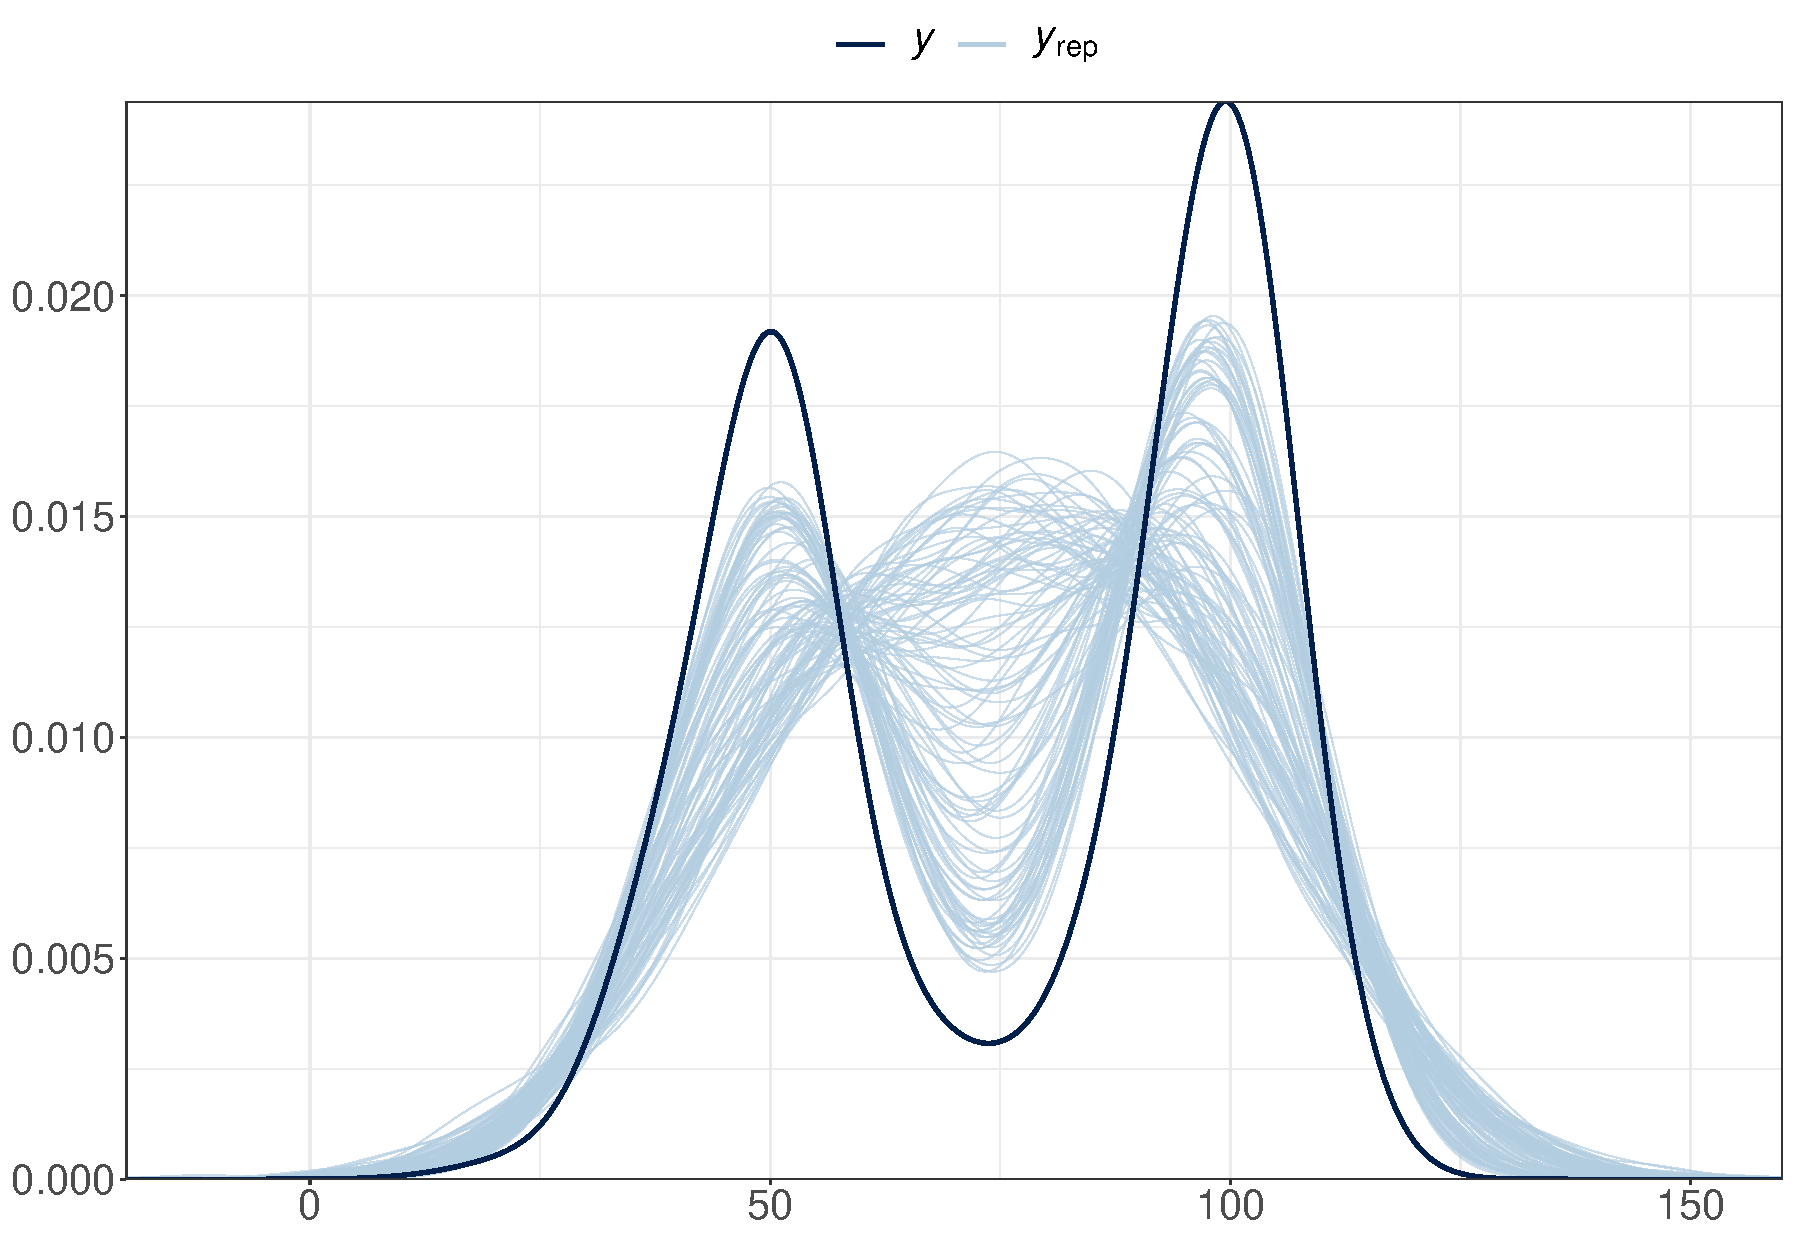
\includegraphics[width=\linewidth]{Images/ppcheck_GSRNS}
			\caption{PP check of Model 1}
		\end{subfigure}
		\begin{subfigure}[t]{0.45\textwidth}
			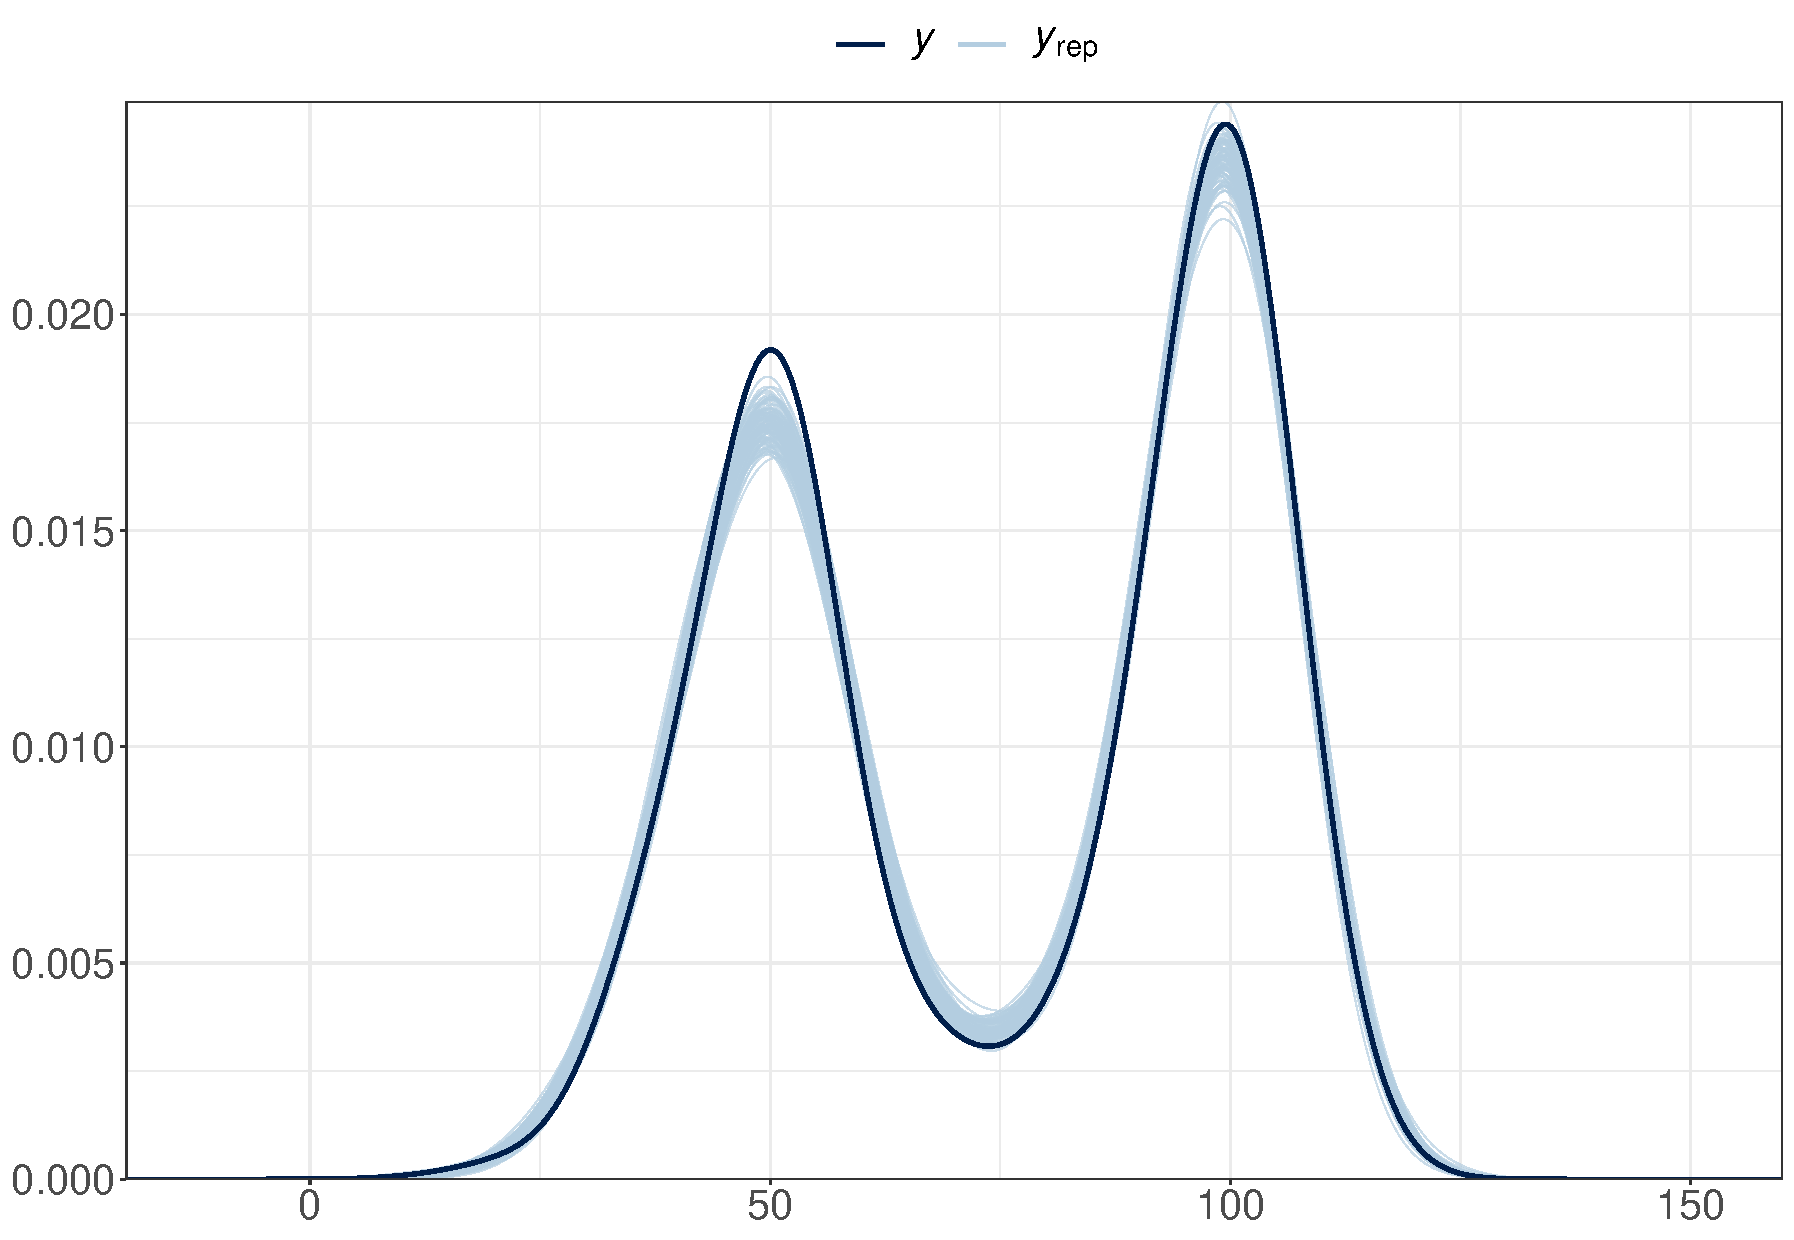
\includegraphics[width=\linewidth]{Images/ppcheck_GSRand}
			\caption{PP check of Model 2}
		\end{subfigure}
		\begin{subfigure}[t]{0.45\textwidth}
			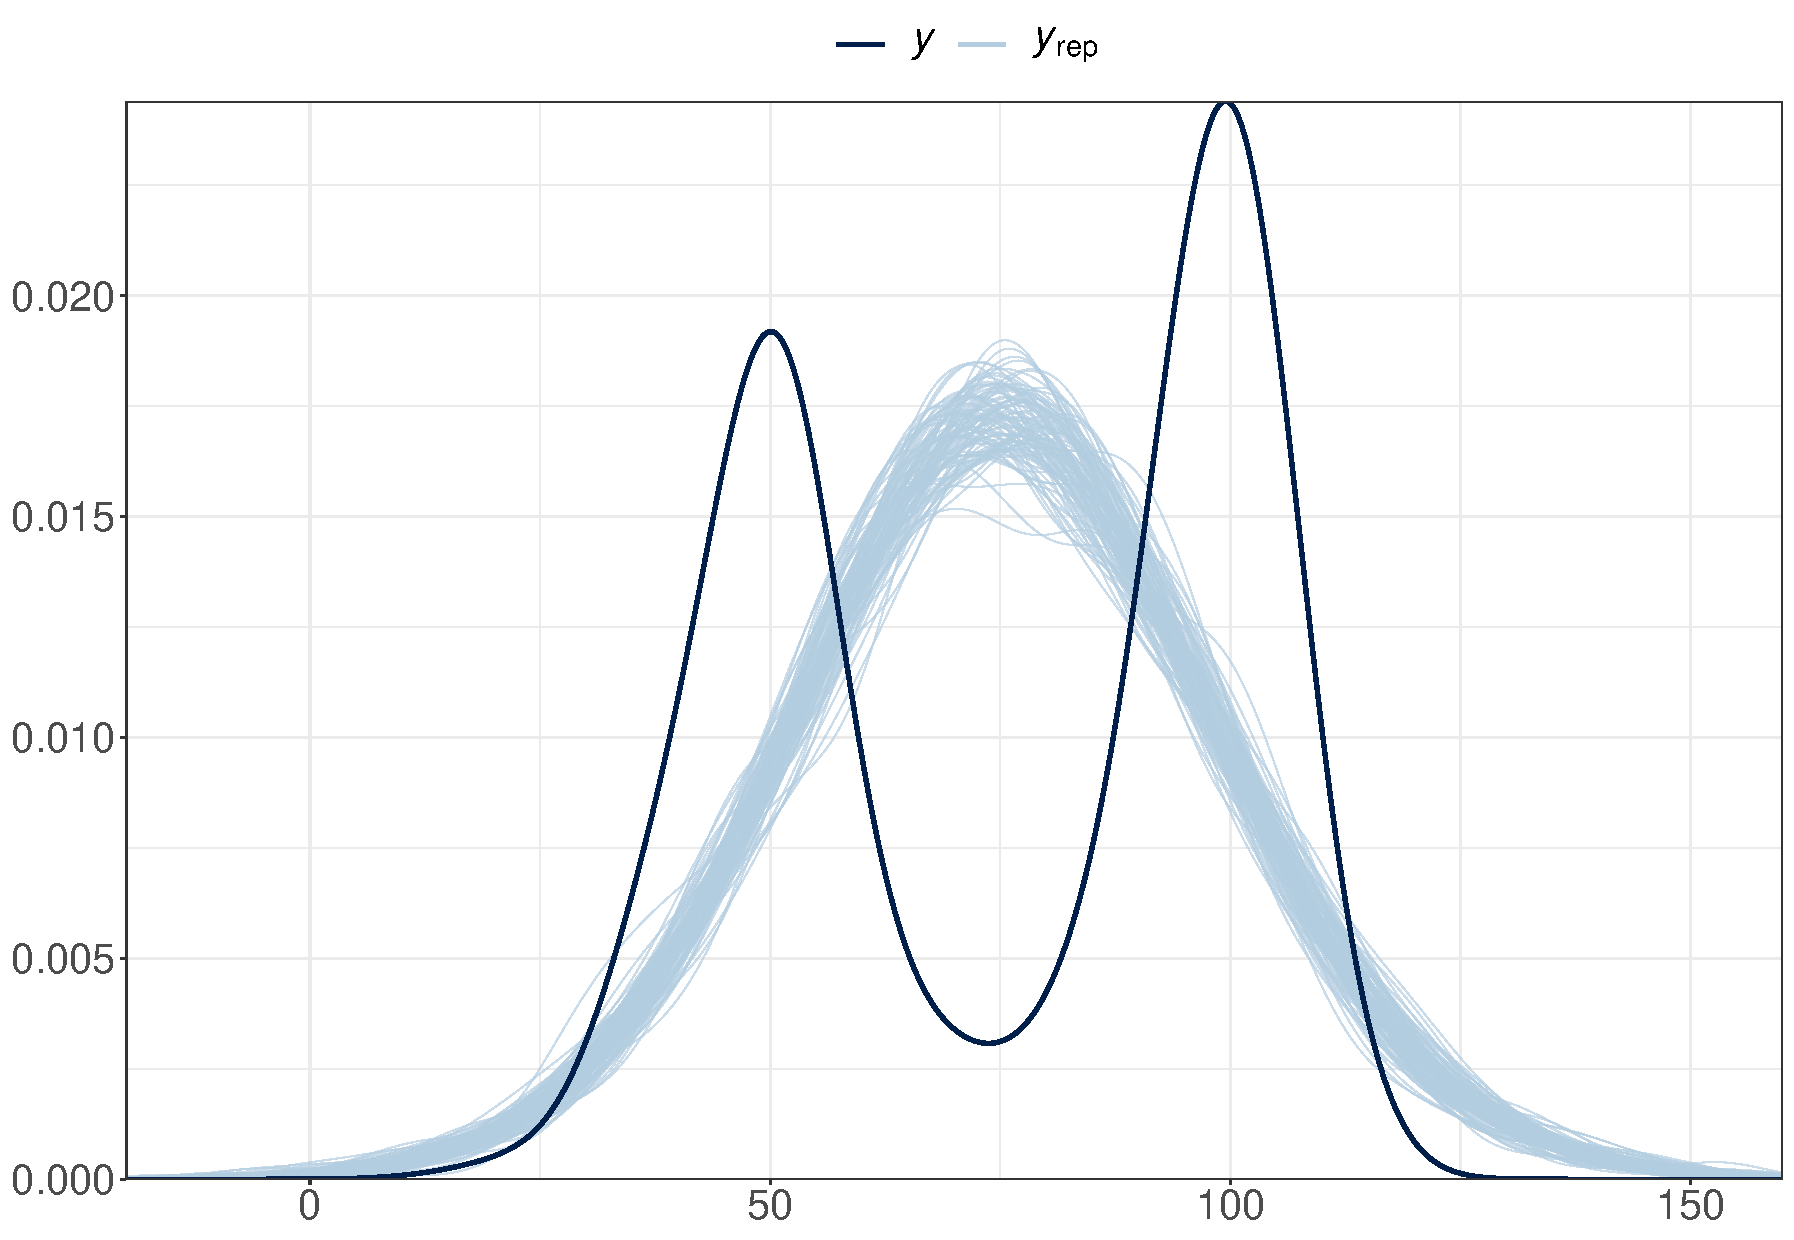
\includegraphics[width=\linewidth]{Images/ppcheck_STRNS}
			\caption{PP check of Model 3}
		\end{subfigure}
		\begin{subfigure}[t]{0.45\textwidth}
			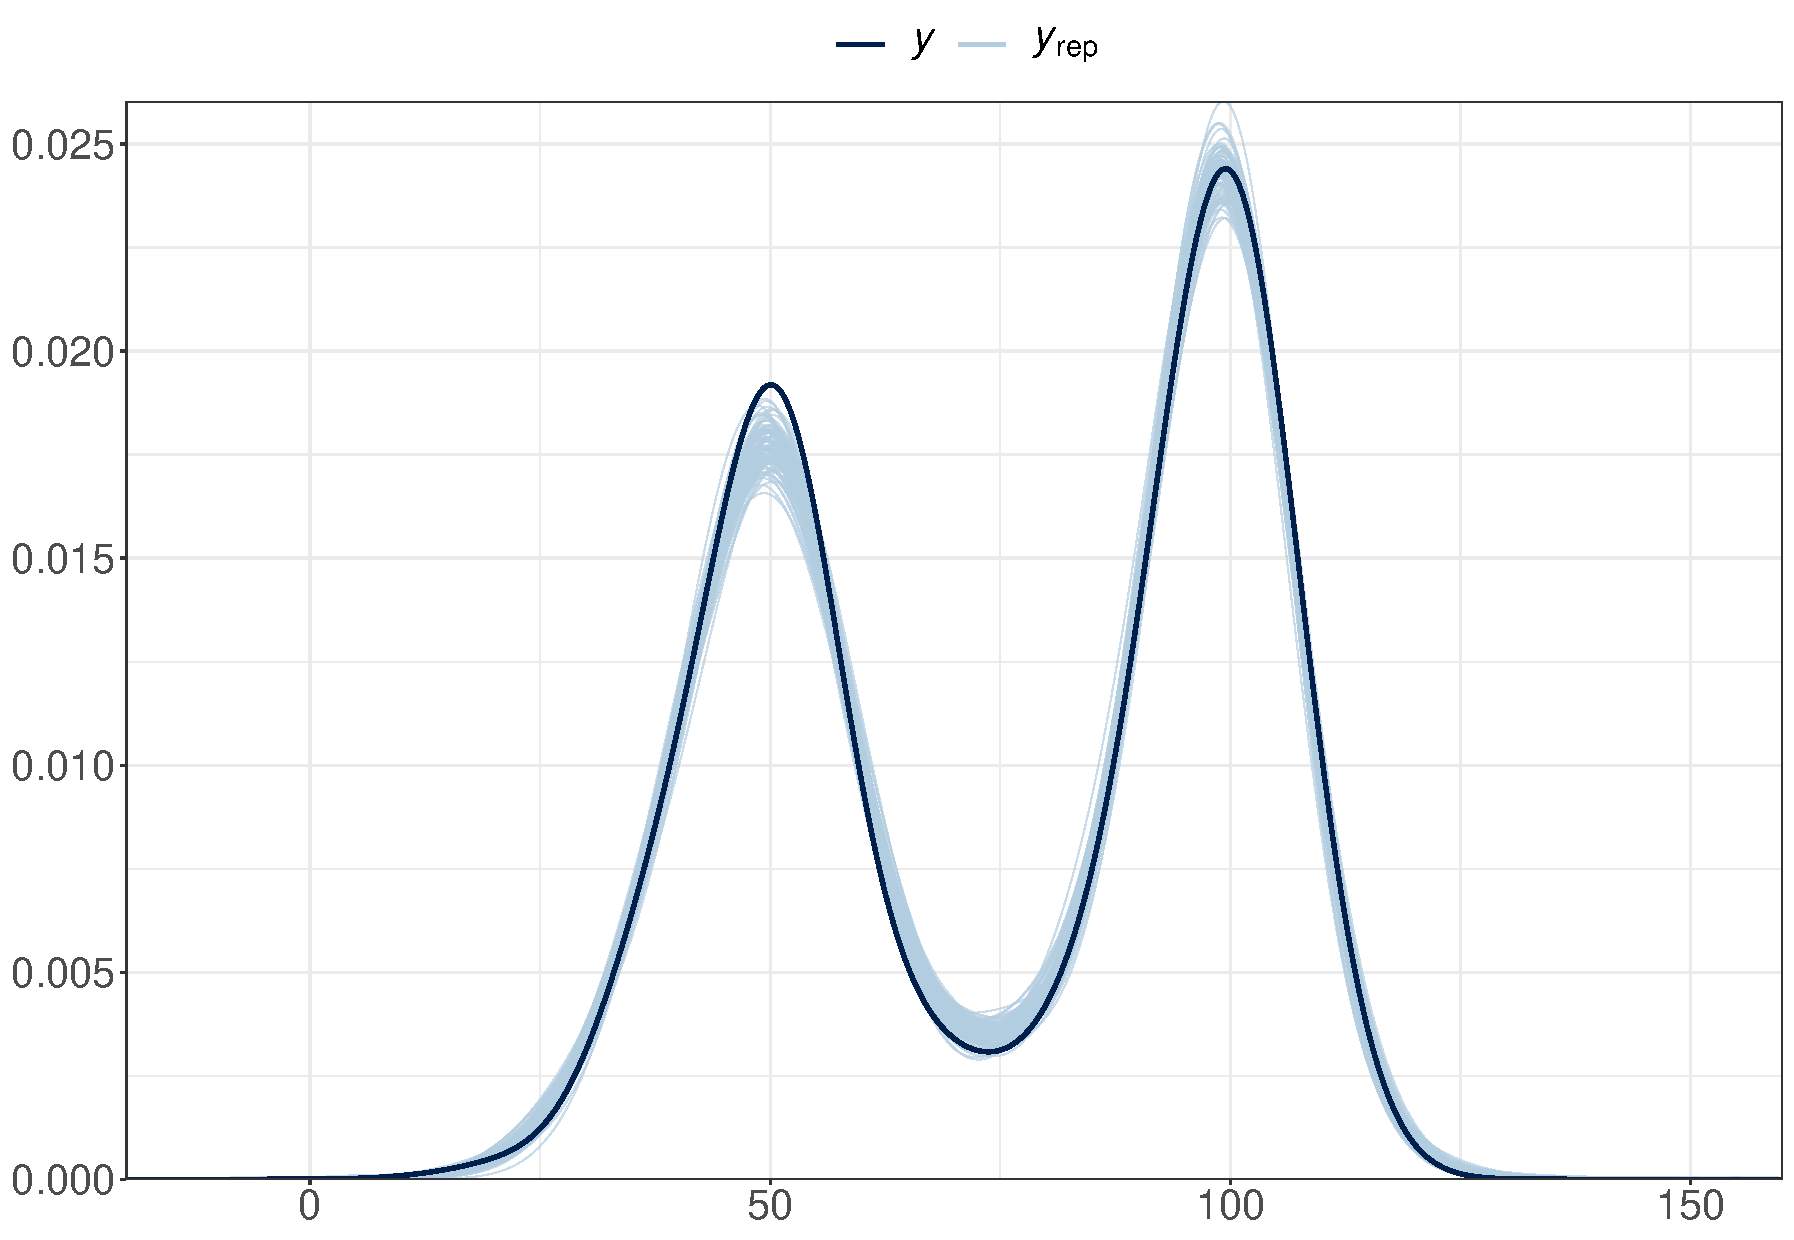
\includegraphics[width=\linewidth]{Images/ppcheck_STRand}
			\caption{PP check of Model 4}
		\end{subfigure}
		\caption{Posterior predictive checking for simple linear and the proposed spatial models with 100 simulations (blue lines) comparing to the observed data (black line).}\label{fig:ppcheck}
	\end{figure}
	
	
	Figure \ref{fig:skewcheck} illustrates the observed skewness of the posterior predictive distribution for the four models. While Model 2 and 4 capture the observed skewness, Model 1 and 3 demonstrate model misspecification. 
	
	\begin{figure}[!htp]
		\centering
		\begin{subfigure}[t]{0.45\textwidth}
			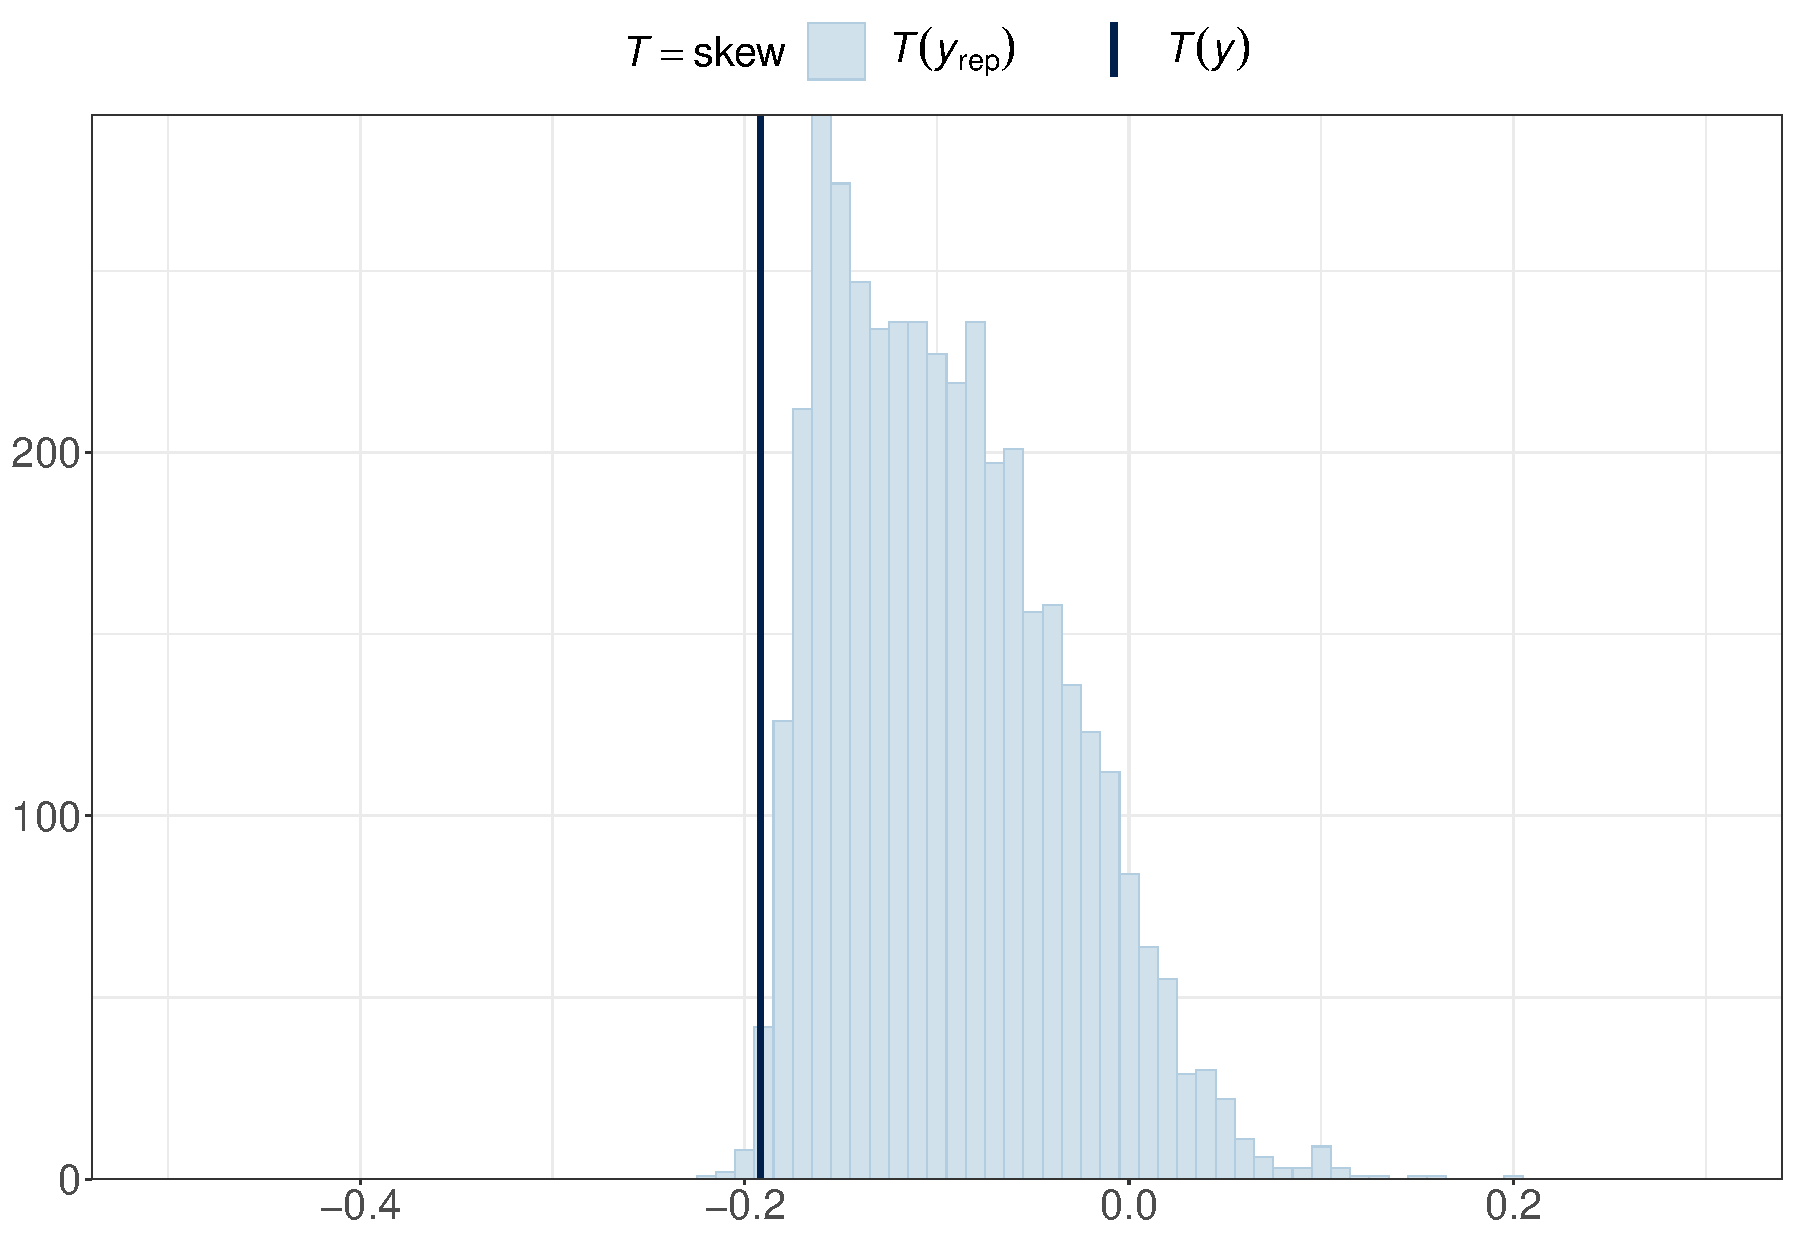
\includegraphics[width=\linewidth]{Images/skew_GSRNS_scale.pdf}
			\caption{Skew check of Model 1}
		\end{subfigure}
		\begin{subfigure}[t]{0.45\textwidth}
			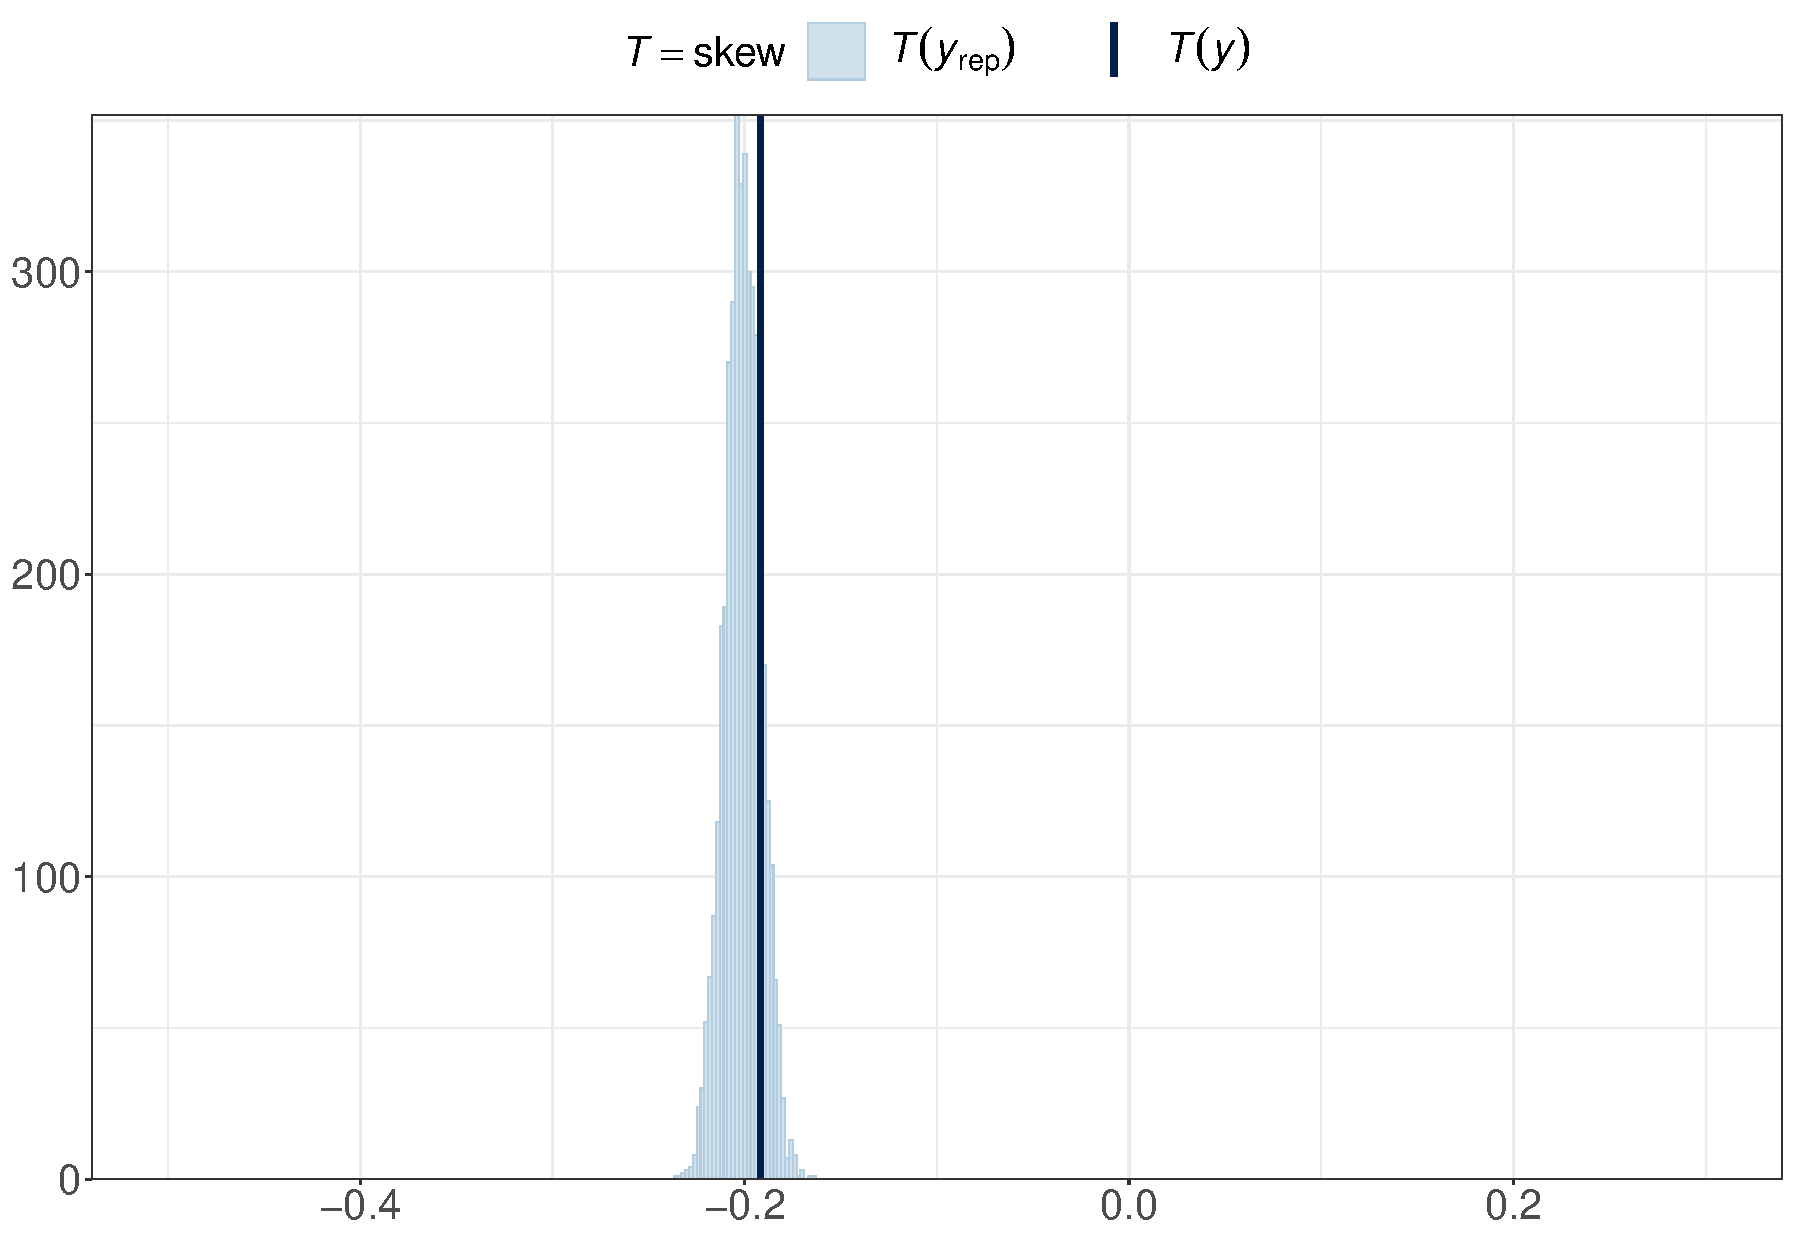
\includegraphics[width=\linewidth]{Images/skew_GSRand_scale.pdf}
			\caption{Skew check of Model 2}
		\end{subfigure}
		\begin{subfigure}[t]{0.45\textwidth}
			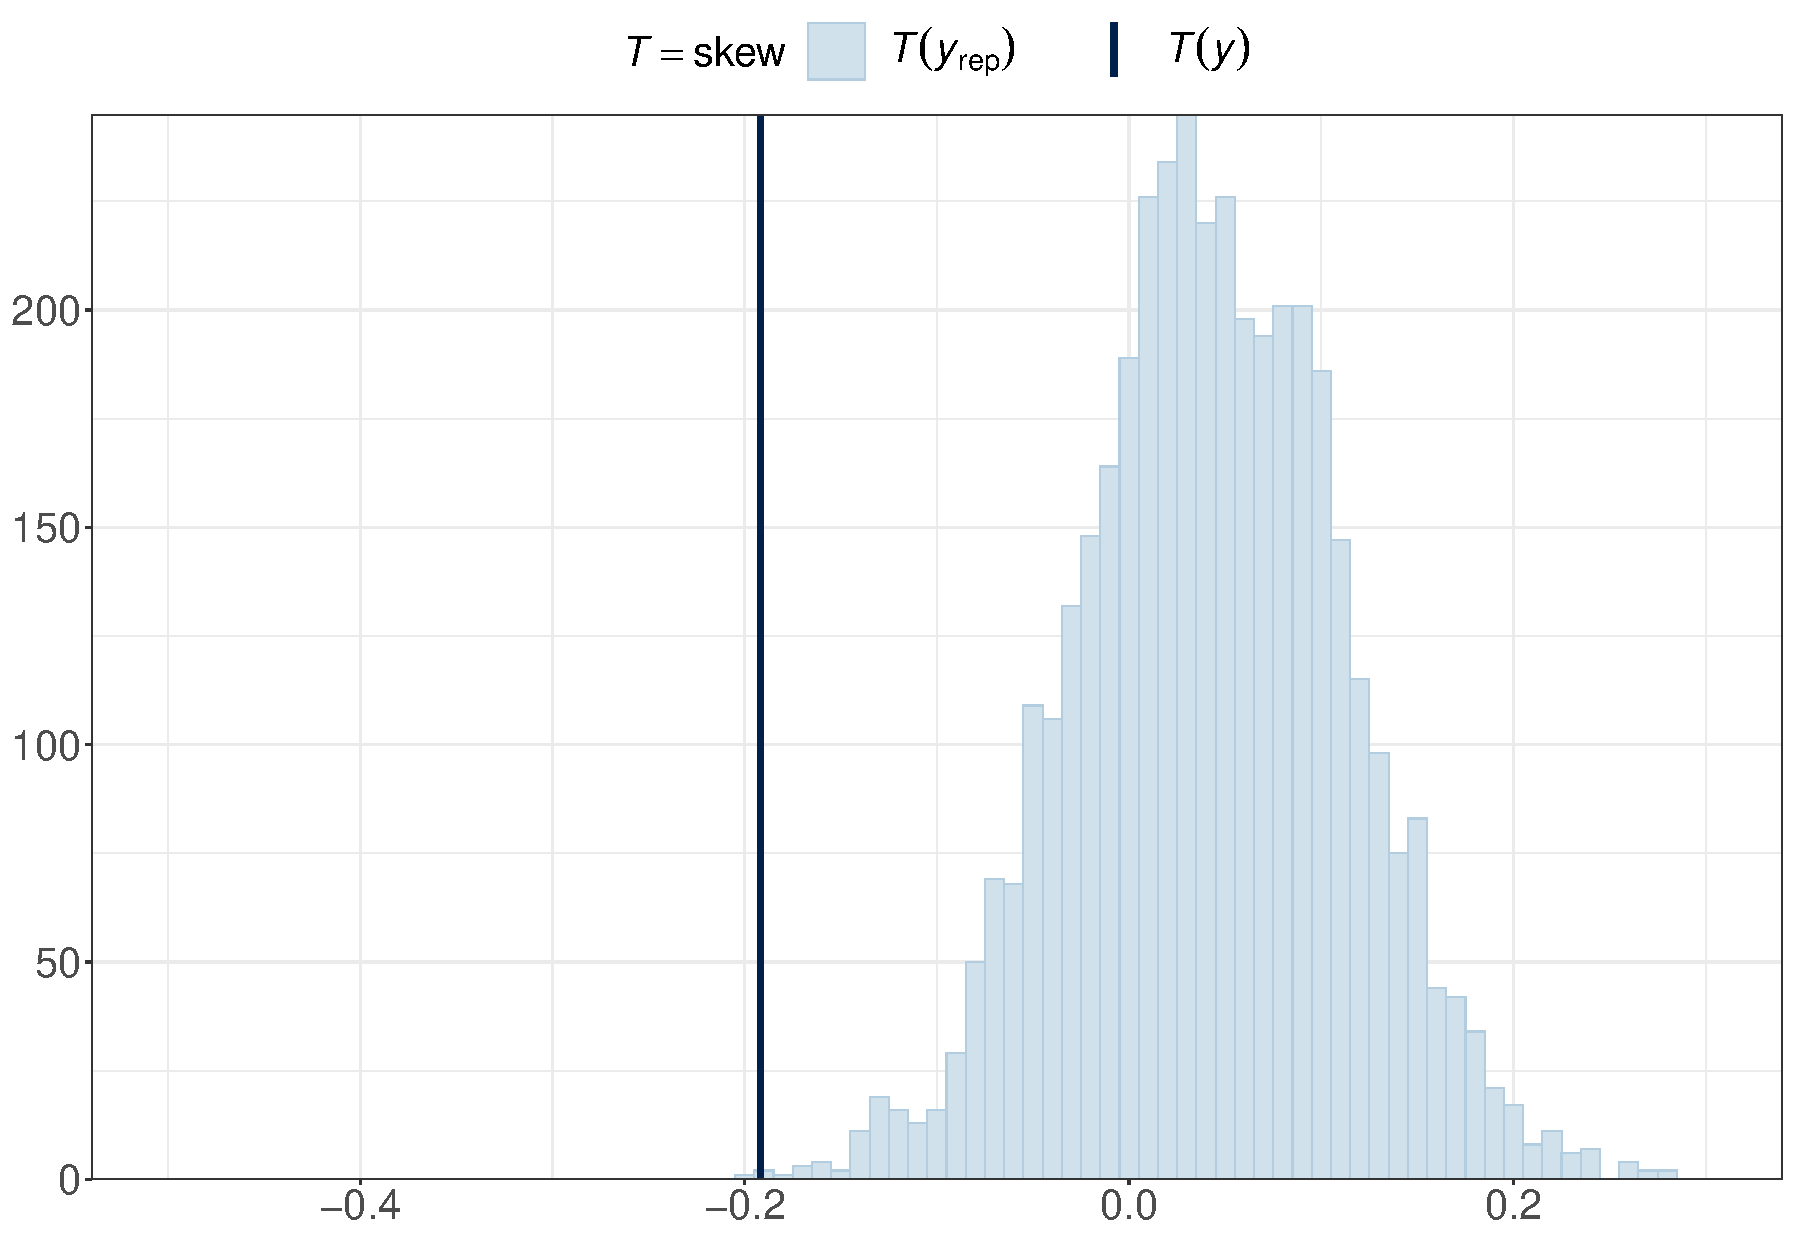
\includegraphics[width=\linewidth]{Images/skew_STRNS_scale.pdf}
			\caption{Skew check of Model 3}
		\end{subfigure}
		\begin{subfigure}[t]{0.45\textwidth}
			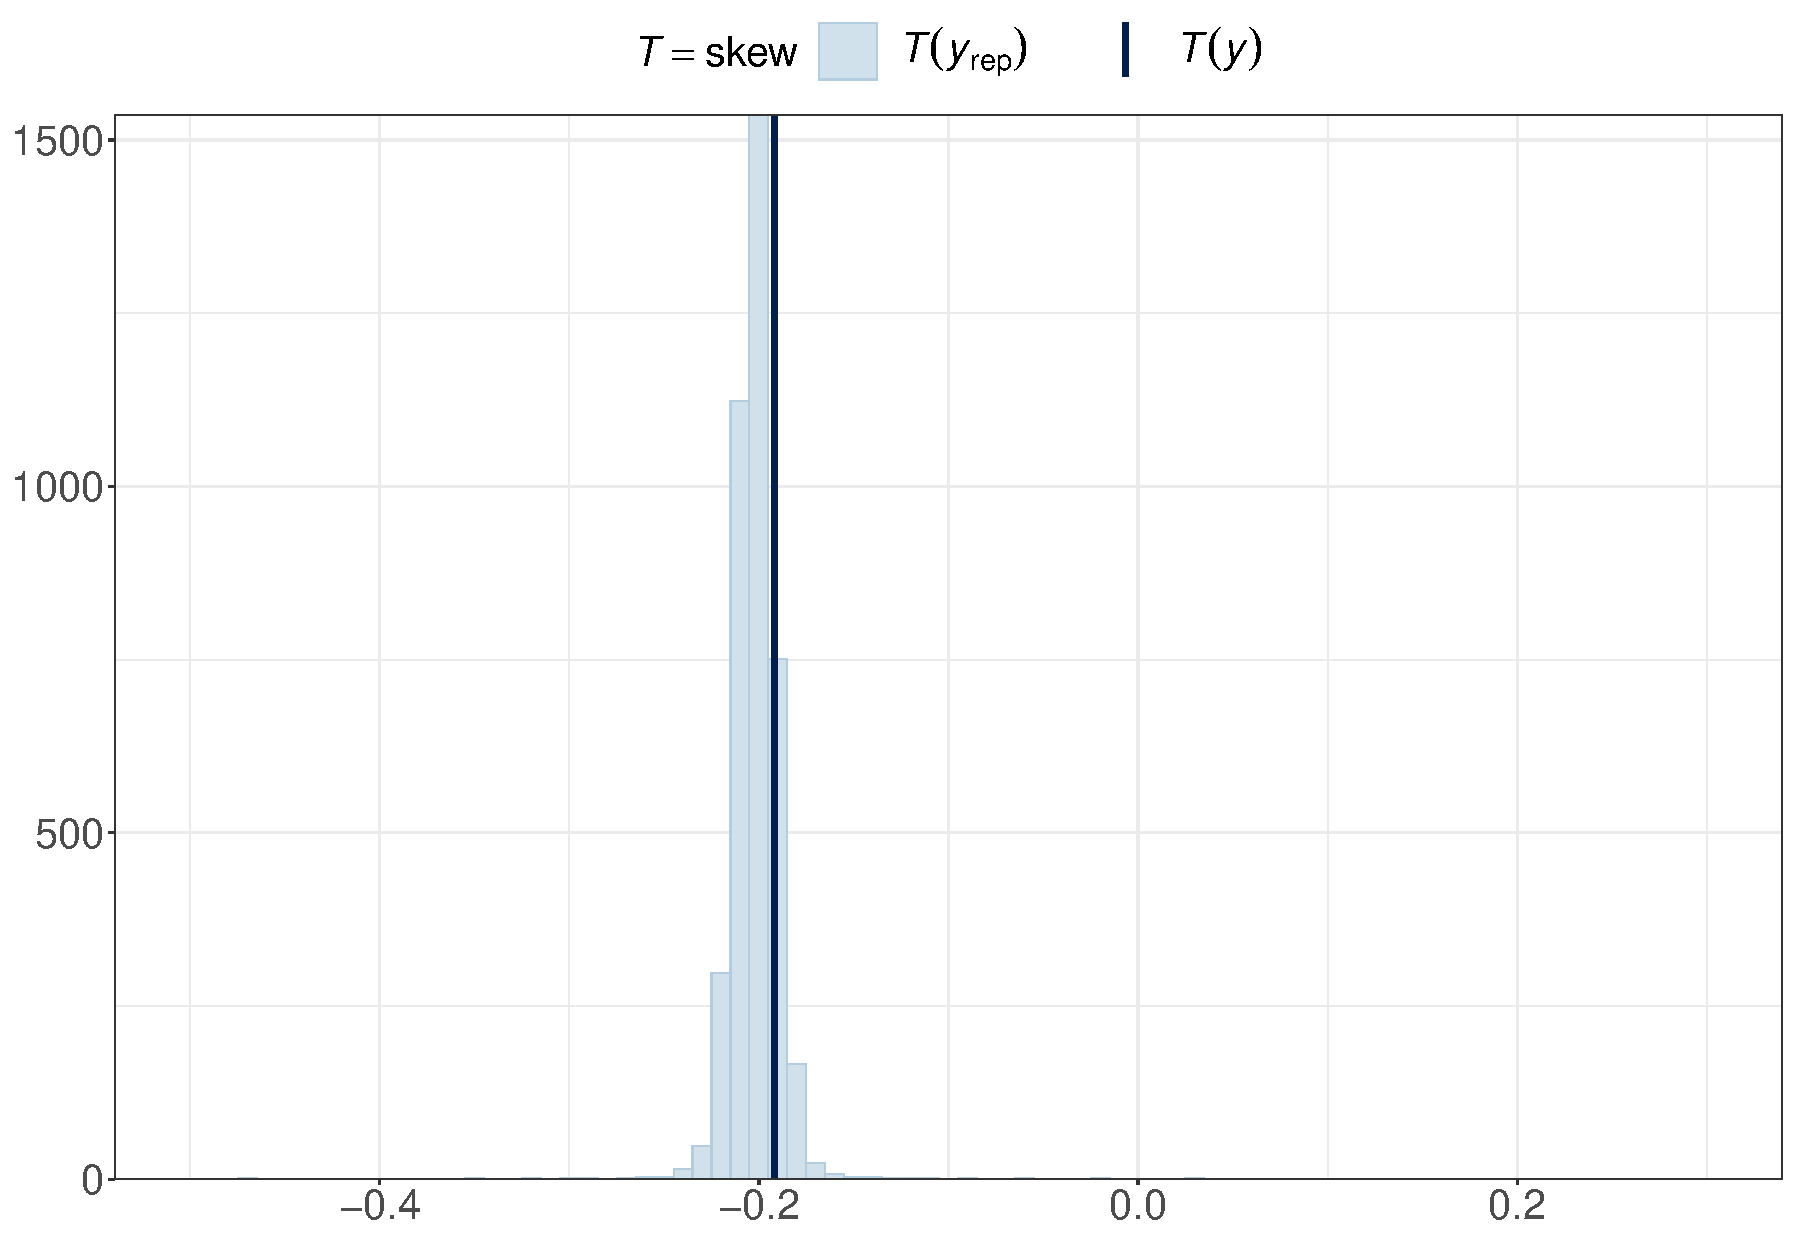
\includegraphics[width=\linewidth]{Images/skew_STRand_scale.pdf}
			\caption{Skew check of Model 4}
		\end{subfigure}
		\caption{Histograms of skewness for 4000 draws (blue) from the posterior predictive distribution comparing to the observed data (black).}\label{fig:skewcheck}
	\end{figure}
	
	
	LOO CV predictive cumulative density plots are used to visualise the performance of the models. The model is well calibrated when the plots are asymptotically uniform (for continuous data) \parencite{gabry2019Visualization, Gelman2013Bayesian}. Figure \ref{fig:pitloo} compares the density of the computed leave one out probability integral transformation (LOO PIT) (the thick dark curve) versus 100 simulated data sets from a standard uniform distribution (the thin light curves). Model 1 and 3 are obviously miscalibrated. Overall, the fit for Model 2 is good but the frown shape of the curve indicates a little miscalibration in comparison to Model 4. This implies that the model is either misspecified or too flexible. A flexible model has a good capability in predicting out-of-sample data. Among all four models Model 4 demonstrates the best fit.
	
	\begin{figure}[!htp]
		\centering
		\begin{subfigure}[t]{0.45\textwidth}
			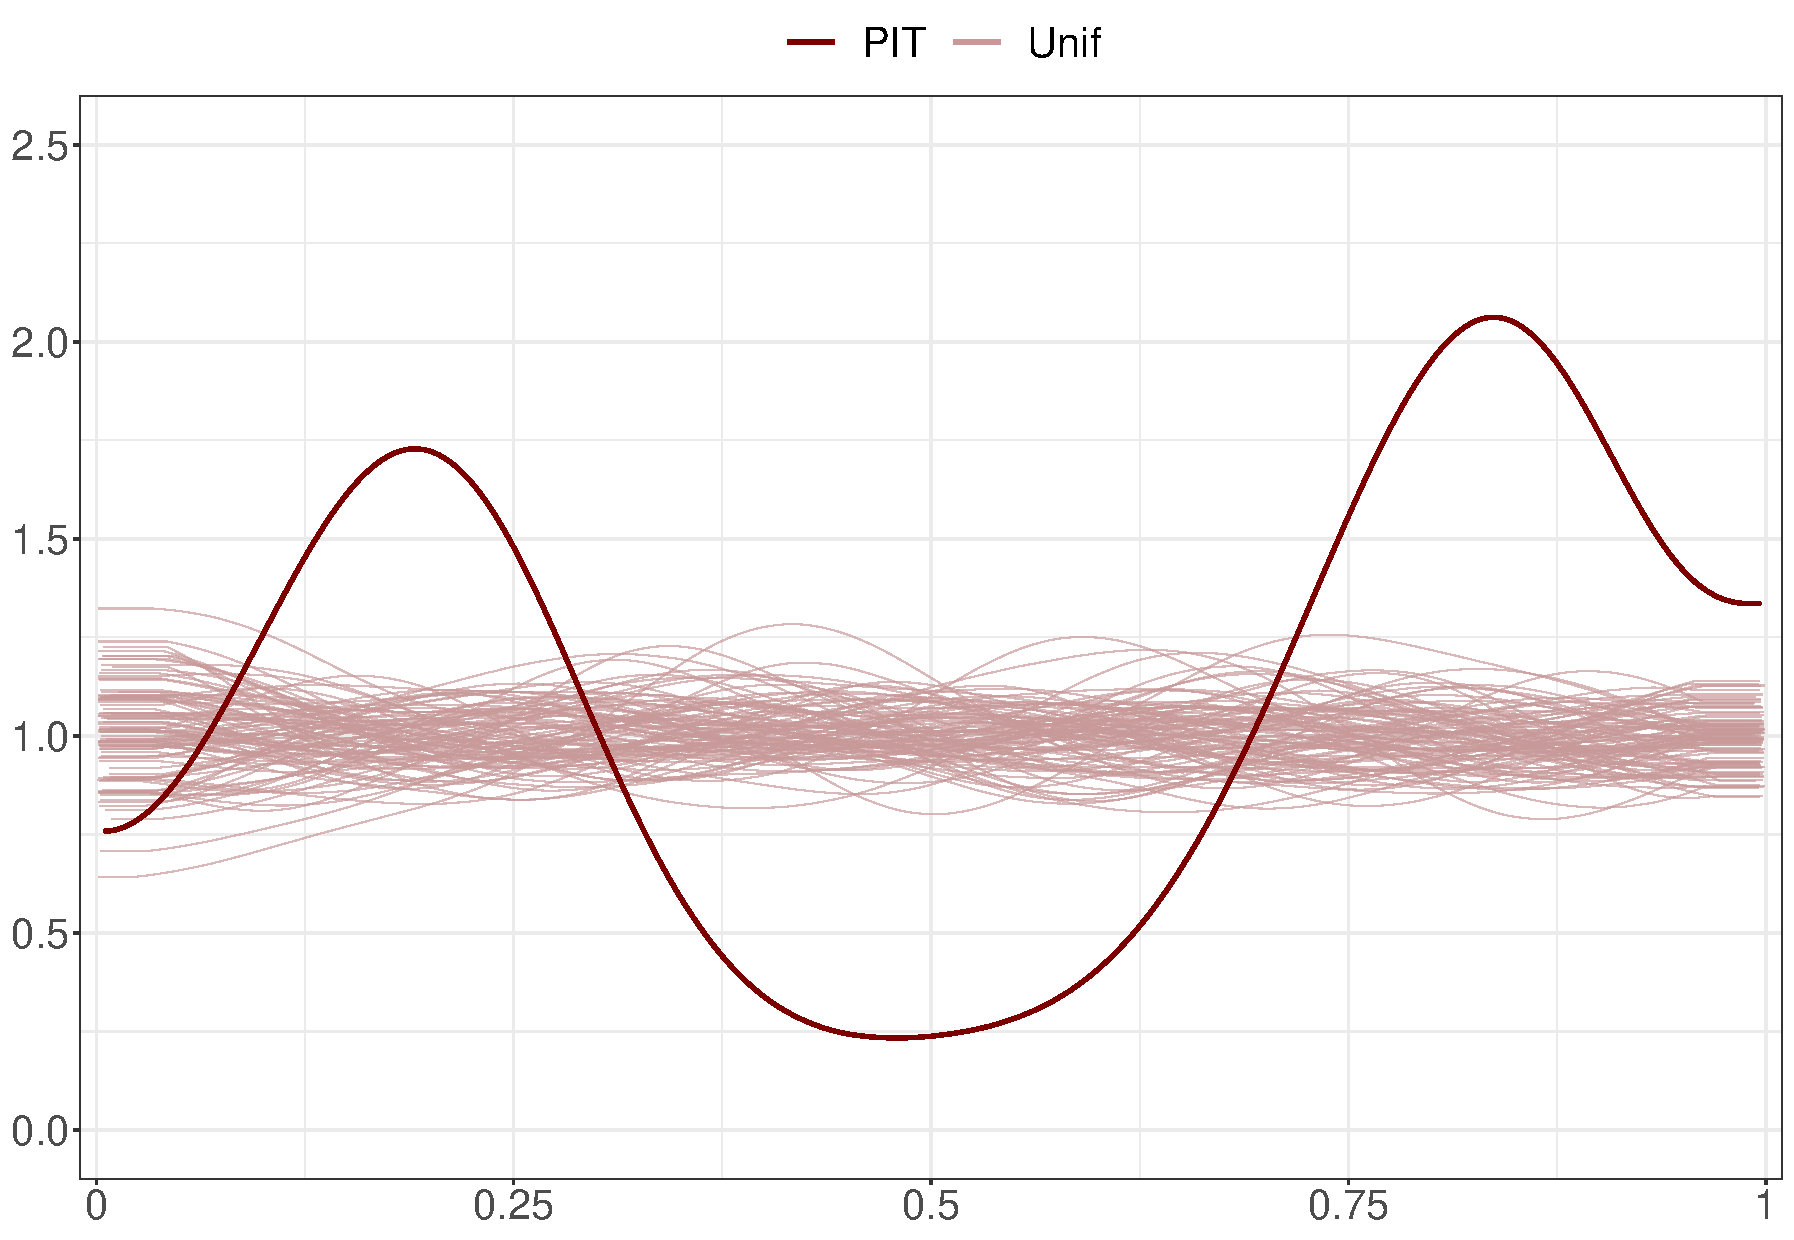
\includegraphics[width=\linewidth]{Images/pit_GSRNS_scale.pdf}
			\caption{LOO PIT diagnosis of Model 1}
		\end{subfigure}
		\begin{subfigure}[t]{0.45\textwidth}
			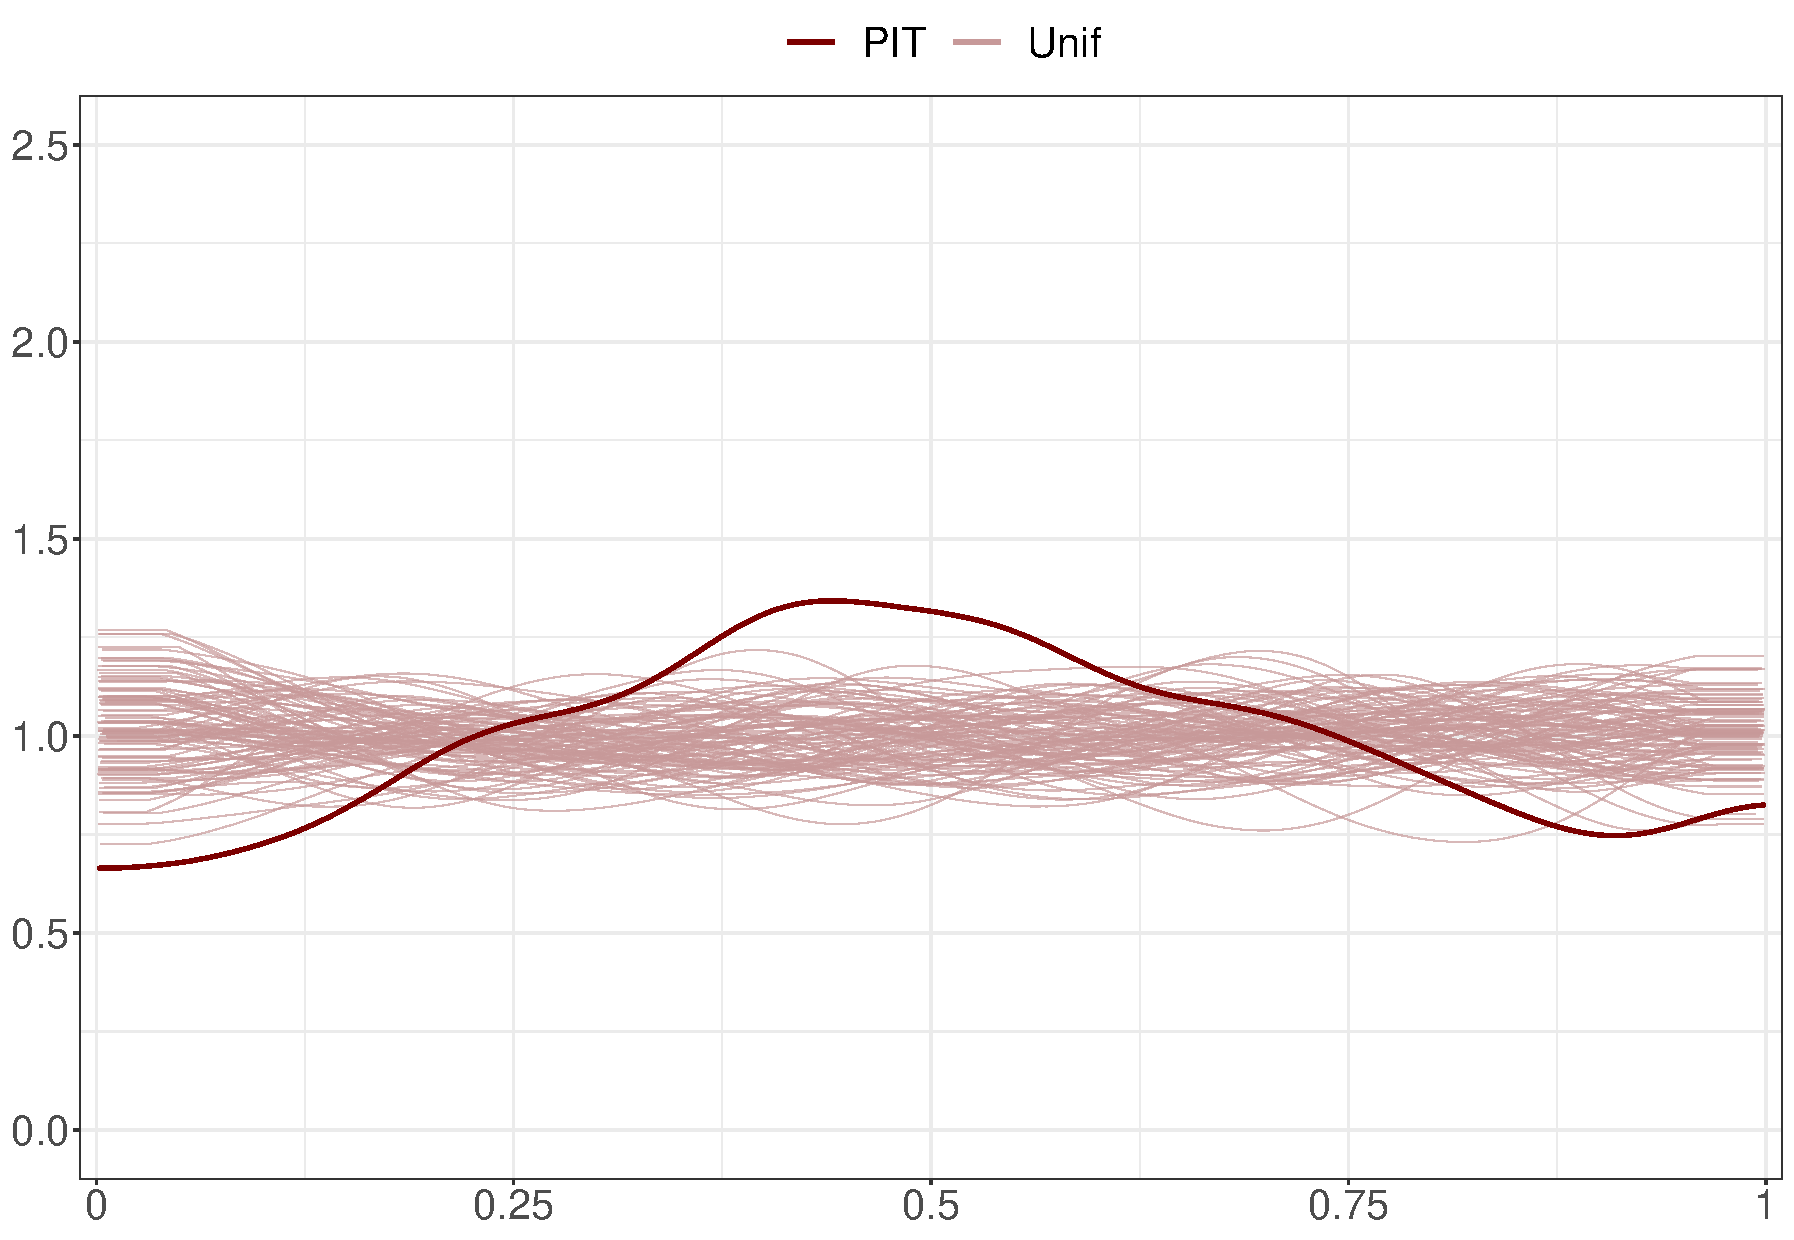
\includegraphics[width=\linewidth]{Images/pit_GSRand_scale.pdf}
			\caption{LOO PIT diagnosis of Model 2}
		\end{subfigure}
		\begin{subfigure}[t]{0.45\textwidth}
			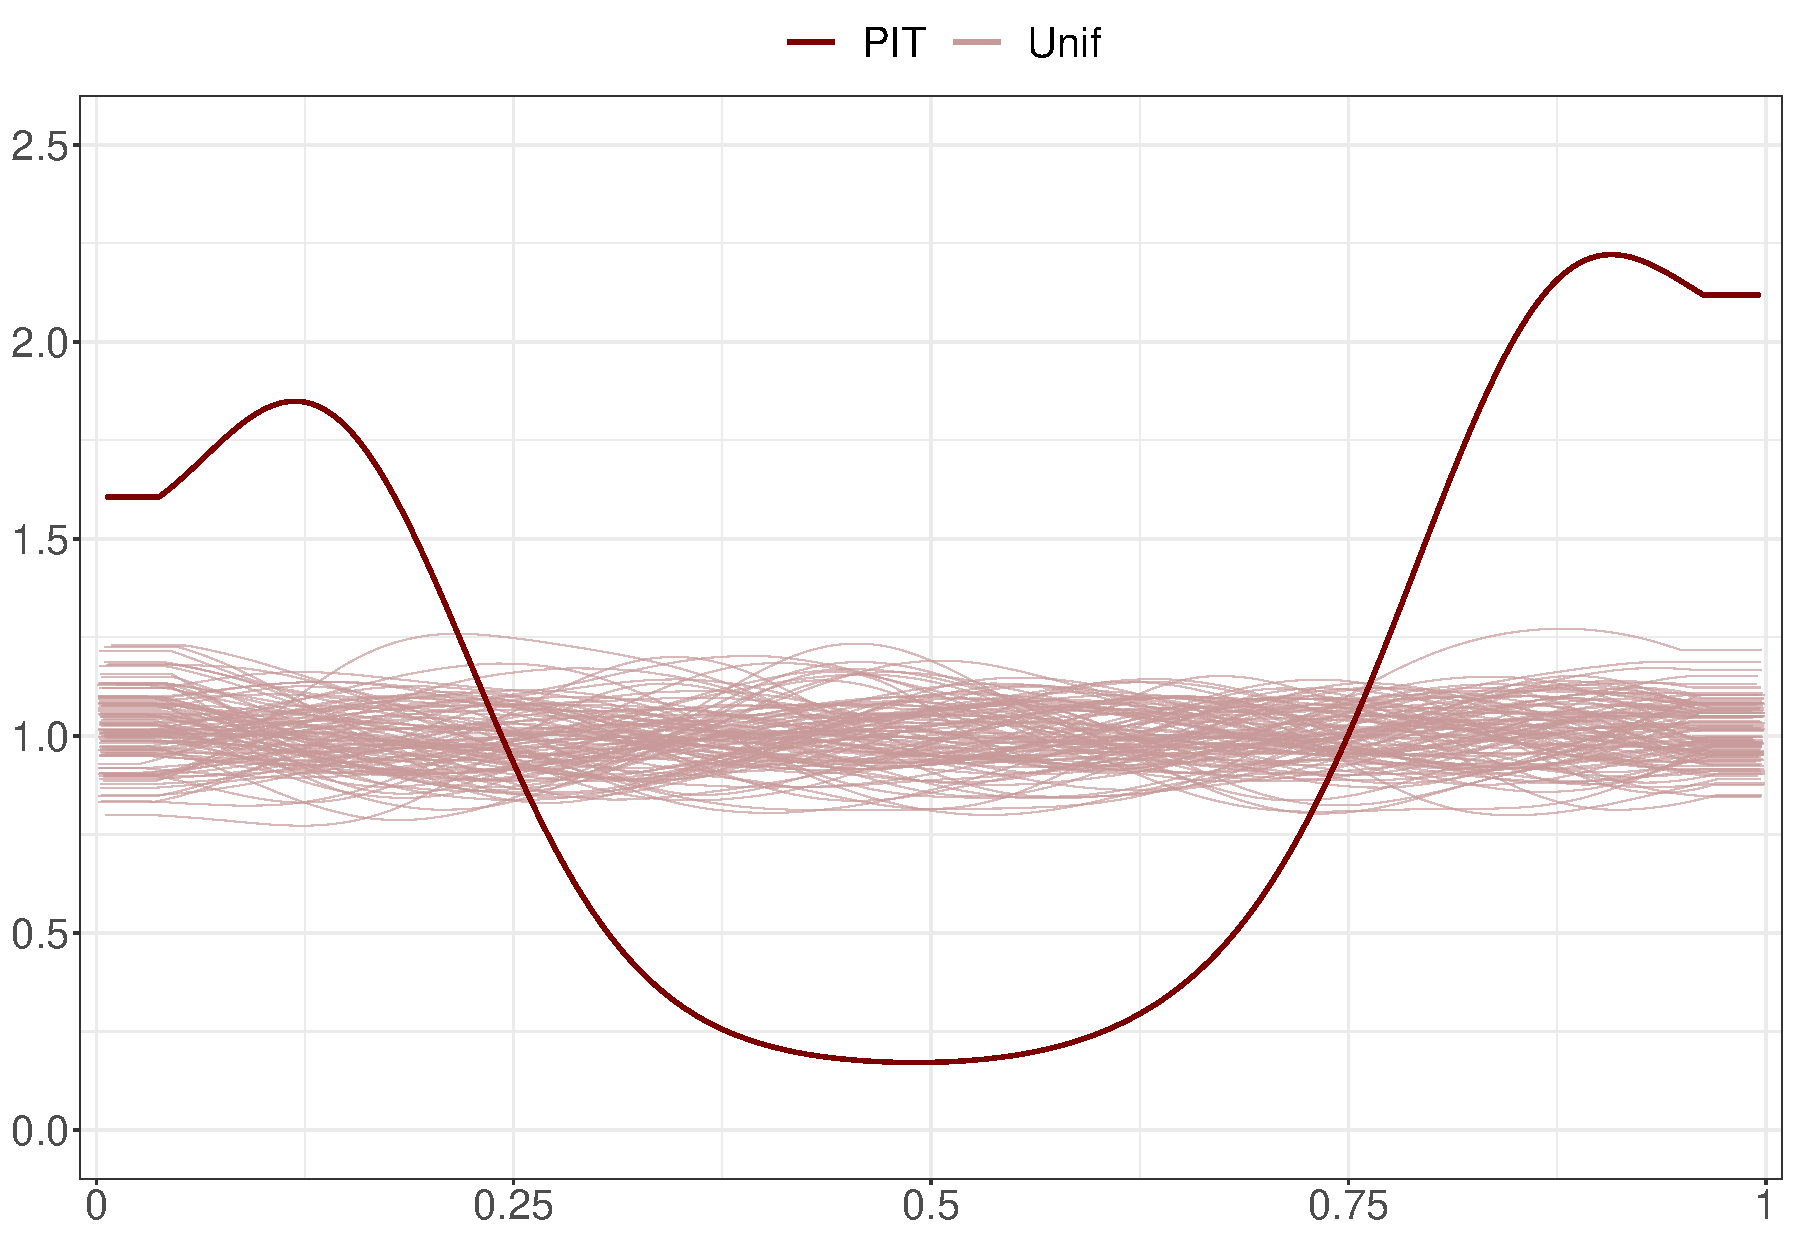
\includegraphics[width=\linewidth]{Images/pit_STRNS_scale.pdf}
			\caption{LOO PIT diagnosis of Model 3}
		\end{subfigure}
		\begin{subfigure}[t]{0.45\textwidth}
			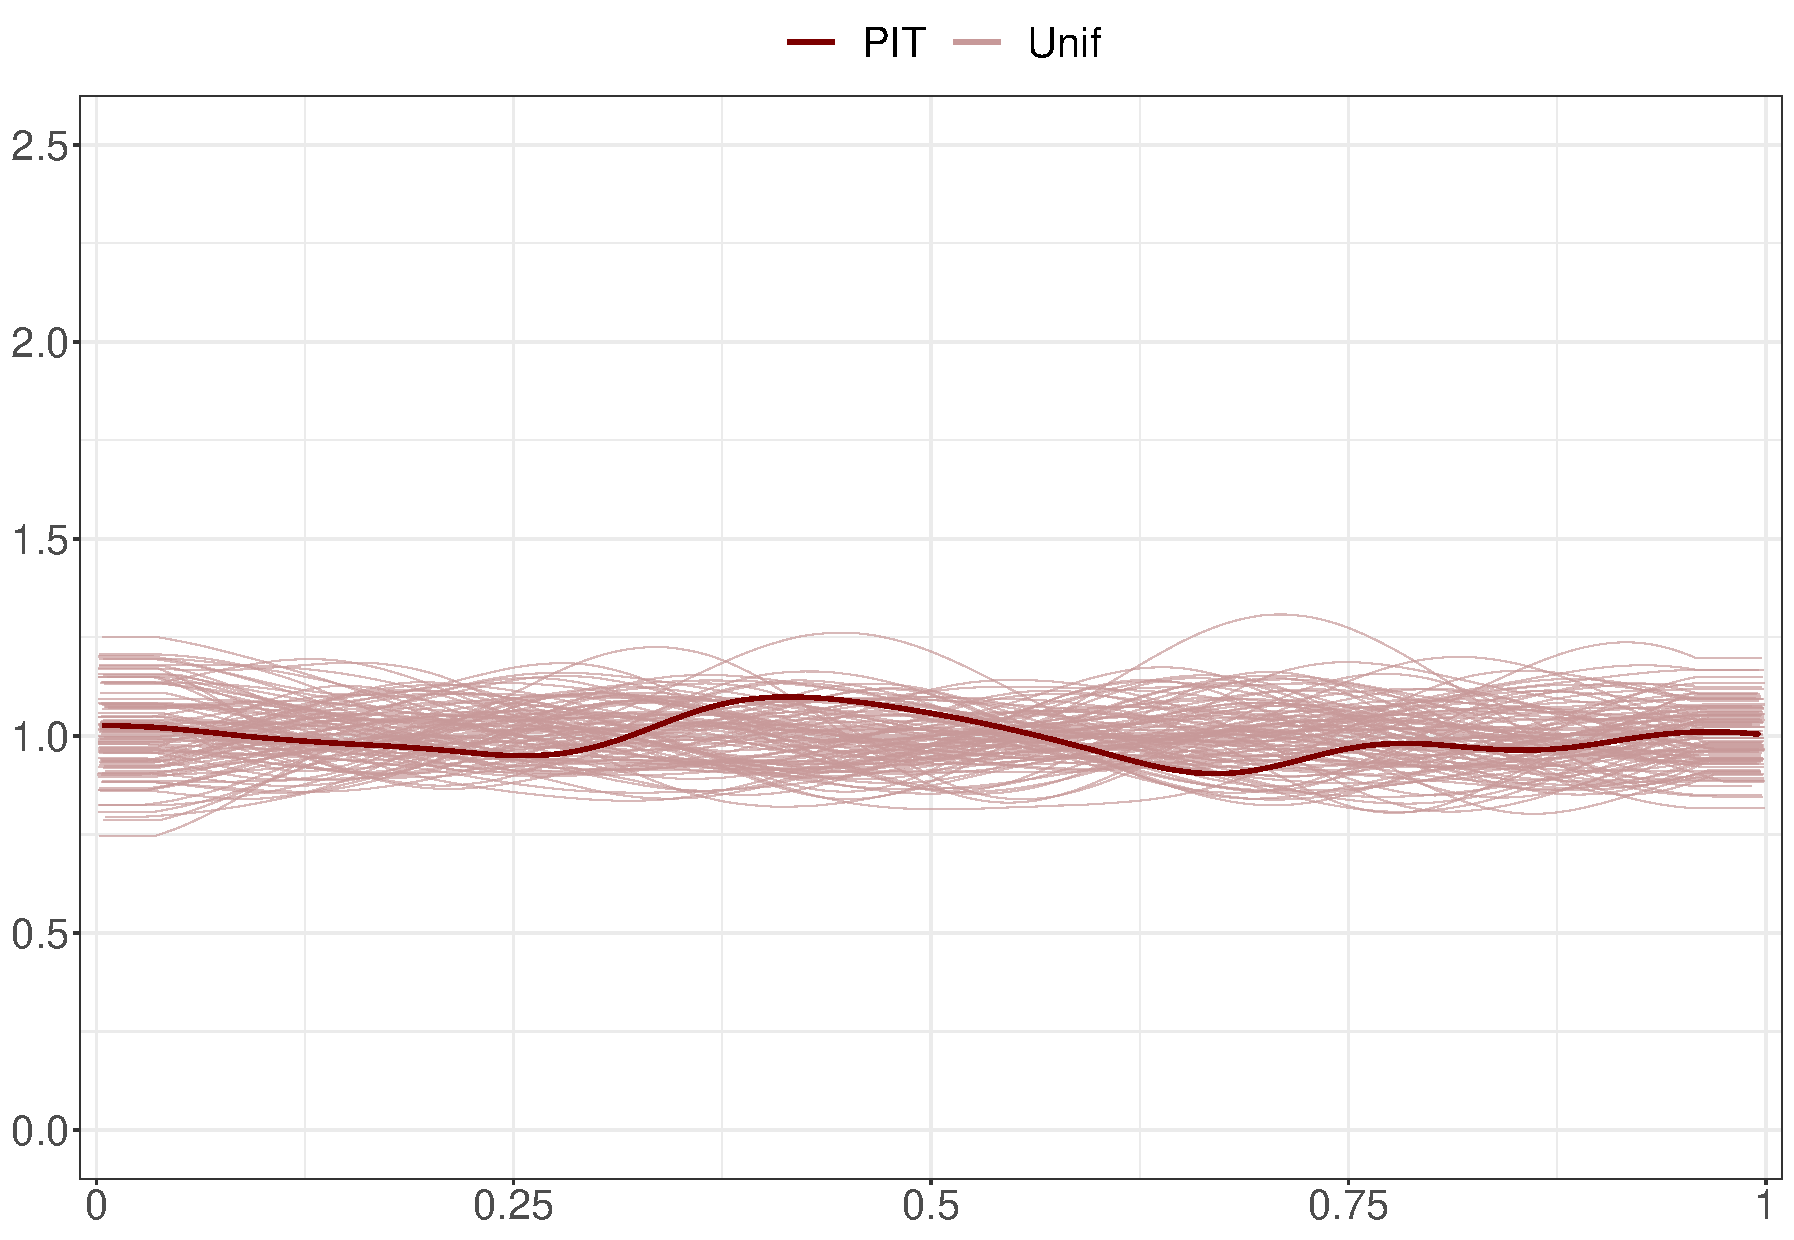
\includegraphics[width=\linewidth]{Images/pit_STRand_scale.pdf}
			\caption{LOO PIT diagnosis of Model 4}
		\end{subfigure}
		\caption{LOO PIT plots of the four models. The thick dark line is the density of the LOO PIT for each candidate model, and the thin lines are simulated data from a standard uniform distribution. }\label{fig:pitloo}
	\end{figure}
	
	
	Pareto $\hat{k}$ diagnostic value is also important, as shown in Table \ref{tb:Pareto}. Model 1 has too many large $\hat{k}$ values, which indicates that the model is either misspecified or too flexible. A similar interpretation can be made for Model 3 where a few ``bad'' values can be observed. These results should not be interpreted solely based on the computed $\hat{k}$ values in Table \ref{tb:Pareto}, but we need to take into account the values of LOO PIT and the effective number of parameters \ploo\ in Table \ref{tb:LOOR}. The \ploo\ is calculated by subtracting the \elpd\ from the full $\log$ posterior predictive density. Figure \ref{fig:ppcheck} shows that models 1 and 3 are misspecified. The LOO PIT plots (Figure \ref{fig:pitloo}) also confirm that these two models are misspecified, even though there are no ``very bad'' $\hat{k}$ values. In the case where high Pareto $\hat{k}$ values are observed but the model fit is good, one can conclude that the model is both misspecified and flexible. In this scenario, a $K$-fold CV is recommended instead of LOO CV for some $K \geq 5$. 
	
	For Model 2, there are six ``bad'' and ``very bad'' $\hat{k}$ values, which might be due to highly influential points or outliers. These large $\hat{k}$ values also indicate the potential misspecification of the Gaussian likelihood. Therefore, instead of using Gaussian distribution, Model 4 uses the Student-$t$ distribution. The selection of the Student-$t$ distribution resulted in improvement in all $\hat{k}$ values, as these are estimated to be less than the threshold value of $0.70$. Then the \elpd\ and Bayesian $R^2$ are valid. 
	
	\begin{table}[!htp]
		\centering
		\resizebox{\textwidth}{!}{
			\begin{tabular}{ l *{12}{c} } \toprule 
				& \multicolumn{3}{c}{Model 1}   & \multicolumn{3}{c}{Model 2} & \multicolumn{3}{c}{Model 3}   & \multicolumn{3}{c}{Model 4} \\
				&  Count & Per & M.Eff  &  Count & Per & M.Eff  &  Count & Per & M.Eff  &  Count & Per & M.Eff   \\ \midrule
				(-Inf, 0.5] (good)  &  28    &  1.7\%   & 457 &  1585  & 94.7\%  & 432     &1474 & 88.1\%& 494 & 1672 & 99.9\% & 868 \\   
				(0.5, 0.7] (ok)      &  372  &  22.2\% & 112 &     83  & 5.0\% &  103  & 176  & 10.5\% & 254 &   2  & 0.1\% & 1733    \\
				(0.7, 1] (bad)       &  1138&  68.0\% & 18   &     4   & 0.2\%  & 70    &  24   &  1.4\%  & 170 &  0    &  0.0\%& ---  \\
				(1, Inf) (very bad)&  136  &  8.1\%   & 8     &     2 &  0.1\%  & 4  &  0    &     0\%   & ---   &  0   & 0\%     & ---  \\
				\bottomrule
		\end{tabular}}
		\caption{Pareto $\hat{k}$ diagnostic values including count, percentage (Per) and minimal effective sample sizes (M.Eff) for all models.}\label{tb:Pareto}
	\end{table}
	
	
	\subsection{Model evaluation}
		
	We use \textcolor{red}{\elpd, \ploo, LOO information criterion (looic), which is $-2\times$\elpd\ in deviance scale,} and Bayesian $R^2$ to evaluate and compare the performance of different models. In Bayesian analysis, even if there are no high Pareto $\hat{k}$ values, $R^2$ is not indicative if \ploo\ is relatively high compared to the total number of parameters or the number of observations. A high \ploo\ and looic imply weakly predictive capability and a suspicious model misspecification. 
		
	The results for each model are presented in Table \ref{tb:LOOR}. The mean and standard deviation of the posterior distribution, along with the credibility interval (CI) are reported. The equal tail CI at level $\alpha$ is the interval bracketed by the $\alpha/2$ and the $1-\alpha/2$ quantiles of the posterior samples, where $\alpha \in (0,1)$. We chose $\alpha=0.05$, a standard option in frequentist statistics. 	
	
	\begin{table}[!htp]
		\centering
		\resizebox{\textwidth}{!}{\begin{tabular}{ l *{8}{c} } \toprule 
				& \multicolumn{2}{c}{Model 1}   & \multicolumn{2}{c}{Model 2} & \multicolumn{2}{c}{Model 3}   & \multicolumn{2}{c}{Model 4} \\
				\midrule
				&  Estimate & SE &  Estimate & SE &  Estimate & SE &  Estimate & SE    \\ 
				\elpd &  -7236.2  & 13.4 & -4945.2 & 134.8&-7848.4 & 17.1 & -4734.3 & 38.3 \\   
				\ploo  & 1487.1     & 11.7 & 341.8 & 41.3 &241.2  & 6.8 & 516.1 & 10.5 \\
				looic     &  14472.5  & 26.7 & 9890.4 & 269.6 &  15696.8 & 34.3 & 9468.7 & 76.7\\		
				\midrule
				&  Median & CI &   Median & CI &   Median & CI &   Median & CI   \\ 
				Bayesian $R^2$   &  0.842   & 0.563$\sim$0.965 &  0.974  & 0.972$\sim$0.977 & 0.190 & 0.135$\sim$0.251 & 0.987 & 0.989$\sim$0.991 \\
				\bottomrule
		\end{tabular}}
		\caption{LOO CV estimates with standard errors and medians of Bayesian $R^2$ with credibility intervals.}\label{tb:LOOR}
	\end{table}
		
	The $R^2$ is valid only when the model is not misspecified. In the results, Model 1 is better than Model 3 in terms of the higher $R^2$ value. But these two models are all misspecified according to high Pareto $\hat{k}$ values and large \ploo\ values. Therefore, $R^2$ is not indicative for neither Model 1 and Model 3. The focus should be on Models 2 and 4. Apparently, Model 4 with Student-$t$ distribution is better than Model 2 with Gaussian distribution in terms of smaller looic and higher $R^2$ value. The bad Pareto $\hat{k}$ values in Model 2 are eliminated by fitting Model 4. 
	
	
	
	\section{Results}\label{sec:results}
	
	In the previous section, through model selection and evaluation process, we found that Model 4 fits the data best. It proves the capability of spatially correlated random parameters in capturing the spatial variation. With the Bayesian inference of all parameters and model \eqref{eq:prediction}, we are able to obtain a smooth map showing the optimal level of the treatment across a grid made by rows and columns covering the whole field, and hence the estimated yield map. 
		
	
	\subsection{Model assessment}
	Table \ref{tb:resultModel4} presents the summary statistics of the posterior distribution of all parameters from Model 4. It should be noted that the means and the medians for all parameters are very close or identical which indicates robust results. Another feature is that the magnitude of the values of $\hat{b}_2$ and $\hat{\sigma}_2$ are very small. It indicates a week influence of the quadratic term of the regression. The pattern of coefficients magnitude is well illustrated in Figure \ref{fig:betasprd}.
	
	\begin{table}[!htp]\centering
		\begin{tabular}{ l *{5}{c}} \toprule
			\multirow{2}{*}[-2pt]{Parameter}  &  \multirow{2}{*}[-2pt]{Mean}   & \multirow{2}{*}[-2pt]{SD}  &   \multicolumn{3}{c}{Credibility interval}  \\  \cmidrule{4-6} 
			&     &    &    2.5\%   &       Median  &      97.5\% \\ \midrule 
			$\hat{b}_0$   &  80.7214 &  3.0461 & 74.9528 & 80.7003& 86.7650    \\
			$\hat{b}_1$   &  0.0126 &   0.0091 &  -0.0049 &   0.0127 &  0.0303 \\
			$\hat{b}_2(\times 10^{4})$   & 1.9850 & 1.0945 & -1.3057 & 1.9776   &4.1425  \\
			$\hat{\sigma}_0$&  9.1322 & 0.3902  & 8.4027  & 9.1271  & 9.9447   \\
			$\hat{\sigma}_1$&  0.0173  & 0.0071  & 0.0034  & 0.0174  &  0.0314   \\
			$\hat{\sigma}_2(\times 10^{4})$&   1.7157  & 0.7151  & 0.3935  & 1.6742  & 3.2388   \\		
			$\hat{\sigma}_e$& 2.6399  & 0.1244  & 2.3953  & 2.6398  & 2.8905   \\
			$\hat{\rho}_{12}$& -0.6493 & 0.2467 & -0.9623 & -0.7005 & -0.0115 \\
			$\hat{\rho}_{13}$& 0.5367 & 0.2481 & 0.0193 & 0.5514 & 0.9480   \\
			$\hat{\rho}_{23}$&-0.4282 &  0.3754 & -0.9361 & -0.5033 &  0.4732  \\		
			$\hat{\rho}_c$   & 0.9076 & 0.0115 & 0.8835 & 0.9080 & 0.9287   \\
			$\hat{\rho}_r$   &  0.9274 & 0.0074&  0.9120& 0.9275 & 0.9410  \\
			$\hat{\nu}$ &  4.1321 & 0.5503 & 3.2098 & 4.0861 & 5.3573  \\
			\bottomrule
		\end{tabular}\caption{Summary statistics of the posterior samples from Model 4. Mean, standard deviation (SD), credibility interval and median of posterior samples are reported. }\label{tb:resultModel4}
	\end{table}         
	
	Figure \ref{fig:betasprd} displays the overall coefficients of the fixed and random components on three separate plots, for the intercept $\hat{\bm{\beta}}_0 = \hat{\bm{b}}_0+\tilde{\bm{u}}_0$, the linear term $\hat{\bm{\beta}}_1 = \hat{\bm{b}}_1+\tilde{\bm{u}}_1$ and the quadratic term $\hat{\bm{\beta}}_2 = \hat{\bm{b}}_2+\tilde{\bm{u}}_2$, respectively. The plots cover the whole trial area, as presented in Figure \ref{fig:lasrossayield} and \ref{fig:lasrossatopo}. 
	The contour maps are aligned with the topology of the area. It can be observed that the Hilltop area and small part of the neighbouring areas on the left and right (see Figure \ref{fig:lasrossatopo}) are exhibiting different pattern in comparison to the other three topological regions, for all of the $\hat{\bm{\beta}}$ coefficients. The linear component coefficient for the Hilltop area is the highest, in the range of 0.02 -- 0.08, while for the other three areas is around -0.01. %The latter explains the observed pattern in the contour map.
	The quadratic component coefficient for the Hilltop area is negative, which indicates that an optimal treatment in the area is available. However, in other areas, the coefficients are positive and a linear pattern is sufficient in model fitting. 
	
	% Furthermore, in the Hilltop (middle area) and eastern of West slope (left side) areas, the quadratic term $\bm{\beta}_2$ is negative, which means the optimal treatment level exists. 
	
	\begin{figure}[!htp]
		\centering	
		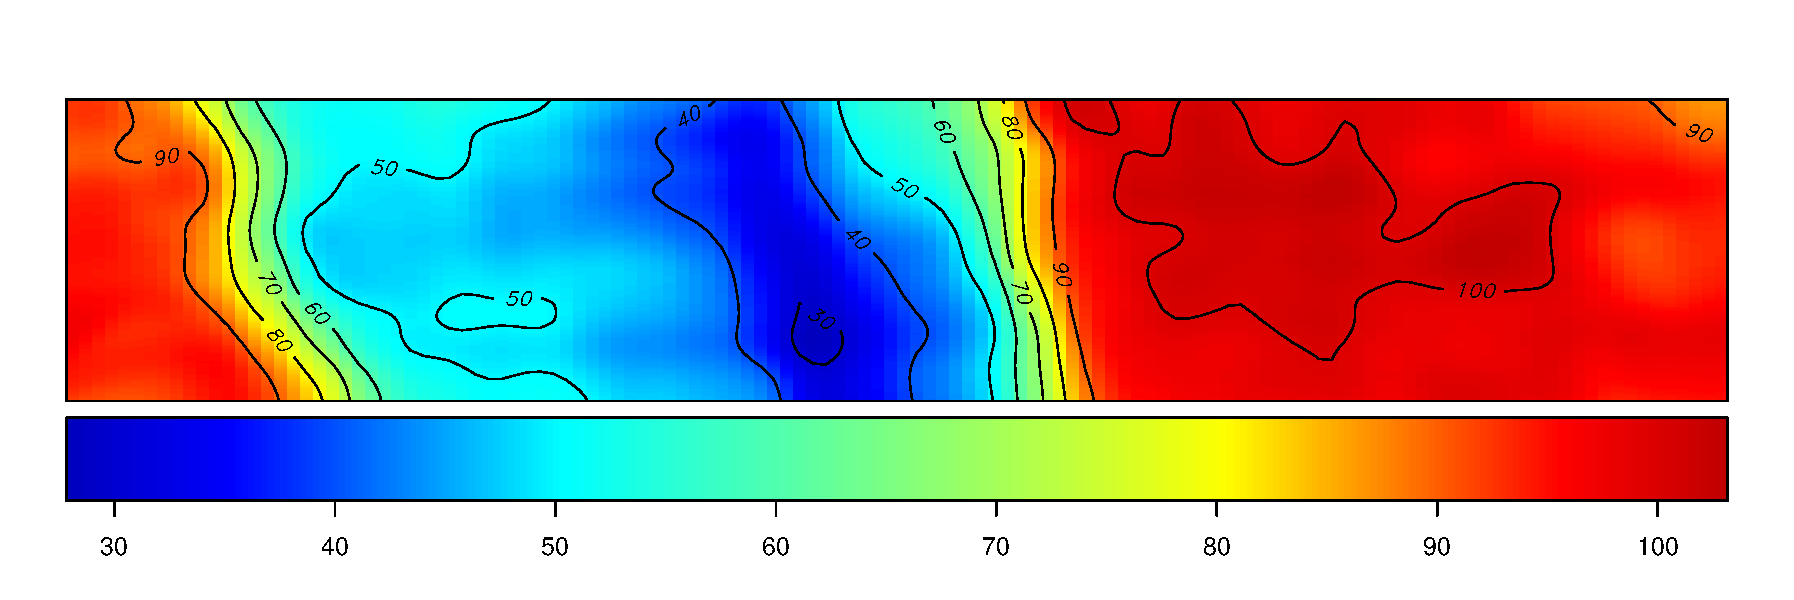
\includegraphics[width=\textwidth, height=6cm]{Images/STRand_b0}
		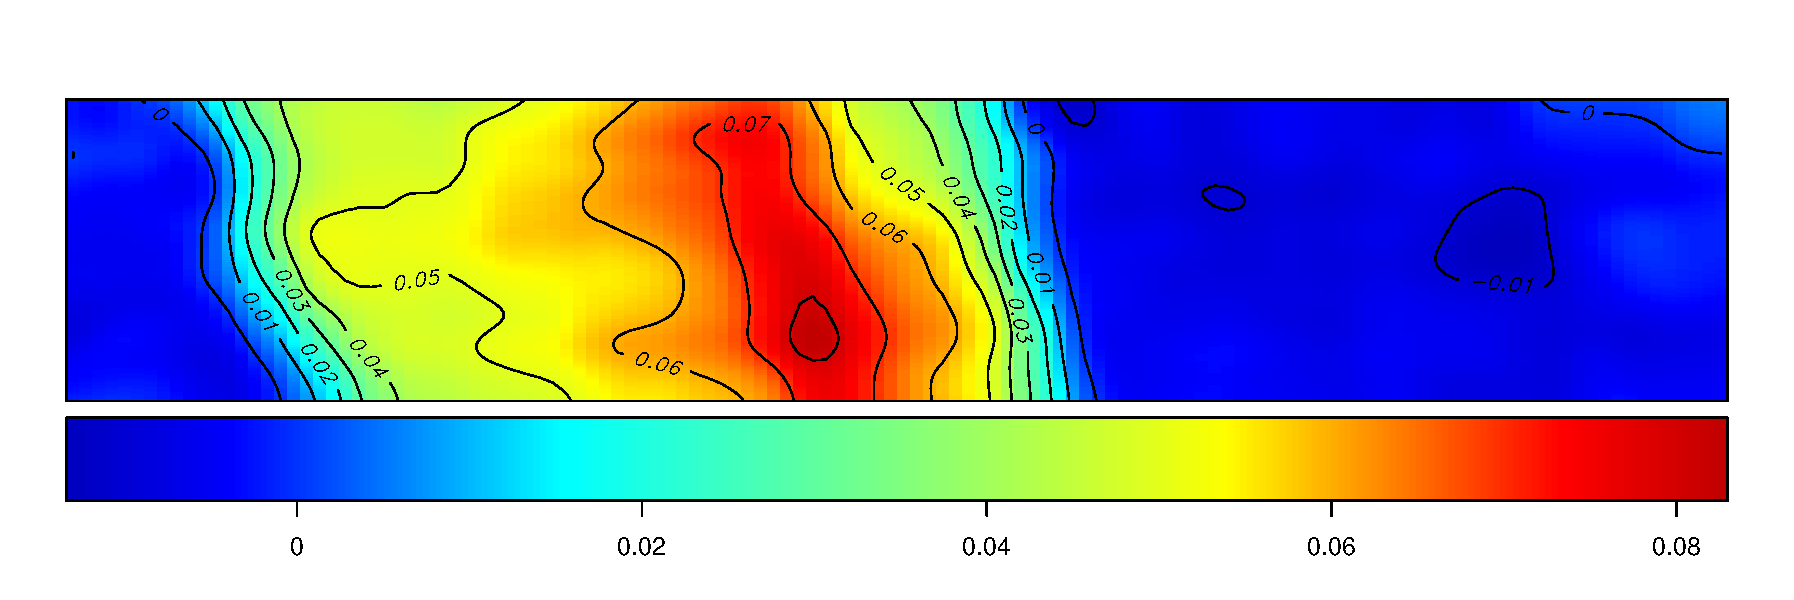
\includegraphics[width=\textwidth, height=6cm]{Images/STRand_b1}
		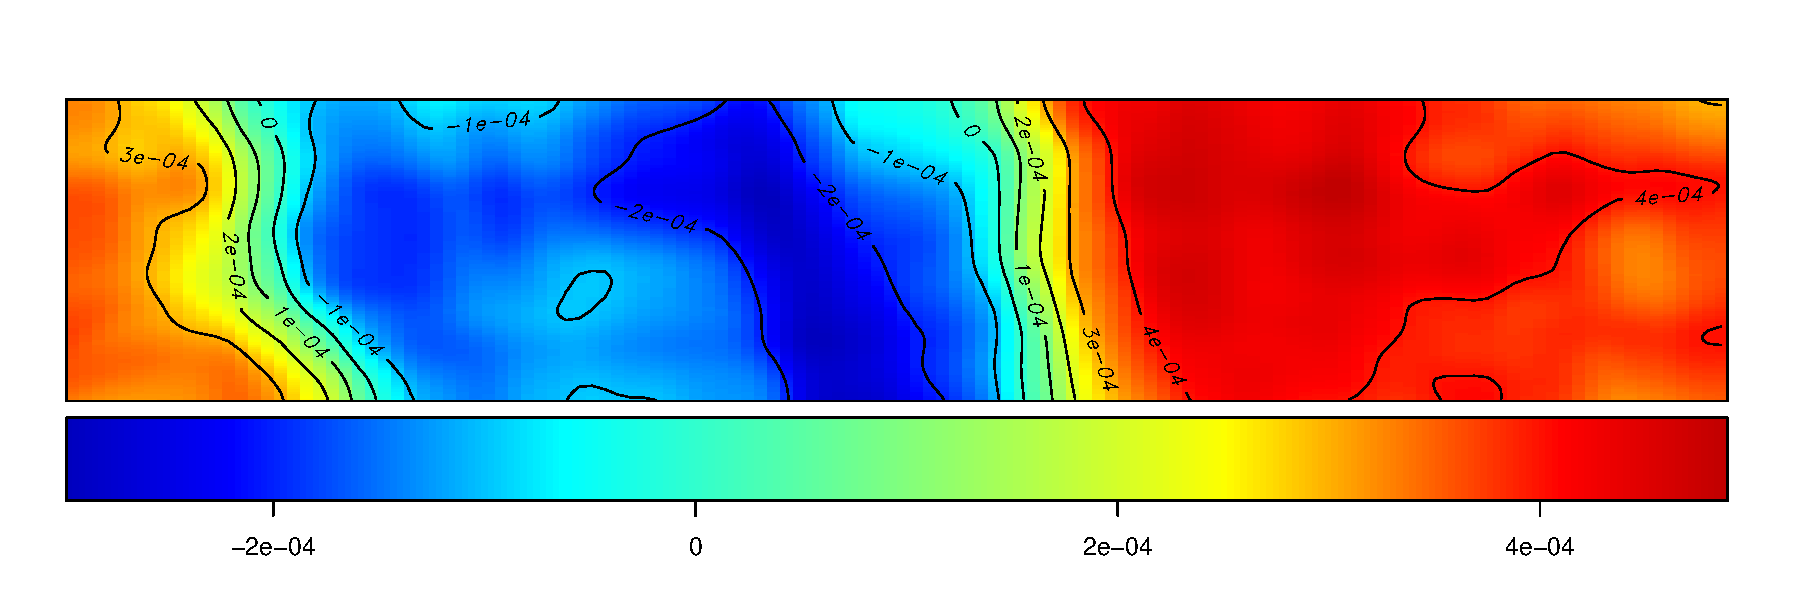
\includegraphics[width=\textwidth, height=6cm]{Images/STRand_b2}
		\caption{Contour plots of spatial-varying coefficients $\hat{\bm{\beta}}_0$ (top), $\hat{\bm{\beta}}_1$ (middle) and $\hat{\bm{\beta}}_2$ (bottom) for Las Rosas data. Negative $\hat{\bm{\beta}}_2$ is available in the Hilltop region, where optimal treatments exist. For other regions, linear response is sufficient. }\label{fig:betasprd}
	\end{figure}
	
	The result is consistent with the discovery by \textcite{Rakshit2020Novel} that the quadratic pattern is strong in Hilltop region but weak in other regions. Even though a quadratic pattern is identified in the East slope and Low East, the adjusted-$p$ values indicate non-significant for these areas. 
	
	\subsection{Yield prediction}
	
%	The results from the previous section allow us to predict yield for any given location with any nitrogen rate. We use the medium nitrogen rate 75.4 kg/ha, as suggested by \textcite{Rakshit2020Novel}, in order to compare the predicted yield across the entire field from both approaches later. After calculating the median yield for each grid, as described above, we obtained the yield map shown in Figure \ref{fig:yieldprd}.	
%	
%	\begin{figure}[!htp]
%		\centering	
%		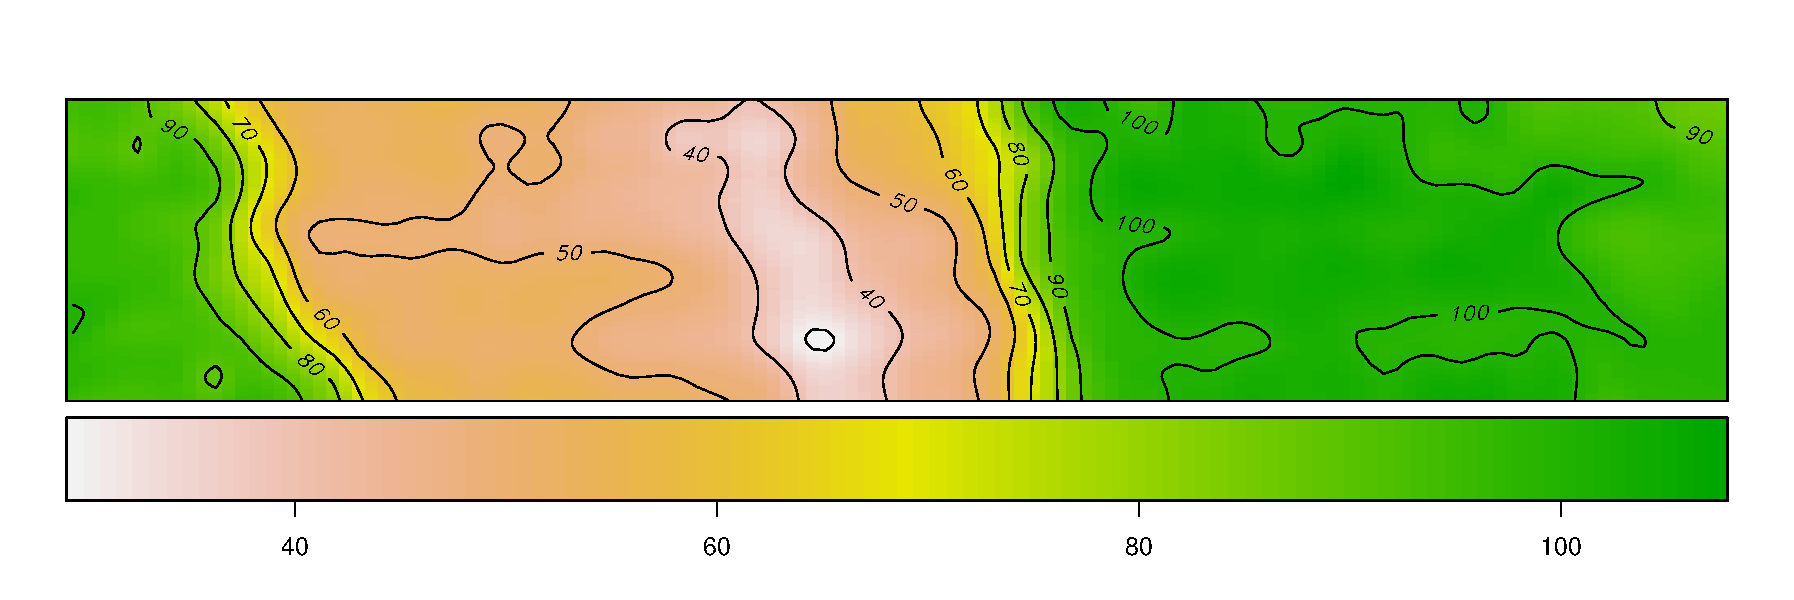
\includegraphics[width=\textwidth]{Images/STRand_prd}
%		\caption{Predicted yield with medium nitrogen rate of 75.4 kg/ha across the field.}\label{fig:yieldprd}
%	\end{figure}
		
	With the assumption that yield is quadratic response of nitrogen rate, hence, optimal nitrogen rate for each grid is available from the model. However, if the optimum rate exceeds the maximum, the maximum is chose. Statistically, $\hat{N}_i = \min\{ \tilde{N}_i, N_{\mbox{max}}\}$ for $i=1,\ldots,n$. Figure \ref{fig:optN} depicts the map of optimal treatment and estimated yield with the optimal treatment on the field. % Most of the area on the field can be applied the maximal nitrogen rate, except the West slope and Hilltop regions that lower rates should be applied. 
		
	\begin{figure}[!htp]
		\centering	
		\includegraphics[width=\textwidth]{Images/ST_opNitrogen_v2}
		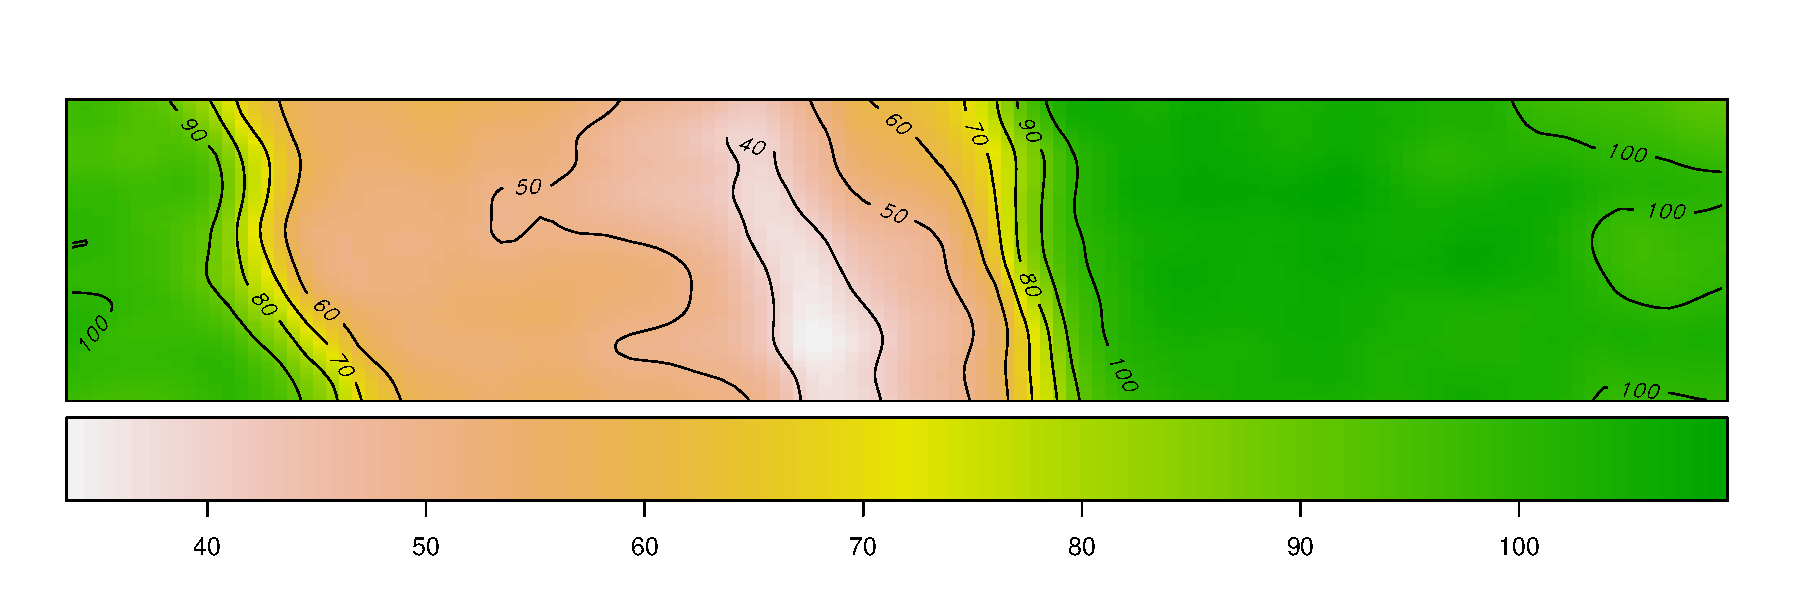
\includegraphics[width=\textwidth]{Images/ST_opYield}
		\caption{Optimal nitrogen rates (top) and estimated yield with the optimal rates (bottom).}\label{fig:optN}
	\end{figure}	
	
% 	After the optimal nitrogen applied on the field, the estimated product is improved comparing to the current yield. Figure \ref{fig:stdiff} illustrates the different yield of the two management strategies. The difference is positive and indicates improvement on yield product. 	
	
% 	\begin{figure}[!htp]
% 		\centering
% 		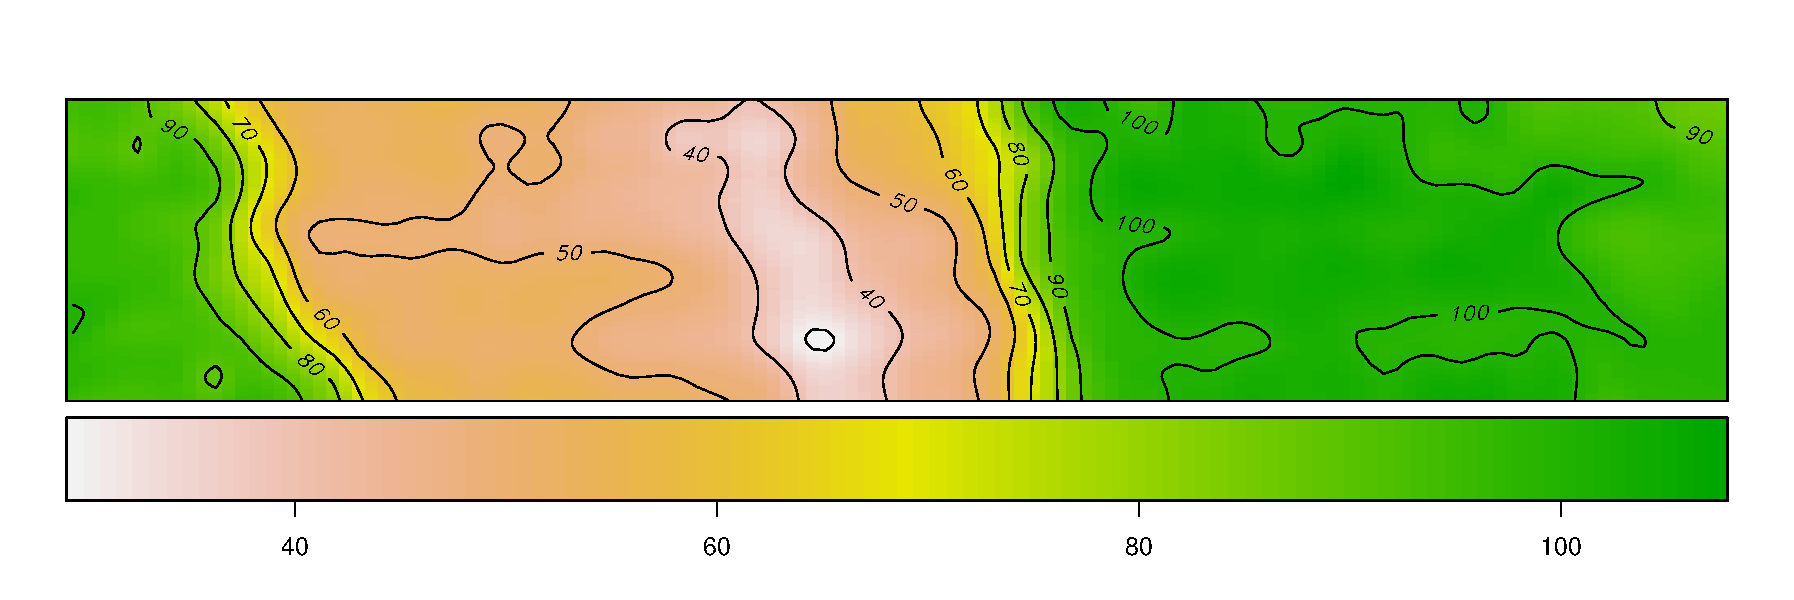
\includegraphics[width=\textwidth]{Images/STRand_prd.pdf}
% 		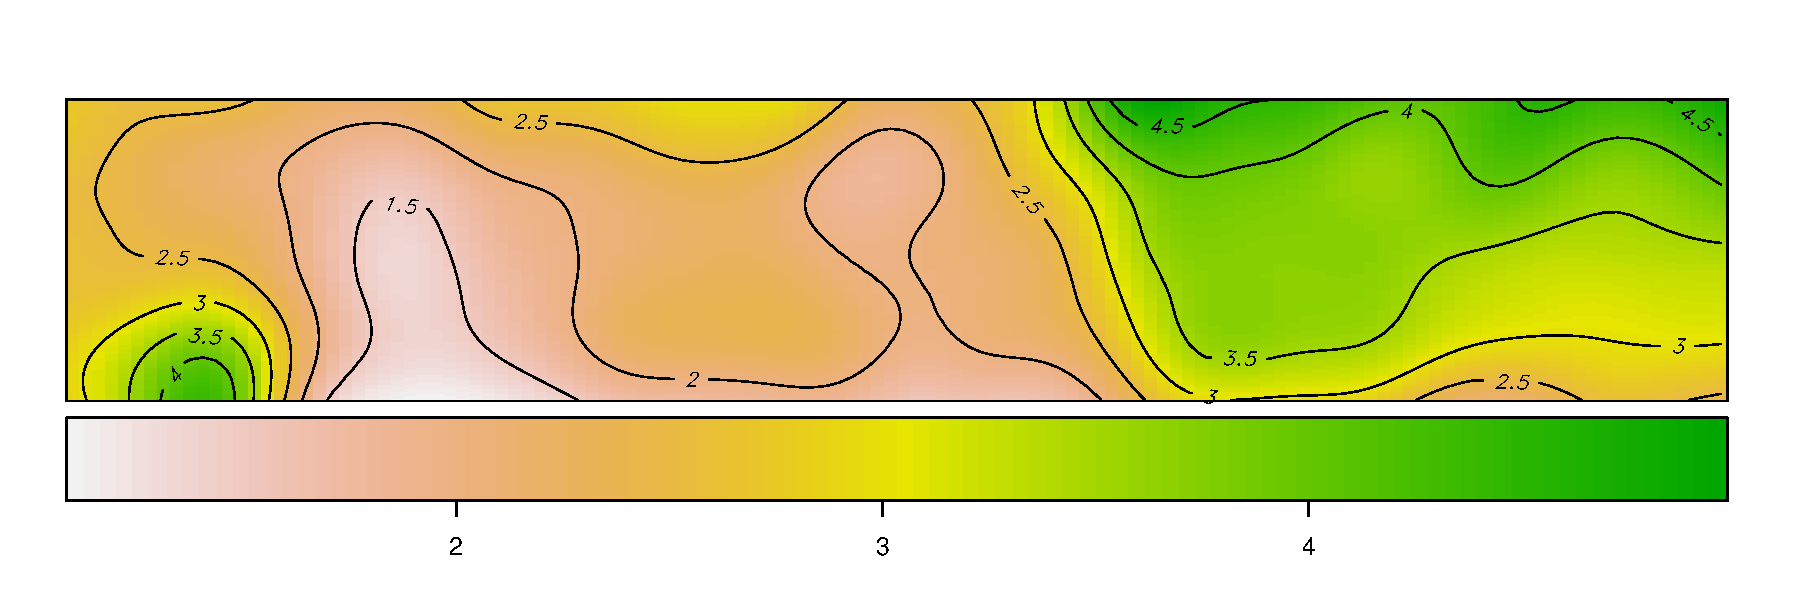
\includegraphics[width=\textwidth]{Images/ST_DiffYield}
% 		\caption{Yield difference of current yield and estimated values with optimal nitrogen.}\label{fig:stdiff}
% 	\end{figure}

	After the optimal nitrogen applied on the field, the estimated product is improved comparing to the yield with current strategy. Figure \ref{fig:stdiff} illustrates the different yield of the two management strategies. The difference is positive and indicates improvement on yield product. 	
	
	\begin{figure}[!htp]
		\centering	
		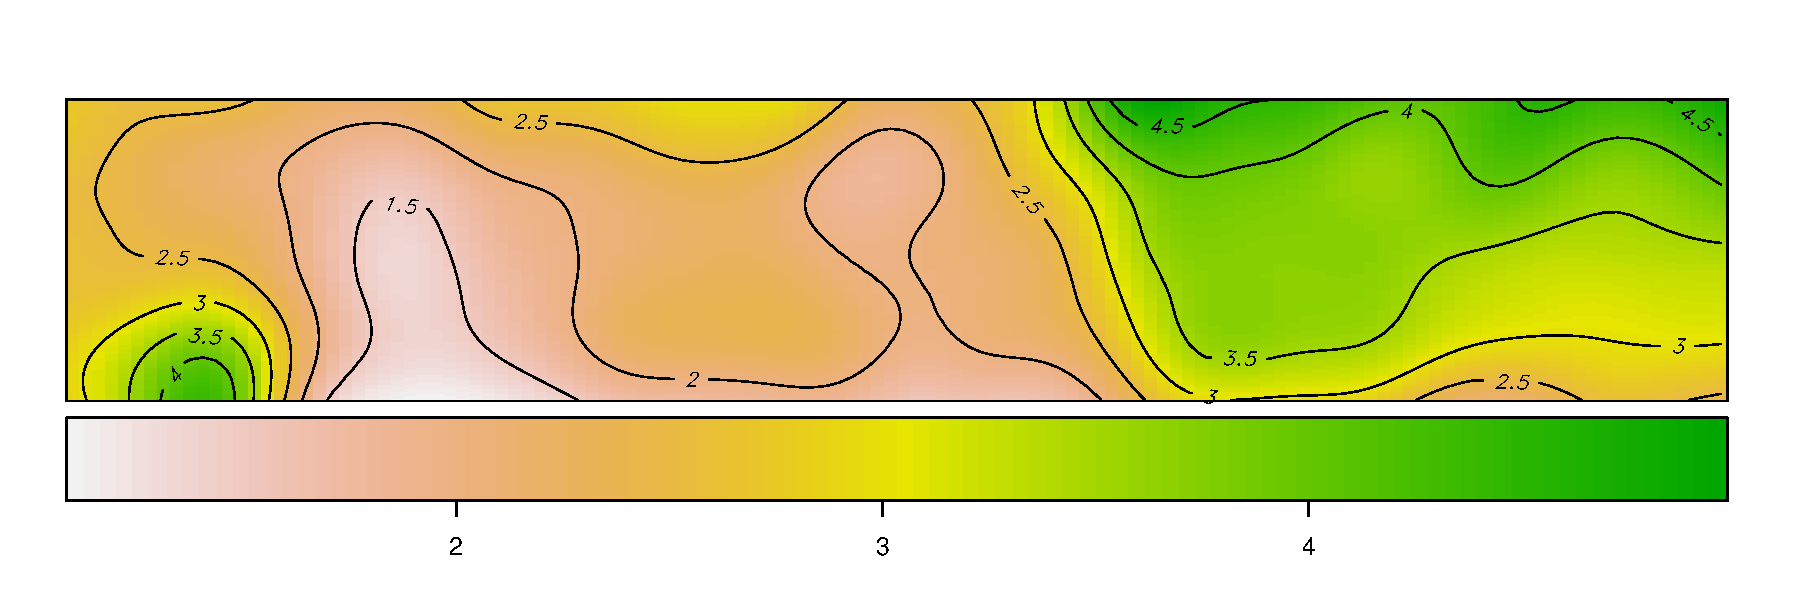
\includegraphics[width=\textwidth]{Images/ST_DiffYield}
		\caption{Yield difference of estimated values with optimal nitrogen and with current nitrogen rate.}\label{fig:stdiff}
	\end{figure}
	
	
	\subsection{Comparing to the GWR approach}\label{sec:comparegwr}
	
	\textcite{Rakshit2020Novel} suggested using geographic weighted regression (GWR) techniques to address the same objective and illustrated the use of a geographic weighted local regression to estimate the optimal nitrogen rate for each plot and to predict the yield for the Las Rosas data set. The Bayesian approach discussed here uses the Bayes theorem, NUTS sampler and Bayesian inference to explore the posterior distribution and the parameters' estimates for each plot. 
	
	The two different approaches aim at the same objective, to providing reliable yield estimates and easy interpretation through visual contour plots, assisting plant growers. Both approaches have their advantages. 
	
	For GWR, the reliability of the results relies on the bandwidth of the moving window. The optimal bandwidth is selected by cross validation. All data points within the window are used for inferring the information of the plot of interest. Other data points, which are out of the window, contribute nothing to the targeted plot. Due to this feature, the data on the boundary of the field are trimmed off, which means the yield and treatment on the boundary are not estimated. GWR has ``higher resolution'' such that the optimal treatments at pairwise plots are distinguishable, even though the adjusted-$p$ values are large. On contrary, the proposed model with a Bayesian approach uses all data with the spatial variance matrix on the entire field to estimate the query plot. The nearer plots contribute more and further plots contribute less to the inference. So it has ``lower resolution'', as it can be seen from Figure \ref{fig:optN} the difference of optimal nitrogen rates in the West and East areas are not significant. Additionally, the reliability of the Bayesian approach is affected by the priors and the model itself, whereas the influence of the prior \textcolor{red}{reduces if the amount of data increases}. Moreover, GWR is an ad hoc approach for addressing a particular question. The Bayesian approach has more flexibility to be extended and to be broadly applied to other questions. 
	
	
	A comparison of these two approaches is summarised in Table \ref{tb:compareGWR}. 
	\begin{table}[!htp]
		\centering
		\begin{tabular}{*{3}{l}} \toprule
			& GWR & Bayesian \\ \midrule
			Inference	& with neighbouring data & with all data \\ 	 
			Initialisation	& bandwidth selection &  prior specification \\ 	
			Objective	& local log-likelihood & global log-likelihood \\ 
			Distinguishability & high & low \\ \midrule
			Evaluation	&  $t$ scores and $p$-values & credible intervals \\
			&  & PP check and LOO PIT \\
			&  & Pareto $k$ diagnosis \\
			&  & Bayesian $R^2$ \\ 
			\bottomrule
		\end{tabular}
		\caption{Comparison of GWR and Bayesian approach.}\label{tb:compareGWR}
	\end{table}
	
	
	\section{Discussion}
	
	In this paper, we demonstrates a Bayesian hierarchical model for the analysis of spatially varying treatment effects in on-farm experiments. We explain the mechanism of a Bayesian approach and the NUTS sampler, which has been proved the ability in sampling highly correlated high-dimensional distributions. NUTS exhibits excellent sampling qualities in terms of generating large effective sample sizes, producing low autocorrelation and obtaining low skewness of marginal posterior distributions \parencite{Nishio2019Performance}. Moreover, NUTS does not require conjugate priors, exhibits faster convergence for multi-parameters and has considerable flexibility for fitting user-specified models by researchers using the \R-package \rstan. However, if the data set is large, computing the inverse of the covariance matrix, which is three times the size of the data, is extremely time consuming by conventional algorithm. Therefore, we implement a faster algorithm for calculating the autocorrelation matrix and develop a faster algorithm for computing the Kronecker product of three matrices. The theory of the algorithms, which can be implemented in \rstan, is presented in the Appendix. 
	
	
	The \Matern class covariance 
	\begin{equation}\label{eq:matcov}
		V_s(d) = \sigma^2 \frac{2^{1-\nu}}{\Gamma(\nu)} \left( \sqrt{2\nu} \frac{d}{r}\right)^\nu K_\nu\left( \sqrt{2\nu} \frac{d}{r}\right),
	\end{equation}
	which is used in spatial analysis \parencite{Cressie1999Classes} and in capturing spatial variation in OFE \parencite{Selle2019Flexible}, can be incorporated in the model as well. %Here, $d$ is the space lag or distance, $r$ is a non-negative scaling parameter, $\nu> 0$ is a smoothness parameter determining the mean-square differentiability of the field, $\sigma_d^2$ is the variance of the process, $\Gamma$ is the Gamma function and $K_\nu$ is the modified Bessel function of the second kind. If $\nu = r + \frac{1}{2}$, then the \Matern covariance can be expressed as a product of an exponential and a polynomial of order $r$. 
	However, the difficulty in implementing the \Matern covariance is the huge amount of time in calculating the inverse of the covariance matrix for thousands of times when the data size is large. As a compromise, we have to either wait for a few days to obtain converged MCMC chains or reduce the effective sample size and terminate the sampling process earlier, which takes the risk of achieving non-converged chains and leaving parts of the space unexplored. In fact, the difference of $\AR\otimes\AR$ and \Matern covariance matrices is not significant, shown in \parencite{Selle2019Flexible}. Practically, $\AR\otimes\AR$ covariance is a satisfying choice for both efficiency and accuracy. 
	
	
	
	The model checking and diagnostic process for post-sampling were presented as well. The Gaussian assumption of the model for the Las Rosas data is misspecified even though the Bayesian $R^2$ value is relatively high. Alternatively, with the help of the diagnostic tools, we discover that Student-$t$ distribution provides a more robust inference. The Bayesian $R^2$ is misleading in some situations, and should not be interpreted solely. 
	
	
	
	Finally, in Section \ref{sec:comparegwr}, we compare with GWR approach. The proposed Bayesian approach does not require bandwidth selection, but requires pre-specified priors. The results from the Bayesian approach are similar to the ones from GWR and the approach is able to capture more detailed information for the field. Additionally, the GWR trims off the edges of the data on the field due to the fact that it requires the neighbouring data to interpolate the query grid with local log-likelihood. On the contrary, the Bayesian approach uses all data to obtain a smooth map. 
	
	
	
	\section{Conclusion}
	
	The novelty of our work can be summarised as follows:
	\begin{itemize}
		\item Adapts a Bayesian hierarchical model to large on-farm strip trials.
		\item The model consists of a global term and a spatially correlated random term.
		\item The Bayesian inference of all parameters is estimated by faster Kronecker product computing algorithms in \rstan.
		\item Advanced diagnostic tools spot out potential model misspecification. 
		\item Compared with GWR, each approach shows its advantage. 
	\end{itemize}
	
	Both the proposed Bayesian and GWR approaches can only fit regular-shaped data set. If zig-zag pattern appear on the edge of the field, or the data are collected in irregular-space, a further investigation should be carried out. 
	
	
	
	\section*{Authors’ contribution}
	
	Zhanglong Cao: Conceptualization, Methodology, Writing - Original Draft, Writing - Review \& Editing, Visualization; Katia Stefanova: Writing - Original Draft, Writing - Review \& Editing; Mark Gibberd: Writing - Review \& Editing, Project administration; Suman Rakshit: Conceptualization, Methodology, Writing - Review \& Editing, Supervision. 
	
	
	\section*{Acknowledgement}
	
	The authors gratefully acknowledge the support from the Grains Research and Development Corporation of Australia (GRDC). 
	
	
	
	\appendix
	\addcontentsline{toc}{section}{Appendices}	
	\section*{Appendix}
	
	\section{Prior predictive checking}\label{App:Prior}
	
	\begin{figure}[!htp]
		\centering
		\begin{subfigure}[t]{0.45\textwidth}
			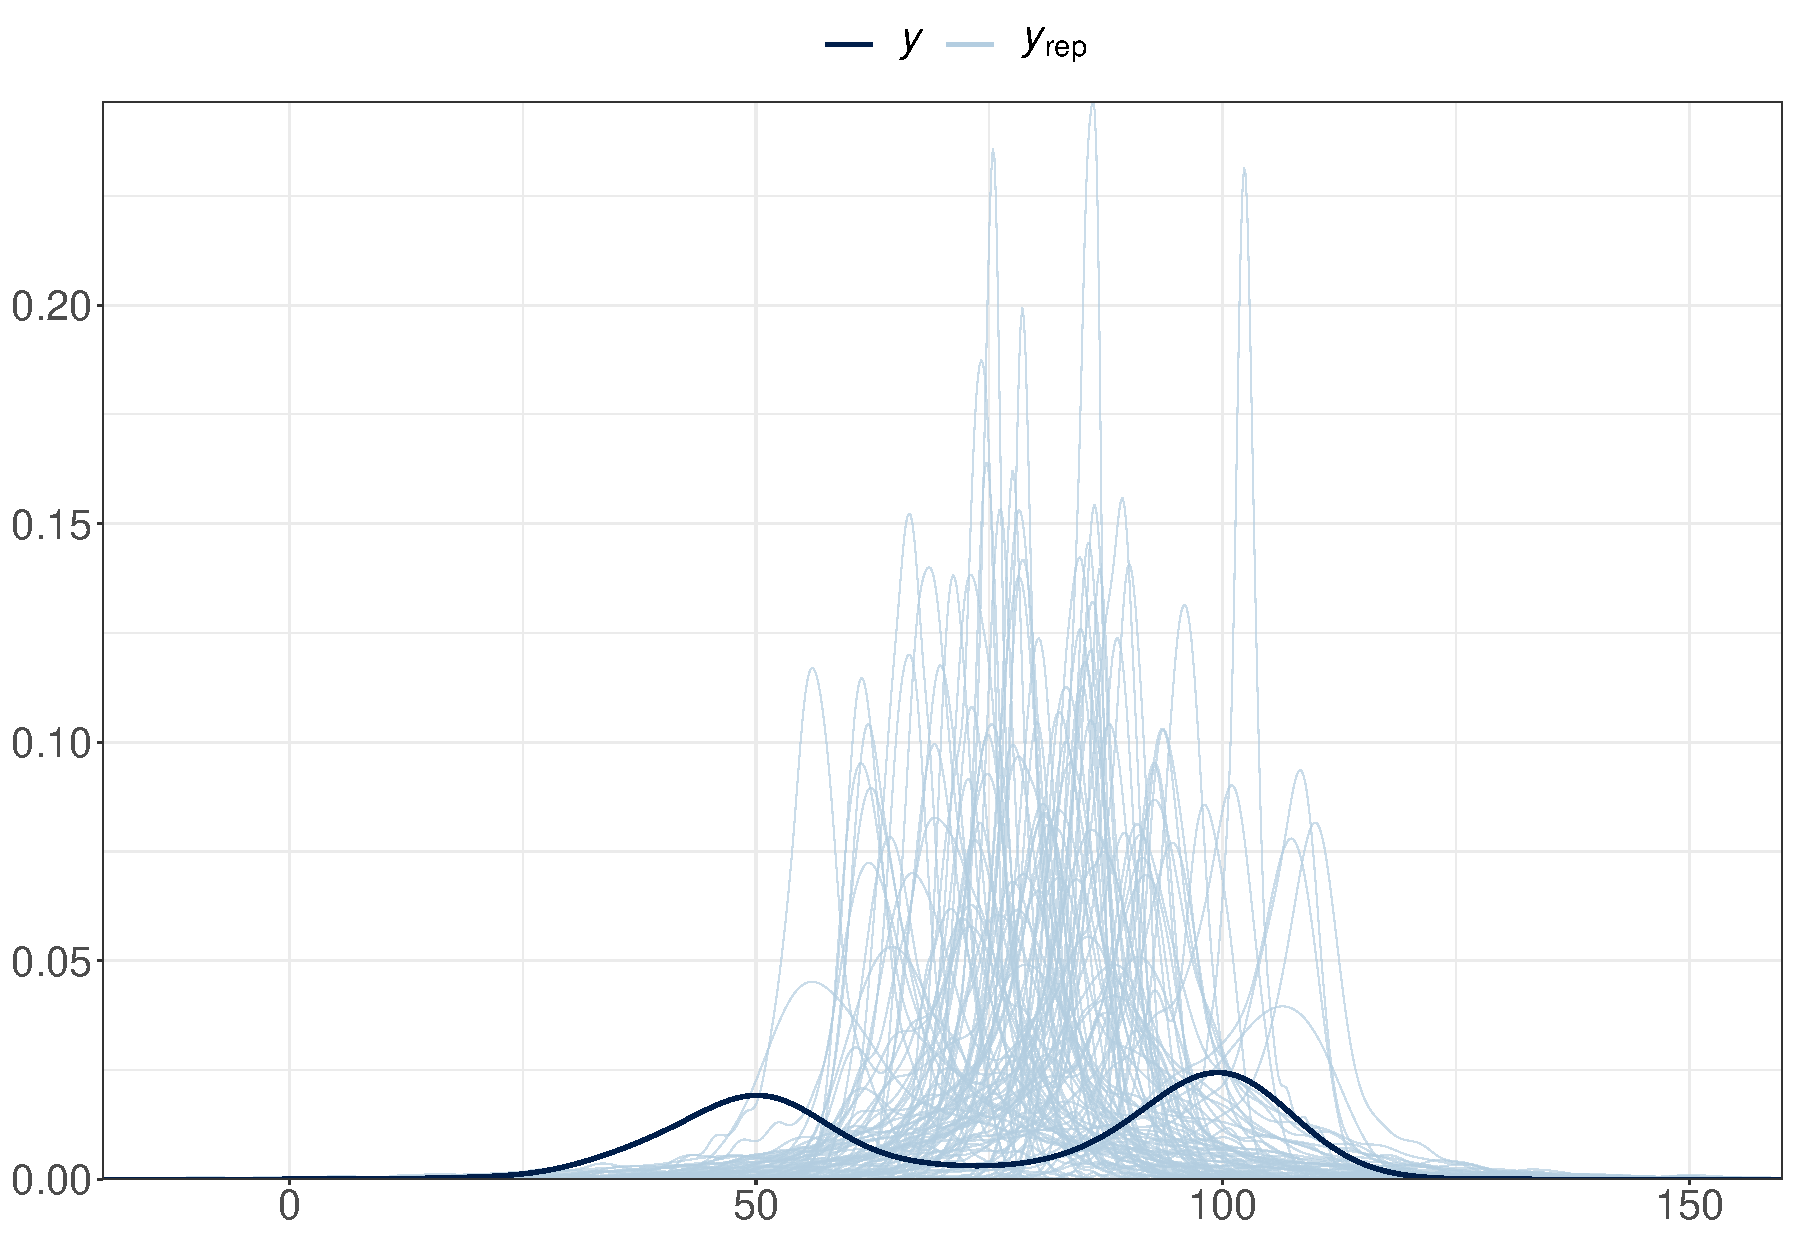
\includegraphics[width=\linewidth]{Images/prior_GSRNS}
			\caption{Model 1: Gaussian distribution without spatial correlation.}
		\end{subfigure}
		\begin{subfigure}[t]{0.45\textwidth}
			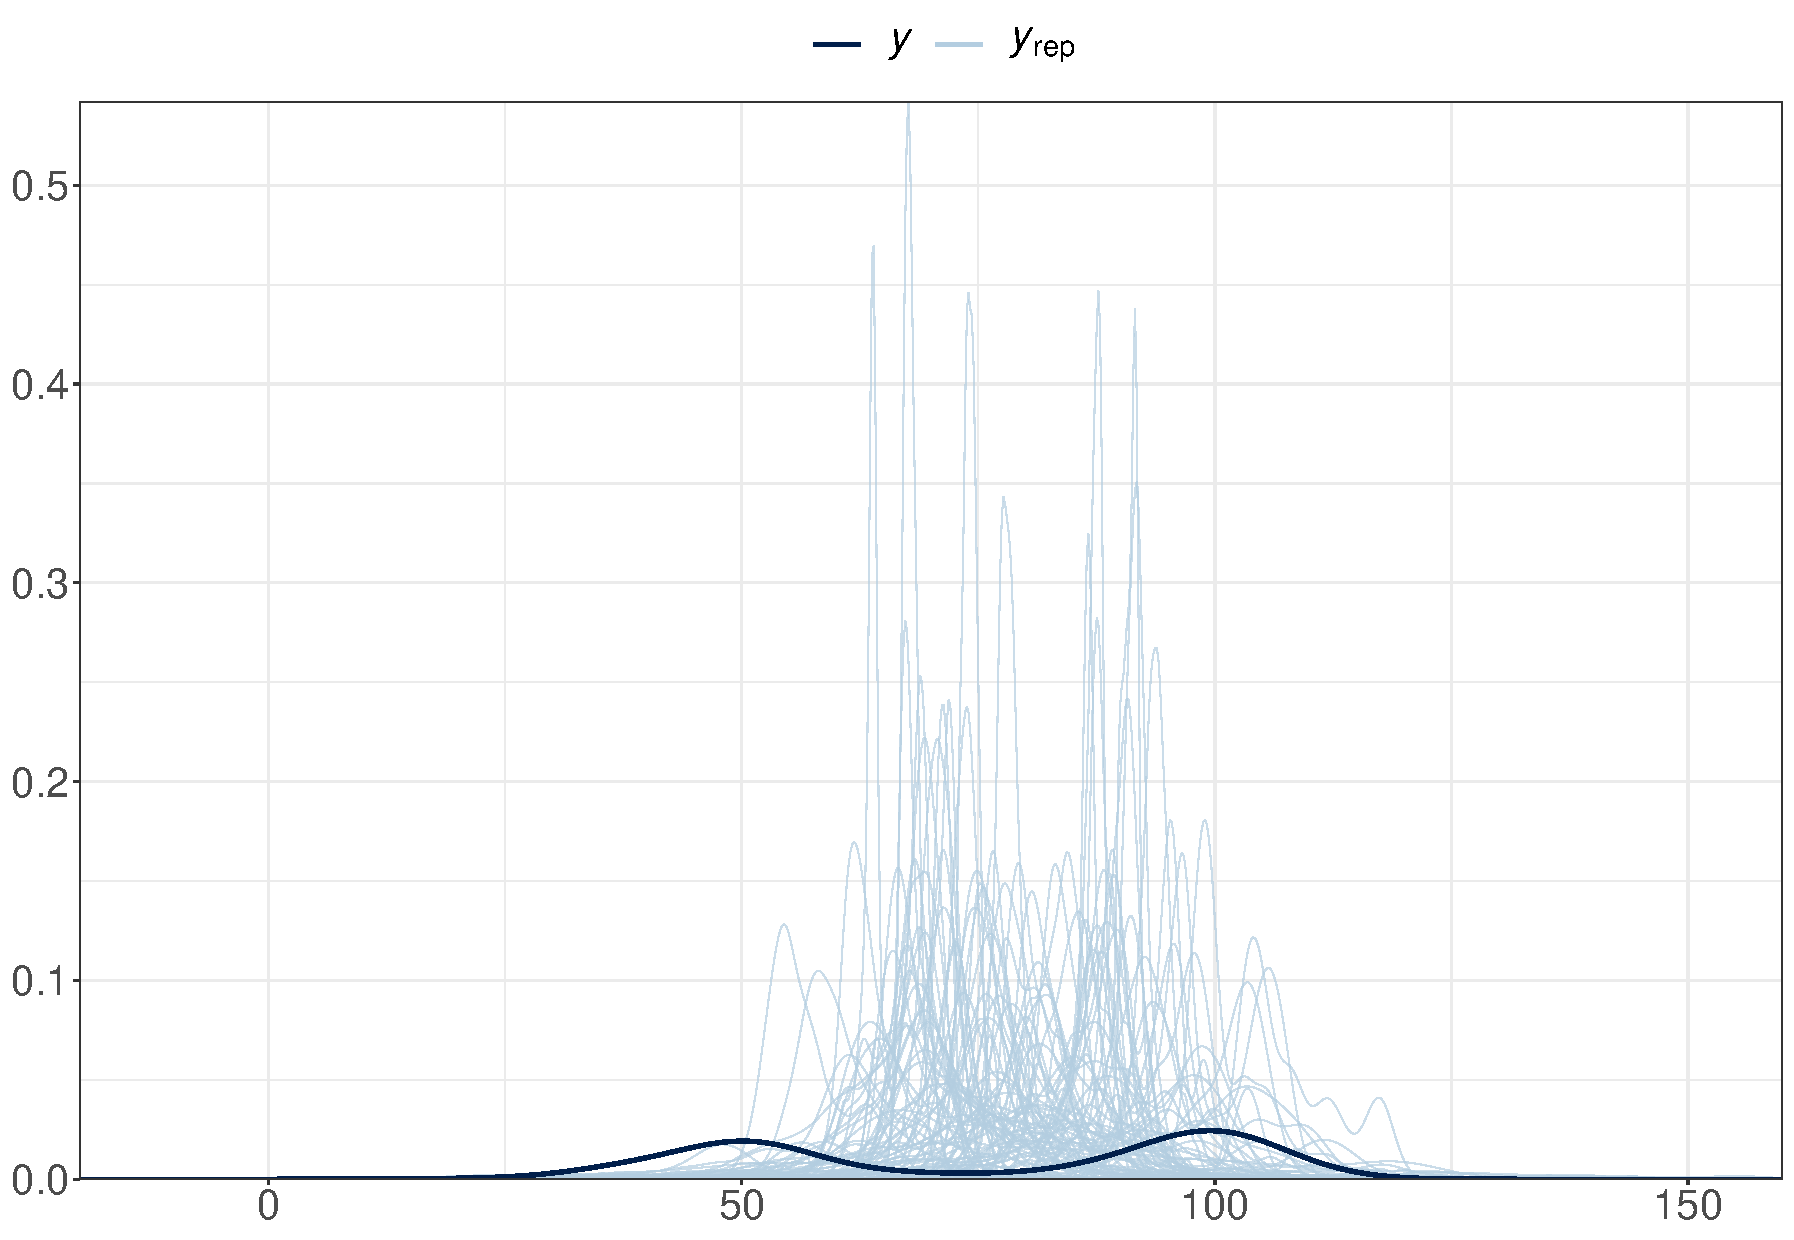
\includegraphics[width=\linewidth]{Images/prior_GSRand}
			\caption{Model 2: Gaussian distribution with spatial correlation.}
		\end{subfigure}
		\begin{subfigure}[t]{0.45\textwidth}
			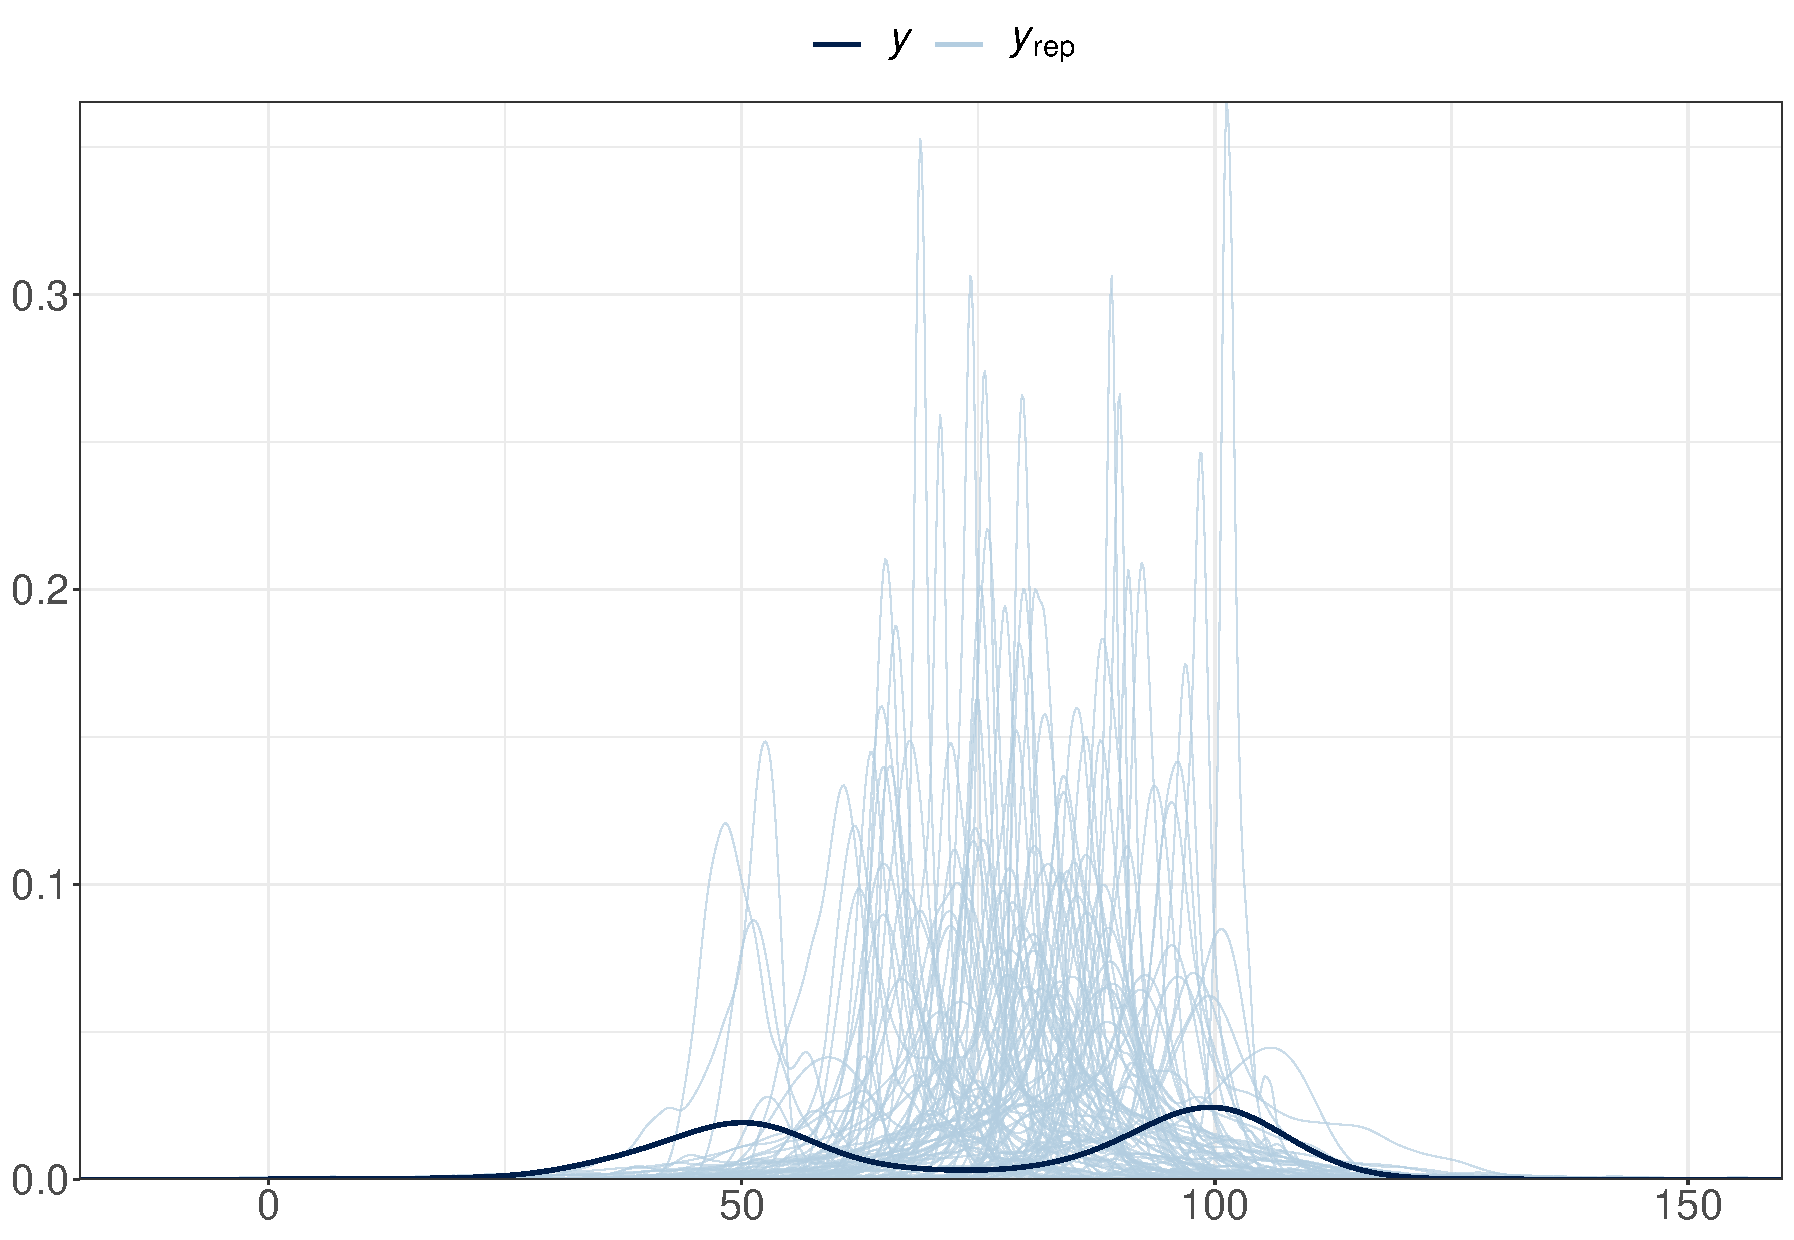
\includegraphics[width=\linewidth]{Images/prior_STRNS}
			\caption{Model 3: Student distribution without spatial correlation.}
		\end{subfigure}
		\begin{subfigure}[t]{0.45\textwidth}		
			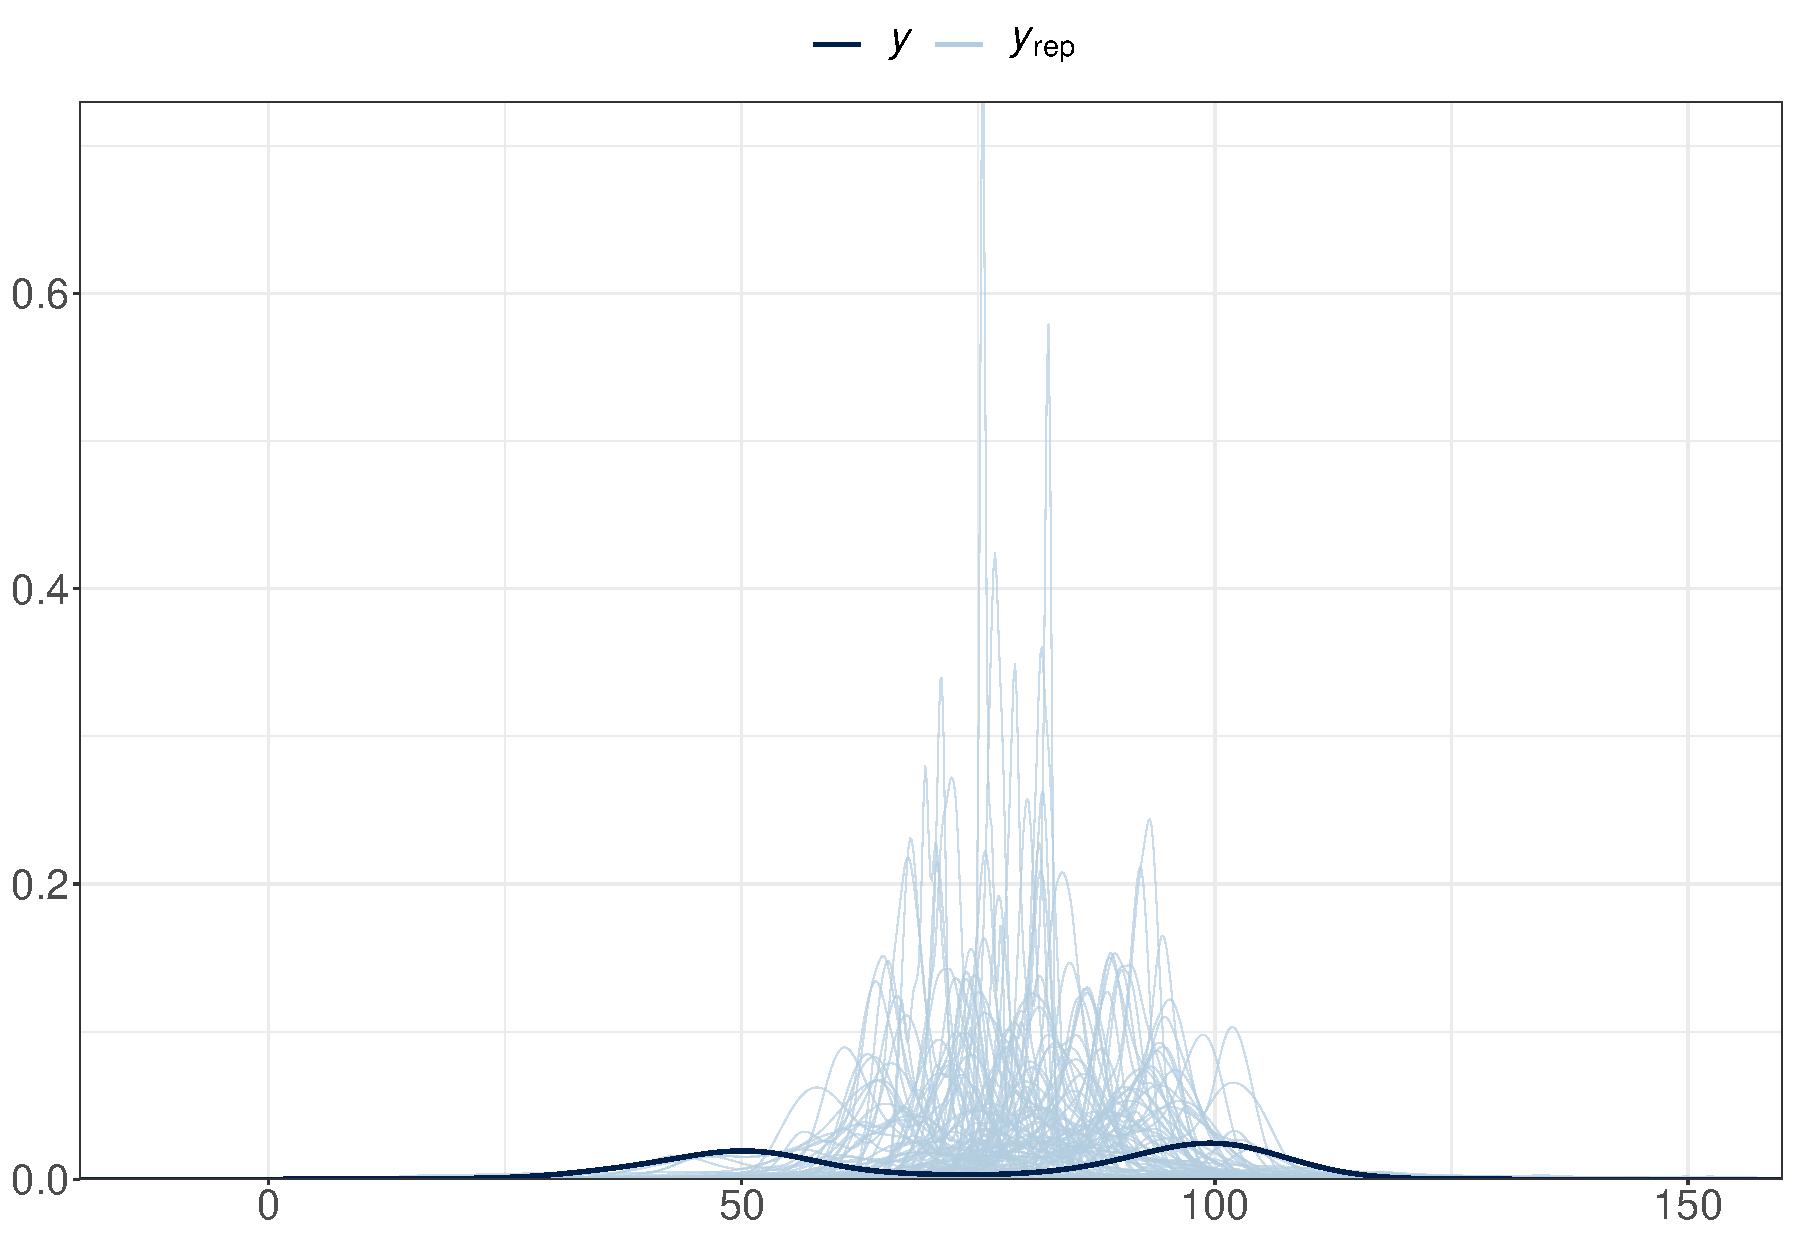
\includegraphics[width=\linewidth]{Images/prior_STRand}
			\caption{Model 4: Student distribution with spatial correlation.}
		\end{subfigure}
		\caption{Weakly informative priors checking for four models. }\label{fig:priorcheck4models}
	\end{figure}
	
	
	\section{Faster Cholesky factor for $\AR(\rho)$}\label{sec:fastar1}
	
	The $\AR(\rho)$ correlation matrix with correlation coefficient $\rho$ is defined as $\rho_{ij} = \rho^{|i-j|}$. A simple form of Cholesky factor for the $\AR(\rho)$ structure, given by \textcite{Madar2015Direct}, was used 
	\begin{equation}
		l_{ij} = \begin{cases}
			\rho^{j-1} & j\geq i =1 \\
			\rho^{j-i} \sqrt{1-\rho^2} & j\geq i \geq2
		\end{cases},
	\end{equation}
	which significantly improved the computational efficiency in \rstan. 
	
	\section{Fast Kronecker product}\label{sec:kronec}
	
% 	Assume $A=L_A L_A^\top$ and $B=L_B L_B^\top$ are respectively $N\times N$ and $M\times M$ matrices with \textcolor{red}{lower triangular factors of} Cholesky decomposition $L_A$ and $L_B$. One good property of the Kronecker product is that
% 	\begin{equation}
% 		C=A\otimes B = (L_A L_A^\top)\otimes (L_B L_B^\top) = (L_A\otimes L_B)(L_A \otimes L_B)^\top,
% 	\end{equation}
% 	where the new matrix $C$ is $NM\times NM$, and the elements of the new matrix are  $c_{p,q}=a_{i,j}b_{k,l}$, where $p=M(i-1)+k$ and $q=M(j-1)+l$. Similarly, the Kronecker product of three matrices, with a $K\times K$ matrix $C$, is
% 	\begin{equation}
% 		D=A\otimes B\otimes C = (L_A L_A^\top)\otimes (L_B L_B^\top)\otimes (L_C L_C^\top) = (L_A\otimes L_B\otimes L_C) (L_A\otimes  L_B\otimes L_C)^\top,
% 	\end{equation}
% 	and the new elements are $d_{p,q}=a_{i,j}b_{k,l}c_{m,n}$, where $p=K(M(i-1)+k-1)+m$ and $q=K(M(j-1)+l-1)+n$. 
	
	
	Let $A=[a_1,a_2,\ldots,a_n]\in \mathbb{R}^{m\times n}$, where $a_j\in\mathbb{R}^m, j=1,2,\ldots,n$. Then the vector $\mbox{vec}(A)$ is defined as 
	\begin{equation}
		\mbox{vec}(A) = [a_1,a_2,\ldots,a_n]^\top \in \mathbb{R}^{mn}, 
	\end{equation}
	which vec-permutes the given matrix. With the vector-valued operator, we have the ``Vec Trick'' theorem: 	
	\begin{lemma} (Roth's Column Lemma: ``Vec Trick'' \parencite{Roth1934Direct, Airola2018Fast} ): Let $A \in \mathbb{R}^{m\times n}$, $B \in \mathbb{R}^{n\times p}$, and $C \in \mathbb{R}^{p\times q}$ be matrices. Then
			\begin{equation}
			 \mbox{vec}(ABC) =	(C^\top \otimes A)\mbox{vec}(B). 
			\end{equation}
	\end{lemma}
	
	The above property and theorem are implemented in \rstan\ and considerably saved computation time. For other properties of the Kronecker product see \textcite{Zhang2013Kronecker}.
	
	
	\renewcommand\bibname{References}% change bibliography title to references
	%\addcontentsline{toc}{chapter}{Bibliography}
	\addtocontents{toc}{Bibliography}
	\printbibliography
\end{document}
